% USC Dissertation/Thesis LaTeX Template
% Edited by Ruda Zhang, 2020-10-08.
% -----------------------------------------------------------------------------
%	PACKAGES AND DOCUMENT CONFIGURATION
%-----------------------------------------------------------------------------

% Use `report` class with `USCthesis` package (style file) by Brian P. Gerkey
% Font size should be 11 or 12 points for regular paragraph text.
\documentclass[letterpaper,12pt]{report}
% [options] can be any of these default/alternative flag:
%   dissertation/thesis, final/proposal, copyright/nocopyright,
%   fussy/sloppy, flushbottom/raggedbottom, clref/opref.
\usepackage[dissertation, final, opref, raggedbottom]{USCthesis}

% Packages required by `USCthesis.sty`.
\usepackage{hyperref}
\usepackage{setspace}
\usepackage{tabularx}
\newenvironment{myepigraph}
  {\par\hfill\itshape
   \begin{tabular}{@{}r@{\hspace{2em}}}} % 2em from the right margin
  {\end{tabular}\par\medskip}
% Line spacing and margins in compliance with USC graduate school guidelines.
\usepackage[margin=1in,footskip=.5in]{geometry}
\doublespacing

% Optional packages: mathematical fonts and symbols
% You may comment this section out if you don't need them.
\usepackage{mathptmx} % set font to Times Roman
\usepackage[OT1]{fontenc} % font encoding for xelatex
\usepackage{mathtools}
\usepackage{amsmath}
\usepackage{amssymb}
% Optional packages: graphics
\usepackage{graphicx}
% You can use the "demo" option while editing to avoid compiling figures.
% \usepackage[demo]{graphicx}
% You can add absolute paths as well.
\graphicspath{{./}{../}{figures/}{../figures/}{main/rvagene/figures}}
% Optional packages: bibliography with BibLaTeX.
% Comment this section out if you prefer BibTeX.
%\usepackage[
%    style=nature,
%    sorting=none,
%    isbn=false,
%    url=false,
%    doi=true,
%    eprint=false,
%    date=year,
%    maxnames=6,
%    minnames=6
%]{biblatex}
%\AtEveryBibitem{\clearfield{eventtitle}} 
%\AtEveryCitekey{\clearfield{eventtitle}}
%\AtEveryBibitem{\clearfield{pagetotal}} 
%\AtEveryCitekey{\clearfield{pagetotal}}
%\addbibresource{references.bib}

% Filler text for formatting. Comment these lines out for real writing.
\usepackage[english]{babel}
\usepackage{blindtext}
%%%%%%%%%%%%%%% My Additions ############

%\usepackage[top=0.85in,left=2.75in,footskip=0.75in,marginparwidth=2in]{geometry}
\usepackage{pmi} %pmi piyush rai style
%\usepackage{ml}
% use Unicode characters - try changing the option if you run into troubles with special characters (e.g. umlauts)
\usepackage[utf8]{inputenc}
\usepackage[lining,semibold]{libertine} % a bit lighter than Times--no osf in math
\usepackage[varqu,varl]{inconsolata}% a typewriter font must be defined
% clean citations
%\usepackage{cite}
% hyperref makes references clicky. use \url{www.example.com} or \href{www.example.com}{description} to add a clicky url
\usepackage{nameref,hyperref}
\hypersetup{
  colorlinks   = true, %Colours links instead of ugly boxes
  urlcolor     = blue, %Colour for external hyperlinks
  linkcolor    = blue, %Colour of internal links
  citecolor    = blue  %Colour of citations
}
% line numbers
\usepackage[right]{lineno}
\newcommand\numberthis{\addtocounter{equation}{1}\tag{\theequation}}

% improves typesetting in LaTeX
\usepackage{microtype}
\DisableLigatures[f]{encoding = *, family = *  }
\usepackage{wrapfig}

% text layout - change as needed
%-------------------------------------------------
% \raggedright
% \setlength{\parindent}{0.5cm}
% \textwidth 5.25in
% \textheight 8.75in
%--------------------------------------------------
% Remove % for double line spacing
%\usepackage{setspace}
%\doublespacing

% use adjustwidth environment to exceed text width (see examples in text)
\usepackage{changepage}

% adjust caption style
\usepackage[aboveskip=1pt,labelfont=bf,labelsep=period,singlelinecheck=off]{caption}


\makeatletter
\renewcommand{\@biblabel}[1]{\quad#1.}
\makeatother
%\usepackage[numbers]{natbib}
\usepackage[backend=biber, style=numeric, sortcites, maxnames=10, natbib=true]{biblatex}
\usepackage{csquotes}% Recommended
\usepackage{pmi}
%\bibliography{library}
\addbibresource{library.bib}

\newcommand{\tcr} { \textcolor{red} }

\newcommand{\scrna}{scRNA-seq }

\makeatletter
\renewenvironment{abstract}{%
  \if@twocolumn
    \section*{\abstractname}%
  \else
    \small
    \begin{center}%
      {\bfseries \abstractname\vspace{-.5em}\vspace{\z@}}%
    \end{center}%
    \quotation
  \fi}
  {\if@twocolumn\else\endquotation\fi}
\makeatother


\begin{document}

%-----------------------------------------------------------------------------
%	TITLE PAGE
%-----------------------------------------------------------------------------

% Volume name could be added as option, e.g. `[Volume I]`.
\title{\textbf{\Large{Deciphering Protein-Nucleic Acid Interactions with Artificial Intelligence}}}

\author{Raktim Mitra}

% Committee list is only shown in `proposal` layout.
\committee{A.~Remo Rohs & (Chair)\\*
           B.~Adam MacLean\\*
           C.~Fengzhu Sun\\*
           D.~Helen Berman \\*
           E.~Aiichiro Nakano & (Outside Member)}

% Submission information is only shown in `final` layout.
\majorfield{Computational Biology and Bioinformatics}
\submitdate{December 2024}  % Must be one of the three dates allowed in the guideline

% Make sure everything, specially your title page, exactly follows the guideline:
% https://graduateschool.usc.edu/wp-content/themes/fictional-university-theme/assets/doc/Manuscript_Formatting_and_Documentation_Styles.pdf

%-----------------------------------------------------------------------------
%	PREFACE
%-----------------------------------------------------------------------------

% The preface environment prints the title page.
\begin{preface}
  
  \prefacesection[Epigraph]{Epigraph}
  \topskip0pt
\vspace*{\fill}
\vspace*{-2in}
\begin{myepigraph}
\large
``Karmanye v$\bar{\text a}$dhik$\bar{\text a}$raste M$\bar{\text a}$ Phaleshu Kad$\bar{\text a}$chana,\\ 
\large 
M$\bar{\text a}$ Karmaphalaheturbh$\bar{\text u}$rm$\bar{\text a}$ Te Sangostvakarmani."\\
\large $-$Srimadbhagabatgita,  S$\bar{\text a}$nkhya Yoga (Dwitiya Adhyaya), Sloka 47
\end{myepigraph}
%\epigraph{Karmanye vadhikaraste Ma Phaleshu Kadachana,\\ Ma Karmaphalaheturbhurma Te Sangostvakarmani}{Srimadbhagabatgita,  Sānkhya Yoga (47) }
\vspace*{\fill}

  % Dedication Page, which is truly unnecessary.
  \prefacesection[Dedication]{Dedication}
  \topskip0pt
\vspace*{\fill}
\vspace*{-2in}
\begin{quote}
    \center
    I dedicate this dissertation to $Hiren$ and $Mahua\;Mitra$, \\
    for their never ending love and support.
\end{quote}
\vspace*{\fill}


  % Acknowledgement Page, which is also unnecessary for proposals.
  \prefacesection{Acknowledgements}
  %% CHANGE NAMES AND WRITING

I offer my utmost thanks to my advisor Prof. Remo Rohs, whose encouragement, patience, intelligent decisions and immense knowledge supported me throughout my Ph.D., made it a wonderful experience, and helped me overcome many difficulties.

I am also extremely thankful to my dissertation committee members Prof. Helen M. Berman, Prof. Fengzhu Sun, Prof. Adam L. MacLean and Prof. Aiichiro Nakano, and qualifying exam committee member Prof. Xiaojiang Chen. Their insightful comments enriched and widened my research from various perspectives. 

I joined the QCB department at USC as a PhD student in August 2019. The rigorous curriculum of the CBB PhD program helped me shape my scientific vision and research skills. Soon, the COVID-19 pandemic changed everything about our life and uncertainty covered the world. Thankfully, due to wise and loving care of the department, my advisor Prof. Remo Rohs and other members of the QCB department, I was able to continue my work through the difficult times. Prof. Adam MacLean worked hard to help me finish the RVAgene project and get it published \citep{Mitra2021}. The pandemic affected scientific travel opportunities severely, during those initial years of my PhD. However, later on I was fortunate to be able to travel to numerous high quality conferences and present my work there. I am thankful to my advisor Prof. Remo Rohs for providing me with these opportunities. In fact, meeting Nobel laureate Prof. Ada Yonath (for solving the structure of ribosome \citep{schluenzen2000structure, harms2001high}) has been one of the most memorable experiences of my life. I am also thankful to prof. Yonath for supporting us on the RNAscape project. Traveling to conferences and presenting my work through posters and oral presentation opened up a lot of career and collaboration opportunities for me. My scientific thinking has been shaped by these experiences, coupled with professional growth. I am grateful to the Rohs Lab members for accompanying and participating alongside me in these events and for always being supportive and encouraging.

I also present my gratitude to my collaborator Dr. Cameron Glasscock from the David Baker lab at University of Washington, and to Prof. Ada Yonath and her lab members, for being supportive to my research. 

I am thankful to the Andrew Viterbi Fellowship in Computational Biology and Bioinformatics for supporting me over three years of my PhD.

My sincere thanks goes to the QCB department for allowing me to participate in various departmental activities which helped shape me as a person. It has been a pleasure to work with and receive all forms of support from Rokas, Tanya, Katie and Christian.

I thank my fellow labmates Yibei, Tsu-pei, Jinsen, Ari, Jesse, Yingfei, George, previous lab members Brendon and Jared. This dissertation would not have been possible without their stimulating discussions and contributions, both in science and in life. Specially, without Jared's mentorship during the earlier years of my PhD, my dissertation would not be able to achieve its current form. I also thank my graduate mentees Zijin, Wei Yu, Chan, Lexi (and others), and my undergraduate mentees Andrew, Hirad, Avinash and Irika. It has been a pleasure to work with all of you and to see your scientific growth. 
Special thanks go to my friends Bryan, Meilu, Sophia, Vivian, Fred, Eric, Priyanka, Chloe, Nic and Anik, for supporting me along the way. You have made my life in Los Angeles a pristine remembrance. I also offer my gratitude to Prof. Lina Bahn, Christine Lee, Yue Qian, and Haesol Lee, for helping me pursue my interest in violin and music, which helped me conquer many challenging times.

Last but not the least, I am forever indebted to my parents without whose decades long hard work and dedication I would not even be here. On the same thread, I am grateful for the support of my extended family members and childhood friends and teachers, who provided me with unfailing support and continuous encouragement throughout the journey.
{
  \hypersetup{linkcolor=black}
  \tableofcontents
  \listoffigures*
  \listoftables   % Comment this out if you don't have tables

}

  % Abstract Page
  \prefacesection{Abstract}
  This dissertation contains an account of my research work during my PhD at University of Southern California.
My primary focus has been deciphering protein-DNA interaction with data driven deep learning methods. I present, in chapter 1,
my work on the segmentation of protein surfaces into nucleic acid binding and non-binding regions. This chapter describes a graph neural network layer, which enables smooth prediction of binding site labels on the protein surface. We start from a model of nucleic acid binding site
prediction (PNAbind) developed in the Rohs lab and improve upon it by designing a neural network layer using mean field
VI over a continuous Conditional Random Field model, which makes the predicted binding sites smoother while improving upon prediction metrics. We also design a smoothness metric
addressing the label imbalance problem associated with the task.
In Chapter 2, I describe DeepPBS (Deep predictor of binding specificity), the first of its kind geometric deep learning method developed to predict DNA binding specificity of proteins based on a given protein-DNA complex. DeepPBS acts as a bridge between structure determining (which shows mechanism but not sequence diversity) and specificity determining experiments (which reflects sequences diversity but not mechanism). DeepPBS is applicable on experimentally determined, simulated, predicted or designed complexes, resulting in a broad impact in the domain.
In chapter 3, we design and showcase the RNAscape algorithm and webserver, a geometric mapping method of RNA 3D structures to 2D, which attempts to preserve the three dimensional topology (unlike common secondary structure based visualization methods). RNAscape significantly improves over existing competitors in terms of the mapping quality, visualization and customisability.
Chapter 4 describes an updated DNAproDB database, which was originally implemented by Jared Sagendorf. Through this update we
introduce both technical advances and an expansion of features included in the analysis.
DNAproDB is now automatically updated weekly with newly released structures and thereby will
remain up to date as new DNA–protein structures are solved. We also include much larger
complexes, expand external annotations and upload/download formats, and improve the user
experience through a re-organization of the web interface and more visualization options and
controls. We added the annotation of water-mediated hydrogen bonds as a new feature.
At the same time we recognized lack of a comprehensive analysis and exploration tool for RNA/protein-RNA structures. Being inspired from RNAscape and DNAproDB, we developed RNAproDB, which is described in Chapter 5. RNAproDB is a modern highly interactive structure exploration tool tailored for the complexity and structural variance of RNA structures. This is achieved by intricate interplay of a 3D viewer, interface explorer, sequence viewer, secondary structure selector and tabular data:  making it the most versatile tool for analyzing and exploring protien-NA complexes. With the advent of complex structure prediction methods like AlphaFold3, we expect RNAproDB to serve a crucial role in analyzing predicted structures and advance the understanding of cellular biology.
In chapter 6, I present an autoencoder model applicable on gene expression time-series data, to learn a regularized latent
space representation and a generative process. RVAgene is primarily a visualization tool suitable for biological
knowledge discovery, while also being suitable for de novo data generation, denoising and a more
efficient alternative to hierarchical Gaussian process based methods to cluster such data. We
analyze one synthetic and two real datasets and demonstrate various properties and aspects of the
model and its potential for unsupervised discovery.  In particular, RVAgene identifies new programs of
shared gene regulation of \textit{Lox} family genes in response to kidney injury. We conclude this thesis by discussing current state of the field of structural biology of protein-nucleic acid complexes and discussing future possibilities.

\end{preface}

%-----------------------------------------------------------------------------
%	CONTENT STRUCTURE
%-----------------------------------------------------------------------------

% Better to separate LaTeX structure and content


%%%%%%%%%%%%%%%%%%%%%%%%%%%%%%%%%%%%%%%%%%%%%%%%%% CRF %%%%%%%%%%%%%%%%%%%%%%%%%%%%%%%%%%%%%%%%%%%%%%%%%%%%%%%%%%%%%%%%%%%%%%%%%%%
% More Research Topics
% \include{ResearchTopic2}

\chapter{A probabilistic model for smooth binding site label prediction on protein surfaces}
\label{cha:research_topic_2}

\vspace*{0.35in}

\begin{flushleft}

%{\large Raktim Mitra\textsuperscript{1}, 
%Jared Sagendorf\textsuperscript{1}}\\

%\bigskip
%$^1$Quantitative and Computational Biology, University of Southern California
%\\


\end{flushleft}

\begin{abstract} 
    Predicting DNA/RNA binding sites on a given protein surface is an important computational task since experimentally determining such information is often expensive and time consuming. Such binding site prediction task can be formulated as a node classification task over a 3D mesh representing the protein surface, with features over the vertices and edges of the mesh representing various geometrical and physicochemical features of the protein structure. At our lab we developed a deep learning based method, which independently classifies mesh vertices as binding and non-binding sites. This often results in irregular binding site predictions over the protein surface. However, intuitively, binding site predictions should be contiguous and not patchy i.e. as ``smooth" as possible while being correct. In this chapter, we describe what such kind of ``smoothness" entails and we improve upon the original architecture by designing a network layer based on a  probabilistic Continuous Conditional Random Field (CCRF) model, which increases smoothness of binding site prediction while improving prediction accuracy of the model. This network layer was incorporated into the original model and will be published as the Geobind package (Sagendorf et. al).
\end{abstract}

\section{Introduction} Predicting DNA/RNA binding sites on protein structures is an important
computational task.  There are many existing methods which attempt to solve this problem either on
the sequence level or on 3D structure level based on either sequence features or structural features
of proteins \citep{deng2018pdrlgb, wang2010bindn+, wang2006bindn, li2013predna}
.We  represent protein surfaces as 3D triangulated meshes with 
vertices and edges having features representing different geometrical and physicochemical aspects
of the protein structure. Now, we can learn a model which classifies each vertex of such a mesh to either binding-site or
non-binding sites. With recent advances in 3D deep learning, Graph Convolutional
Networks(GCNs) have come out as a useful approach for learning higher level features over
3D mesh objects. We developed a GCN based deep learning model for the binding site classification
task: Geobind. \hyperref[fig:crf_concept]{Fig. 1.1A} shows a schematic diagram of
the task Geobind achieves.

Standard neural network approach is to predict each binding-site label independently
through it's output layer. However, classification tasks often come with additional non-trivialities which
are not addressable with independence assumption.  For example, image segmentation task involves
classifying every pixel of an image (which can be thought of as a grid of pixels) to some class.
However, independence assumption often gives poor/scattered results. In that case, some form of
conditional label (re)assignment is necessary for each pixel considering its neighbouring pixels. The
most common way to achieve the same in the field of computer vision is via optimizing a conditional
random  field (CRF) model over a set of initially  learned labels. For example,
\hyperref[fig:crf_concept]{Fig. 1.1B} adapted
from \citet{krahenbuhl2012efficient}  shows how an implementation based on CRF can improve image
segmentation results. In our case, we also expect certain properties from a predicted binding site
region on a protein surface. A binding site region on a protein surface is basically a combination
of multiple mesh vertices predicted as binding sites. We generally expect such a region to be
"smooth" i.e. not randomly have misclassified points scattered around. This idea is visually illustrated in
\hyperref[fig:crf_concept]{Fig. 1.1C}. So, we need to do some kind
of conditional (re)assignment of class labels generated by our Geobind network.

In addition to Computer vision, CRF models are also heavily used in Natural Language processing (NLP)
\citep{roark2004discriminative,mccallum2003early,liu2017identification}. However, both in Computer
vision and NLP, the underlying graph structure, over which the CRF is defined, is very sparse and
simple e.g. linear chain or tree for NLP and 2D grid for computer vision. Which makes it easy to
find some form of optimization scheme on the discrete domain of labels. However, this is not the
case for a general underlying graph, where the combinatoriality of the possible label assignments
for all vertices is huge and in the discrete domain of labels there is no gradient information for
efficient optimization.

\citet{krahenbuhl2012efficient} proposes an efficient inference algorithm for fully connected CRFs
based on mean field Variational Inference and high dimensional filtering using permutohedral lattice
approximation. However, the high dimensional filtering step is not compatible with
SIMD\citep{nickolls2008scalable} paradigm of GPU computation. \citep{teichmann2018convolutional}
making it impossible to use on large datasets and non-trivial graphs.
\citet{teichmann2018convolutional} improves upon this by implementing Convolutional CRFs which is
another kind of approximation to full CRF inference which is efficient and compatible with GPUs.
However, their method is only applicable for 2D grid i.e. image data.  However, none of these methods
are applicable to our case directly. One of the more interesting advances of applying a CRF layer on
mesh objects comes from \citet{kalogerakis2010learning} using alpha-expansion graph-cuts method proposed by
\citet{boykov2001fast}. However, being pre-CNN revolution work, this method is not suitable for deep
learning and is not readily integrable to our Geobind model. 
\par
Overall, it turns out, optimizing a CRF model over the predicted labels of Geobind on the discrete
domain to reassign them is not computationally easy. However, instead of trying to smooth the
predicted labels we can directly try to make these predicted labels itself smoother. This means we
need to have an operation before the final fully connected layer of Geobind which smooths the
information over different vertices taking into account their neighbours information along with
their own. The good thing about this idea is that the optimization domain is not discrete anymore.

Such an operation is based on a continuous variant of a CRF or CCRF. \citet{ristovski2013continuous}
shows how to calculate the updates for such a model using mean field variational inference, although
not in a neural network context. \citet{gao2019conditional} introduces this approach for graph
convolution based networks, however, the network layer update equation presented in their work is
faulty and results in simply an Identity transformation. We calculated the correct
form of the network layer which we use as the second last layer of our Geobind model.

In next sections we shall formally describe a metric  denoting "smoothness" of binding site
prediction over protein meshes, the CCRF model and the CCRF layer's architecture, followed
by results showing how it has significantly improved Geobind for the binding site classification task.
\begin{center} 
 \begin{figure}[!htp]
                \makebox[\textwidth]{\includegraphics[width=0.8\paperwidth]{crffigs/crf_concept.png}}
 % archetecture.png: 1149x508 px, 72dpi, 40.53x17.92 cm, bb=0 0 1149 508
        \caption[Geobind schematic, example and conceptual explanation of CRF application scenario]{\textbf{Geobind schematic, example and conceptual explanation of CRF application scenario}
        ({\bf A}) Schematic diagram showing how Geobind predicts binding sites over a protein surface represented as a mesh. ({\bf B}) \citet{krahenbuhl2012efficient} shows how applying a fully connected CRF model results in better image segmentation results compared to 
        just unary classification. ({\bf C}) (above) An example independent class assignment in a 2-D grid of cells which is irregular, (below) A smoother classification, which we would 
        expect to get as result of a conditional assignment process.}
        \label{fig:crf_concept} \end{figure} \end{center}

\section{Methods}

\subsection{A suitable smoothness metric for binding site prediction}




\subsection{Continuous Conditional Random Fields layer}

\begin{pmialgorithm}[0.9\textwidth]{H}{ Mean Field CCRF Layer}\vskip-2ex
        \label{algo:tk-means}
        \begin{algorithmic}[1]
                \REQUIRE  $B_i$  $\forall i$, $E$ (adjacency information)
                \STATE Initialize $H_i^0 = B_i$ $\forall i$\COMMENT{$H_i^0$ maximises $Q_i^0 = \frac{1}{Z_i^0}exp(-c||H_i^0 - B_i||^2)$}
                \FOR[$T$ signifies convergence]{$t=0,1,2,...,T-1$}
        \STATE compute $(\sum \limits_{j \in \mathcal{N}(i)} (g_{ij} H_j^t),\sum \limits_{j \in \mathcal{N}(i)} g_{ij})$ \COMMENT{message passing}
        \STATE $H_i^{t'} = \alpha B_{i} + \beta  \sum\limits_{j \in \mathcal{N}(i)} (g_{ij} H_j^t)$
        \STATE $H_i^{t+1} = H_i^{t'} / (\alpha +  \beta  \sum \limits_{j \in \mathcal{N}(i)} g_{ij} )$
                \ENDFOR
                \STATE $H_i^* = H_i^T$
                \RETURN $H_i^*$
        \end{algorithmic}
\end{pmialgorithm}





\begin{center}
\begin{figure}[!htp]
                \includegraphics[width=\textwidth]{crf_figs/demo_crf_fig.png}
 % archetecture.png: 1149x508 px, 72dpi, 40.53x17.92 cm, bb=0 0 1149 508
        \caption[CCRF for smooth binding site label prediction over protein surface.]{\textbf{CCRF
        for smooth binding site label prediction over protein surface.} ({\bf A}) Schematic
        description of CCRF layer usage. ({\bf B}) Details of the CCRF layer. ({\bf C}) Example
        effect of application of applying CCRF layer for a validation protein from PDNA-74 dataset.
        ({\bf D}) Effect of using CCRF layer on Smoothness and Balanced Accuracy of validation
        predictions over three datasets. ({\bf E}) Average standard deviation of classification
        metrics for validation predictions in a 5 fold cross validation setting.}
        \label{fig:ccrf} \end{figure} \end{center}

\section{Results} We compare binding site prediction results between two Geobind networks, one
without a CCRF layer (noCRF) and one with a CCRF layer as its second last layer (CRF). For both
cases we trained and validated the networks on three different datsets. The datasets used are as
follows:\\ \\ \textbf{PDNA-62 :} \citet{ahmad2004analysis} constructed a non-redundant dataset of 62
protein–DNA complexes which has been used in a variety of other studies
\citep{kuznetsov2006transient, wang2006bindn} etc. The protein sequences used were filtered to
ensure a maximum identity of no more than 25\% between any two sequences and the resolution of the
chosen structures was 2.5 A or better. The structures in this dataset contain only helical B-form
DNA.\\ \textbf{PDNA-74 :} We constructed a dataset of 74 single-stranded DNA binding proteins bound
to target ssDNA. We first used the structural database DNAproDB
\citep{sagendorf2017dnaprodb,sagendorf2020dnaprodb} to identify 374 protein-ssDNA complexes based on
structural critera which included ensuring the bound DNA in the structure presented the
single-stranded secondary structure, a minimum length of 4 nucleotides per DNA strand and 40
residues per protein chain, and a minimum of 5 nucleotide-residue interactions (as defined by
DNAproDB). Next, we verified that all proteins identified had known ssDNA binding function based on
annotations from the Gene Ontology knowledgebase \citep{gene2019gene}.  Finally, all protein
sequences were clustered with a 70\% sequence identity threshold using CD-HIT \citep{li2006cd}.
These clusters were then randomly sampled, with up to three samples per cluster, to generate the
final set of 74 protein structures. This sampling method allows us to construct a dataset with
limited amount of sequence redundancy but more conformational sampling than would be possible with a
stricter requirement on sequence redundancy. This is useful in the case of ssDNA where the polymer
is very flexible, but structural data is limited.\\ \textbf{PDNA-224:} a non-redundant dataset of
        224 protein-DNA complexes originally constructed by \citet{li2013predna}\\ \textbf{RB198: }
        A protein-RNA binding dataset consisting of 198 RNA binding protein chains
        \citep{walia2012protein}.

Both CRF and noCRF models were trained on PDNA-62, PDNA-74 and PDNA-224, with a 4:1 training and validation set
        split. \hyperref[fig:ccrf]{Fig. 2.3C} shows one particular example 
        of the effect of using CRF layer against the noCRF model for a protein (pdbid: \textit{1bj6}) in the validation set
        for PDNA-74. The top left panel in \hyperref[fig:ccrf]{Fig. 2.3C} shows the
        ground truth data. We can clearly see how the CRF model improves smoothness of the
        prediction along with various other classification metrics. \hyperref[fig:ccrf]{Fig. 2.3D}
        shows smoothness (eq.
        \ref{final_smoothness_metric}) and Balanced Accuracy  metrics achieved on the validation set
        in each case. We can clearly the smoothness of the predictions have increased significantly.
        It should also be noted that that, median Balanced Acuracy has also increased for all three
        cases. Therefore, we can conclude applying the CCRF layer improves the smoothness of the
        predicted labels over mesh vertices without compromizing in accuracy of prediction. 

        We also performed 5-fold cross validation on PDNA-224, PDNA-74 and RB198 datasets. While
        analyzing these results we discovered another interesting effect of the CCRF layer.
        \hyperref[fig:ccrf]{Fig. 2.3E} shows average standard deviation of validation predictions
        across 5 folds for various classification metrics. We can see, the CRF models consistently
        results into lower standard deviations in the metrics. This result hints towards the
        conclusion that the CCRF layer is having a
        regularizing effect making the model more consistent.


\section{Discussion}
In Chapter 1, we used a technique for autoencoding Bayesian Variational inference to model gene
expression time-series data. In this chapter we applied mean field Bayesian Variational inference to
design a network layer for Geobind which results into smoother binding site predictions on protein
surfaces. 

Now, we want to bring light to one key aspect of Geobind. In this framework, the model input has no
explicit information regarding the binding element (e.g. DNA/RNA/drug molecule etc.) and only based on
protein surface and physicochemical features. I.e. we assume there are some commonalities between the proteins binding to
say, ss-DNA (for PDNA-74) and this model implicitly learns those set of commonalities.

However, as a next step we would probably like to bring in the binding elements in the
picture. Normally in binding site prediction tasks this is problematic because including binding
element information makes the
datasets really sparse and unfit for a machine learning task. However, there is a way out of this,
if we move to Generative setting instead of the Discriminative setting of binding cite prediction.

In the next chapter, we propose a generalized generative model for  binding element design where we
start from where Geobind's application ends. In this proposal, Given a binding site on a protein we
would like to generate binding elements that could bind to the given site. The binding elements
can be drug molecules or nucleic acid motifs. We shall discuss already performed research works
using generative modeling for novel drug molecule, nucleic acid sequence generation and based upon
insights from them present our proposed model for generalized binding element design.


%%%%%%%%%%%%%%%%%%%%%%%%%%%%%%%%%%%%%%%%%%%%%%%%%%%%%%%%%%%%%%%%%%%%%%%%%%%%%%%
%\chapter{Proposal:  A generalized generative model for binding element design.}
%\begin{abstract}
Recently significant advances have been made in applying generative modeling techniques in various
aspects of structural biology like drug discovery, functional protein and nucleic acid sequence
generation etc. Various methods have been developed for binding site prediction on protein
surfaces. This constitutes an opportunity to work on a generalized generative model for
binding element design. In simple terms, given a binding site region on a protein, our goal
is to generate binding elements (nucleic acid PWM or drug molecule) that could potentially
bind to the given site. In this proposal, we propose a generative adversarial network model
which can accomplish this task.
\end{abstract}

%\section{Introduction} 

Designing binding elements for target regions of protein residues or complexes is a hard
computational problem  which has a huge impact in biotechnology and pharmaceutical ventures.
This consists of drug design and nucleic acid sequence/position weight matrix (PWM)
design. The processes generally employed in solving these kinds of problems are traditionally virtual and
experimental screening of large amounts of candidate binding elements. These processes are extremely
computationally/experimentally intensive and costly. Moreover, 
most computational methods modeling protein-nucleic acid binding pairs are protein specific models
and lack generalization over protein structures. In this work we propose to provide a generalized
model which can potentially be used to model protein-nucleic acid binding modeling.
\par
Recently, generative machine learning models have
been used to make significant advances in such tasks. The key generative models that are most
used are mainly of two kind: Variational Autoencoders (VAE) \citep{Kingma2014} and its many
variations \citep{higgins2016beta, sohn2015learning,dilokthanakul2016deep}; Generative Adversarial
Networks \citep{goodfellow2014generative} and variations \citep{wang2018high,zhu2017unpaired}.
For the molecule generation case, \citet{gomez2018automatic} first proposed a variational autoencoder model for drug molecule design.
Similar to RVAgene \citep{mitra2020rvagene} this method encodes training drug molecules represented as SMILES
\citep{weininger1988smiles} string in a regularized latent space which then can be sampled and
decoded to generate new candidate molecules. They also train an additional network to optimize the
generative process based on given chemical properties. This initial model sparked a flurry of follow up 
works mainly addressing various aspects of the problem: e.g. enforcing constraints on the generative process 
such that the generated molecules are chemically valid \citet{kusner2017grammar}, increasing diversity of the generated
molecules, conditional generation etc.  Other models that leverage VAE framework as a drug molecule
generation method consists of \citet{lim2018molecular} (conditional VAE), \citet{dollar2021giving}
(adds attention mechanism for more interpretability), \citet{hong2019molecular} (adversarially
regularized VAE) etc. . \citet{kadurin2017drugan} proposed a GAN based generative model
for molecule generation. Other GAN based models
targeting the problem are \citep{de2018molgan} (implicit GAN), \citep{maziarka2020mol} (cycle-GAN), \citet{prykhodko2019novo} (latent vector based GAN), 
\citet{mendez2020novo} (generating hit-like molecules), \citet{guimaraes2017objective} (objective
reinforced GAN) etc. Although most of these methods use the SMILES format representation of a
molecule many deviate from it and propose other forms of representations which helps in increased
validity among the generated molecules. \citet{mitton2021graph} proposes a graph VAE and graph
Transformer \citep{vaswani2017attention} approach for generating molecule graph representations.
\citet{jin2018junction} presents a junction tree base molecule representation and uses the VAE
framework for the generative process.
\par
However, when it comes to generative modeling on sequences the amount of research work is sparse and
diverse. VAEs were used recently by \citet{hawkins2021generating} for generating functional protein
variants. \citet{gupta2018feedback} designed a novel feedback GANs for optimizing protein functions.
\citet{berman2020mutagan} presented a seq2seq GAN framework to predict mutations of evolving protein
sequence populations. \citet{linder2020generative} and \citet{killoran2017generating} are deep
generative models geared towards DNA sequence design. An interesting recent work
\citet{yan2021neural} proposes a model for generating RNA sequence and secondary structure. However,
it should be noted that most of these works are very recent and some are still at the pre-print
stage. 
\par
Although there are works on conditional or property based generation, most of these methods
described above are discovery oriented. However, in this proposal we want to address the problem of
binding element design. Input to our model would be a binding site region on protein surface. And
given that input we want to predict a drug molecule or a sequence position weight matrix (PWM) that
the given binding site could bind to. \hyperref[fig:design_problem]{Fig. 3.1} schematically
describes this problem statement. In the next section, we propose a GAN based method which can
achieve this task.
\begin{center}\begin{figure}
                \makebox[\textwidth]{\includegraphics[width=0.8\paperwidth]{design_figs/fig1.png}}
 % archetecture.png: 1149x508 px, 72dpi, 40.53x17.92 cm, bb=0 0 1149 508
        \caption[Binding element design problem schematic]{\textbf{Binding element design problem
        schematic.}}
        \label{fig:design_problem} \end{figure} \end{center}


%\section{Proposed Method} 
In chapter 1, we learned a generative model of gene expression time
series data using a VAE framework, where we learned a regularized latent space representation of latent
variables $z$ by reconstructing the data $x$ through an encoder-decoder architecture. We can start
thinking about the binding element design problem in the same manner.

Let's define $x_p$ as input binding site information. We want to predict a binding element $x_e$
given $x_p$. To achieve this task, we again formulate a generative story: $x_e$ is generated from
latent variables $z$, which can be modeled by a decoder/generator network which models the
distribution $P(x_e|z)$. And we can employ an encoder netowk modeling $P(z|x_p)$ to achieve the
latent information $z$ from the input $x_e$.

Now, to formally achieve the prediction task, we start with writing out the conditional distribution,
$P(x_e, z|x_p)$ which we would like to maximize and predicts the argument $x_e$ and $z$ that maximizes it.

\begin{align*}
P(x_e,z|x_p) = P(x_e|z,x_p)P(z|x_p) \numberthis
\end{align*}
Here, we assume a hierarchical bayesian setting where given the latent variable $z$, $x_e$ is
generated independent of $x_p$ i.e. $P(x_e|z,x_p) = P(x_e|z)$. Now we can write the following,
\begin{align*}
P(x_e,z|x_p) &= P(x_e|z)P(z|x_p) \numberthis \\
\implies \text{prediction } \hat{x}_e, \hat{z} &= argmax_{x_e,z} P(x_e,z|x_p) \numberthis \\
&= argmax_{x_e,z} P(x_e|z)P(z|x_p)  \\
\implies  \hat{z} = argmax_{z} P(z|x_p); & \;\;\;\;\hat{x}_e = argmax_{x_e} P(x_e | \hat{z}) \numberthis \\
\implies \hat{z} = \cE(x_p); & \;\;\;\; \hat{x}_e = \cG(\hat{z}) \numberthis
\label{final_prediction_architecture}
\end{align*}
The functions $\cE(x_p)$ and $\cG(\hat{z})$ in \ref{final_prediction_architecture} represents the
encoder and generator functions respectively both of which are parametrized by neural networks. 

Now, the encoder-generator framework described above is suitable for prediction, however it's
difficult to train it in a straight forward manner. For RVAgene \red{(cite)} we were able to use
reconstruction based method to train becaue the input of encoder and output of decoder was the same.
Here, they are different. This constitutes a proper scenario to employ an adversarial training
scheme as employed by GANs \citep{goodfellow2014generative}.

Given a training dataset $X$ consisting of $n$ datapoints where $X_i = (x_p^i, x_e^i) \;\; i \in
\{0,..., n-1\}$, we now describe
how to train the generative model described in \ref{final_prediction_architecture}. We assign a
label variable $y = 1$ for all datatpoints in the training data $X$. Now, assume we have some
datapairs $F = (x_p^i, \hat{x}_e^i) \;\; i \in \{0,..., m-1\}$ generated by the encoder-generator
system given $x_p^i$s as input. We assign these datapoints a label $y = 0$. Now, we can train a
neural network $\cD$ discriminating between the datasets X and F i.e. the discriminator $\cD$ is
predicting $P(y = 1 | x_p, x_e)$. It isclear that the better the enocder-generator system is in
predicting binding element given a protein surface the harder the job of the discriminator becomes.
We take advantage of this fact and teach the encoder-generator network to try to best the
discriminato and vice versa. The two networks play the following minimax game:
\begin{align*}
min_{\cG,\cE}max_{\cD} V(D, E, G) = \bE_{x_p, x_e \sim P_X}\bigg{[}log D(x_p, x_e)\bigg{]} + \bE_{x_p \sim
P_{x_p}}\bigg{[}log(1 - D(x_p,G(E(x_p))))\bigg{]} \numberthis \label{gan_game}
\end{align*}
In eq. \ref{gan_game} above $P_X$ represents the full training data distribution and $P_{x_p}$
represents the marginal distribution of binding sites in the trainning data. 

If we call the generated distribution of $x_p, \hat{x}_e$ as $p_g$, as described and proven in
\citet{goodfellow2014generative} this adversarial game 
eventually results into the generated data distribution becoming same as the training data
distribution $P_x$, which
happens at the point when both the $(\cE, \cG)$ and $\cD$ network cannot improve anymore.

%\section{Discussion}
Discuss drawbacks of geobind and future work.


%%%%%%%%%%%%%%%%%%%%%%%%%%%%%%%%%%%%%%%%%%%%%%%%%%%%%%%%%%%%%%%%%%%%%%%%%%%%%%%%%%%%%%%%%%%%%%%%%%%%%%%%%%%%%%%%%%%%%%%%%%%%%%%%%
\chapter{Geometric deep learning of protein–DNA binding specificity}
\begin{abstract}
Structure based study and mechanistic understanding of protein-DNA binding specificity is a key interest in the
current state of structural biology. In particular, analyzing protein-DNA co-crystals from PDB has
        become a staple in everyday structural biology. Often this involves experts
        looking at various protein-DNA contacts manually and hypothesizing about
        what role they play in determining binding specificty of the protein being discussed. 
        Although, there is no better alternative to human expertise, in this work, we are interested 
        in building a data-driven computational model that can analyze a protein-DNA complex and come 
        up with predictions which can aid this process for proteins across different families.

        The ideal dataset for this task would have structures for the same protein
        bound to different DNA sequences with corresponding binding energy values.
        However, structure data is generally sparse. Instead we have
        experimental binding specificity data (often in terms of Position Weight Matrices(PWMs))
        which are, although very noisy, still general enough to act as a proxy for energetics of the diverse 
        protein-DNA mechanisms that we see in co-crystal structures and therefore, can serve as a target to train our model. 
        Hence, our model DeepPBS takes as input a given co-crystal and
        is trained to predict binding specificity of the co-crystal.

        Result: The prediction of DeepPBS in cross-validation setting conforms very well with experimental
        speficities. However, it should be noted that DeepPBS really learns to predict a specifity based
        on the current state of interactions in the co-crystal which is useful in analyziing
        MD-trajectories and forming mechanistic hypothesis, serving as a guide to DNA-binder protein design
        pipelines and/or serving as guide for mechanistic hypothesization in general and therein
        lies the real strength of this model.
\end{abstract}

\section{Introduction} 

The scope of this work revolves around building a computational model which can analyze a given
protein-DNA structure and make a prediction about the experimental DNA binding specificity. Ideally we
would like to predict the free energey change of the binding process itself. However to train a
machine learning model to do that task would require a huge amount of protein-DNA
structure data annotated with corresponding energy. Also for the same protein it would be necessary
to have multiple DNA sequences bound to it. However, not only do we not have such energy information
but also we rarely have a protein structure bound to more than a couple different DNA sequences on
the PDB \citep{berman2000protein}. However, we do have a reasonable amount of experimental
specificity data in terms of Position Weight Matrices (PWM) on databases like
JASPAR \citep{fornes2020jaspar}, HOCOMOCO \citep{kulakovskiy2018hocomoco} etc. This makes the problem of predicting PWM from
a given protein-DNA co-crystal from PDB a tractable one, which is the question we attempt to solve
in this work using a combination of Convolutional and Graph neural networks.

However, we must first discuss the breadth of existing work which attempt to predict DNA binding
specificty of proteins in various forms and in varied scopes. Predicting DNA binding specificity
of a given protein is one of the toughest challenges of structural biology research. Existing works 
try to tackle this problem in a family specific manner, generally targeting families with abundant data 
and simple binding mechanism. For example, Zinc Finger proteins have been a popular target for such attempts
\citep{persikov2009predicting,molparia2010zif, persikov2014novo,
meseguer2020prediction,aizenshtein2022deepzf}. \red{expand mechanism and details on individual works}
Homeodomains are another family that has received some attention in this regard
\citep{noyes2008analysis,christensen2012recognition,wetzel2022learning}. \red{expand mechanism and
details on individual work}.
\par
\par
\par

\section{Results}
\subsection{The DeepPBS Framework}
The DeepPBS framework is illustrated in \hyperref[fig:pdna1]{Fig. 2.2}. Input to DeepPBS (\hyperref[fig:pdna1]{Fig. 2.2a}) is composed of one protein-DNA complex structure, with one or more protein chains bound to a DNA double helix. Potential sources for such structures include experimental data (for example, PDB\citep{berman2000protein}), molecular simulation snapshots or designed complexes. DeepPBS processes the structure as a bipartite graph with distinct spatial graph representations for protein and DNA components. The protein graph is an atom-based graph, with heavy atoms as vertices. Several features are computed on these vertices (\hyperref[fig:pdna1]{Fig. 2.2b}). Further information on protein representation and feature computation is available in Methods. We represent DNA as a symmetrized helix (sym-helix), as detailed in Methods. This representation removes any sequence identity that the DNA possesses, while preserving the shape of the double helix \citep{rohs2009role}. Optionally, DNA sequence information can be reintroduced as a feature on the sym-helix points.
\par
DeepPBS performs a series of spatial graph convolutions on the protein graph to aggregate atomic neighborhood information (\hyperref[fig:pdna1]{Fig. 2.2d}). The next crucial component of DeepPBS consists of a set of bipartite geometric convolutions applied from the protein graph to the sym-helix (\hyperref[fig:pdna1]{Fig. 2.2d}). Specific chemical interactions (for example, hydrogen bonds) depend on both location and orientation \citep{Helene1977}. DeepPBS learns how the geometric orientation of the sym-helix points is associated with the orientations and chemistry of neighboring protein residues. Four distinct bipartite convolutions are employed for the sym-helix points, corresponding to the major groove, the minor groove and the phosphate and sugar moieties. Major and minor groove convolutions are referred to as ‘groove readout’. This term was chosen over the term ‘base readout’ due to the removal of base identity in the sym-helix. Phosphate and sugar moiety convolutions, combined with DNA shape information, form the ‘shape readout’ (\hyperref[fig:pdna1]{Fig. 2.2e}). The ‘groove readout’ and ‘shape readout’ factors collaboratively determine binding specificity to varying extents for different protein families. At this point, the sym-helix representation enables a straightforward flattening of aggregated features on the three-dimensional sym-helix to the one-dimensional (1D) base pair-level features. By adding DNA shape information and implementing 1D convolutional neural network and prediction layers (\hyperref[fig:pdna1]{Fig. 2.2e}), DeepPBS ultimately predicts binding specificity (\hyperref[fig:pdna1]{Fig. 2.2f}). Further architectural details are described in Supplementary Section 5.
\par
Lack of an existing published standard dataset for predicting binding specificity across protein families from protein-DNA complex structure data made it necessary for us to build a dataset for cross-validation and benchmarking. Details of this process can be found in Methods.

\begin{center}
    \begin{figure}
    \makebox[\textwidth]{\includegraphics[width=0.8\paperwidth]{./pdnafigs/fig1.png}}
 % archetecture.png: 1149x508 px, 72dpi, 40.53x17.92 cm, bb=0 0 1149 508
        \caption[Schematic illustration of the DeepPBS framework]{\textbf{| Schematic illustration of the DeepPBS framework.} ({\bf a}) DeepPBS input
(PDB ID 2R5Y in this example) and possible input sources. ({\bf b}) Protein structure (heavy atom graph, with features computed for each vertex). ({\bf c}) Symmetrization schema in base-pair frame applied to DNA structure, resulting in a sym-helix. ({\bf d}) Spatial graph convolution on the protein graph for atom environment aggregation, followed by bipartite geometric convolutions from protein graph vertices to sym-helix points (shown as spheres with specific colors for major groove, minor groove, phosphate and sugar). ({\bf e}) Three-dimensional sym-helix is flattened with aggregated information (concatenated with computed shape features) into a 1D representation, followed by 1D convolutions and regression onto base pair probabilities. ({\bf f}) DeepPBS outputs binding specificity. ({\bf g}) Effect of perturbing bipartite edges involved in d can be measured in terms of changes in the output, providing an effective measure of interpretability. Phos, phosphate; conv, convolutions.}
  \label{fig:pdna1}
\end{figure}
\end{center}

\subsection{DeepPBS performance for experimentally determined structures}
The DeepPBS ensemble (Methods) was employed to evaluate model performance against a benchmark set, as outlined in Supplementary Section 1. The DeepPBS architecture allows models to be trained on two mechanisms: ‘groove readout’, which does not involve backbone convolutions and excludes shape information, and ‘shape readout’, which does not involve groove convolutions (\hyperref[fig:pdna1]{Fig. 2.2d,e}). Benchmark performances of DeepPBS (which performs both ‘groove readout’ and ‘shape readout’ modes combined) and these two variations are shown in \hyperref[fig:pdna2]{Fig. 2.3a}. The ‘groove readout’ version does better than the ‘shape readout’ version in terms of median performance, while the DeepPBS model improves upon either component in isolation (two-sided t-test P value <0.01; \hyperref[fig:pdna2]{Fig. 2.3a}). 
\par
The dataset was constructed using experimentally determined structures; thus, the co-crystal structure-derived DNA sequence typically serves as a reasonable example of a bound sequence. As expected, integrating sequence information into the sym-helix points (‘DeepPBS with DNA SeqInfo’) enhanced performance (\hyperref[fig:pdna2]{Fig. 2.3a}), significantly closing the gap toward the inherent performance limit in the dataset. The inherent performance limit originates from the fact that for the same protein the binding specificity data presented by two databases \citep{Jaime2022, kulakovskiy2018hocomoco} used to create the dataset may disagree to some extent (Supplementary \hyperref[fig:pdnaS1]{Fig. S1c}). We computed the distribution of disagreement across all unique PWMs appearing in both databases (Supplementary Section 1). However, from both interpretability and design perspectives, particularly when the bound DNA sequence may not be representative, the ‘DeepPBS’ model is optimal due to its low sensitivity to the DNA sequence in the structure. This fact is evidenced by comparing performances of the ‘DeepPBS’ and ‘DeepPBS with DNA SeqInfo’ models in the context of the PWM-co-crystal-derived DNA alignment score (Supplementary Section 1). Compared with the line fit to the variation with DNA sequence information (slope $-0.44$ for root mean squared error (RMSE), slope $-0.62$ for mean absolute error (MAE); Supplementary \hyperref[fig:pdnaS11]{Fig. S11}), the slope of the line fit to the DeepPBS predictions was closer to zero (\hyperref[fig:pdna2]{Fig. 2.3b} and Supplementary \hyperref[fig:pdnaS11]{Fig. S11}).
\par
As an example, we show the DeepPBS ensemble prediction for the NF-$\kappa$B biological assembly from the benchmark dataset. Although the co-crystal structure-derived DNA sequence was not of the highest binding affinity, as indicated by experimental data from HOCOMOCO \citep{kulakovskiy2018hocomoco}, our prediction circumvented this issue, predicting a binding specificity that was more closely aligned with the experimental data (Supplementary \hyperref[fig:pdnaS5]{Fig. S5d}). Similar trends (Supplementary \hyperref[fig:pdnaS5]{Fig. S5a-c}) can be observed from cross-validation predictions by individual DeepPBS models (Methods). We also included example DeepPBS ensemble predictions (Supplementary \hyperref[fig:pdnaS7]{Fig. S7}) for structures in the PDB that correspond to specific interactions but do not have a PWM in the two binding specificity databases considered (Methods). In addition, example DeepPBS ensemble predictions (Supplementary \hyperref[fig:pdnaS8]{Fig. S8}) for structures of nonspecific protein-DNA binding (for example, SSO7D-DNA interaction \citep{Agback1998}) present in the PDB are presented. These predictions have notably lower information content compared with those in Supplementary \hyperref[fig:pdnaS7]{Fig. S7}.

\subsection{DeepPBS captures patterns of family-specific binding modes}
Abundances of different protein families in the benchmark set are described in \hyperref[fig:pdna2]{Fig. 2.3c} (Supplementary \hyperref[fig:pdnaS5]{Fig. S5b} for cross-validation set). Family annotations were obtained from the Database of Protein Families (PFAM) \citep{Mistry2021}. The dataset encompasses a wide range of DNA-binding protein families. Performance of DeepPBS for various protein families provides several key insights. DeepPBS showed reasonable generalizability across protein families, performing well even for families with relatively fewer structures (\hyperref[fig:pdna2]{Fig. 2.3d} and Supplementary \hyperref[fig:pdnaS5]{Fig. S5c}), such as heat shock factor proteins. This observation suggests that the model is learning the underlying mechanisms of protein-DNA binding rather than overfitting on family-specific patterns.
\par
Further validation is provided by comparing performances of the DeepPBS ‘groove readout’ and ‘shape readout’ models (\hyperref[fig:pdna2]{Fig. 2.3d} and Supplementary \hyperref[fig:pdnaS5]{Fig. S5c}). For families like zf-C$_2$H$_2$, zf-C$_4$ the ‘shape readout’ model did not perform as well as the ‘groove readout’ model. This result aligns with the common understanding of the binding mechanism of these families. For example, zf-C$_2$H$_2$ uses zinc finger motifs to scan DNA for suitable base interactions, with minimal DNA bending or conformational change \citep{Persikov2011}. This binding mode makes the zf-C$_2$H$_2$ family a popular target of protein sequence-based binding specificity prediction and design \citep{Persikov2014, persikov2009predicting, Sofia2022, Yanover2011, Ichikawa2023}. Conversely, families like interferon-regulatory factor (IRF) proteins (F\hyperref[fig:pdna2]{Fig. 2.3d} and Supplementary \hyperref[fig:pdnaS5]{Fig. S5c}) and T-box proteins (Supplementary Fig. 5c) showed higher performances for the ‘shape readout’ model, consistent with their known binding mechanisms that involve significant conformational changes\citep{Stirnimann2010, Escalante1998}. For families such as homeodomain (HD) and forkhead (\hyperref[fig:pdna2]{Fig. 2.3d} and Supplementary \hyperref[fig:pdnaS5]{Fig. S5c}), the DeepPBS model outperformed both the ‘groove readout’ and ‘shape readout’ components. This result suggests that the network captures complex higher-order relationships of these components. 

\begin{center}
    \begin{figure}
    \makebox[\textwidth]{\includegraphics[width=0.8\paperwidth]{./pdnafigs/fig2.png}}
 % archetecture.png: 1149x508 px, 72dpi, 40.53x17.92 cm, bb=0 0 1149 508
        \caption[Performance of DeepPBS for predicting binding specificity across
protein families for experimentally determined structures.]{\textbf{Performance of DeepPBS for predicting binding specificity across
protein families for experimentally determined structures.} ({\bf a}) Prediction performances of DeepPBS along with ‘groove readout’, ‘shape readout’ and ‘with DNA SeqInfo’ variations, on benchmark set (biological assemblies corresponding to $n$ = 130 protein chains (for each box plot); Supplementary Section 1). MAE, mean absolute error; RMSE, root mean squared error. ({\bf b}) Performances of DeepPBS and ‘with DNA SeqInfo’ models in context of PWM–co-crystal-derived DNA alignment score (Supplementary Section 2). The shaded regions indicate
the 95\% confidence interval for the corresponding linear fit. The MAE equivalent of this plot is available as Supplementary Fig. 12, showing similar trends. ({\bf c}) Abundances of various protein families (as appearing in PFAM annotations) in constructed benchmark set (counts $>$3). ({\bf d}) Performances of DeepPBS, groove readout and shape readout models across various protein families (counts $>$3) (biological assemblies corresponding to n protein chains (for each family), where $n$ is as described in ({\bf c}), total unique $n$ = 130). All benchmark predictions are made by an ensemble average of five models trained via cross-validation. Cross-validation performances of individual trained models are shown in Supplementary \hyperref[fig:pdnaS5]{Fig. S5c}. For the box plots in ({\bf a}) and ({\bf d}), the lower limit represents the lower quartile, the middle line represents the median and the upper limit represents the upper quartile.}
  \label{fig:pdna2}
\end{figure}
\end{center}

\subsection{Application to in silico-predicted protein–DNA complexes}
The DeepPBS framework is not limited to experimental structures. Recent advances in scalable structural prediction approaches, driven by artificial intelligence26,28, offer unprecedented potential. Specifically, models like RFNA \citep{baek2024na} and MELD-DNA \citep{Esmaeeli2023} can be used to predict the structures of protein-DNA complexes from sequence. Such prediction algorithms have paved the way for DeepPBS to be applicable to proteins that lack experimental DNA-bound structure data.
\par
We suggest one potential approach for working with predictive structures in DeepPBS. First, we make an initial guess for the DNA (IG DNA) sequence bound to each protein of interest based on the corresponding protein family. Then, we use RFNA to predict the protein-DNA complex structure, followed by DeepPBS to predict binding specificity. We demonstrate this process (\hyperref[fig:pdna3]{Fig. 2.4a-c}) for three proteins classified as basic helix-loop-helix (bHLH) in JASPAR \citep{Jaime2022}. In all three cases, the PDB lacked experimental protein-DNA complex structures. The IG DNA (Supplementary Section 8) has an enhancer box motif (‘CACGTG’) in the center, which is known \citep{demartin2021} to be a bHLH family target. The first example (UniProt Q4H376; \hyperref[fig:pdna3]{Fig. 2.4a}) is a Max homodimer, for which DeepPBS predicted a specificity closely mirroring that of the IG DNA. The second example (TCF21 dimer, O43680) was more complicated; the central ‘CACGTG’ motif in the IG DNA was erroneously assumed, yet DeepPBS successfully predicted the correct motif as ‘CATATG’ (\hyperref[fig:pdna3]{Fig. 2.4b}). The third example (\hyperref[fig:pdna3]{Fig. 2.4c}, protein OJ1581$\_$H09.2, Q6H878) does not conform to any enhancer box motif. Nevertheless, DeepPBS predicted a binding specificity closely mirroring the experimental data (\hyperref[fig:pdna3]{Fig. 2.4c}).
\par
We ran the DeepPBS pipeline for full-length UniProt protein sequences, each with a unique JASPAR entry and no experimental structure for the complex, across three different families (Supplementary Section 8): bZIP, bHLH and HD families. DeepPBS predictions based on RFNA-predicted structures exhibited an improved MAE (that is, closer to experimental data) compared with the IG DNA baseline (\hyperref[fig:pdna3]{Fig. 2.4d}). An application of DeepPBS to a MELD-DNA-predicted complex of the mouse CREB1 protein is demonstrated in Supplementary \hyperref[fig:pdnaS9]{Fig. S9b}. Thus, DeepPBS can take predicted structures from suboptimal DNA sequences and predict binding specificity close to experimental data.
\par
We next explored whether DeepPBS prediction could be used as feedback (in a loop) to enhance modeling of the protein complex (and, subsequently, improve DeepPBS prediction). We demonstrated this process for the human TGIF2LY protein (UniProt ID Q8IUE0, unstructured region trimmed; Supplementary Section 8) in \hyperref[fig:pdna3]{Fig. 2.4e}. In round 1, we applied RFNA to this protein sequence alongside the IG DNA sequence for the HD family and then used the predicted complexes as input for DeepPBS. For IG DNA position T15 (\hyperref[fig:pdna3]{Fig. 2.4e}, round 1), DeepPBS predicted a strong preference for G. In the round 1 RFNA output, Arg57 and T15 were involved in one hydrogen bond (H-bond) and one van der Waals interaction. These interactions are theoretically weaker than the possible bidentate H-bonds between a G and Arg57. In round 2, we altered the RFNA input by taking the argmax (the most preferred sequence) from the DeepPBS output (\hyperref[fig:pdna3]{Fig. 2.4e}, round 2). The subsequently folded structure reflected a more robust bidentate H-bond interaction between G15 and Arg57, with the DeepPBS prediction more closely aligning with the experimental data (note positions (round 2) A18, G19 and T14, corresponding to positions 4-6 in MA1572.1; \hyperref[fig:pdna3]{Fig. 2.4e}).
\par
We repeated this DeepPBS prediction process for a total of seven rounds, for the set of HD monomer sequences (Supplementary Section 8). The RFNA-predicted confidence metric (predicted local distance difference test (pLDDT), LDDT \citep{Mariani2013} reflects similarity between the predicted and reference structure for a complex; Supplementary Section 8) improved over these rounds (\hyperref[fig:pdna3]{Fig. 2.4f}). To independently evaluate structure quality, we calculated the molecular mechanics and Poisson-Boltzmann surface area \citep{Genheden2015} binding energy (Supplementary Section 8). From round 1 to round 3+, the number of stable structures (binding energy $kJ/mol$) increased (Supplementary \hyperref[fig:pdnaS9]{Fig. S9c}), while their binding energy distributions shifted toward lower values (Supplementary \hyperref[fig:pdnaS9]{Fig. S9c}). DeepPBS performance improved across the five rounds (Supplementary \hyperref[fig:pdnaS9]{Fig. S9a}). We also refolded the benchmark set datapoints via RFNA (Supplementary Section 8) and compared (for the full processable set ($n=98$) and a high-confidence set, pLDDT $>$0.9, $n=31$) the performances with the equivalent performance obtained for the experimental structures (\hyperref[fig:pdna3]{Fig. 2.4g}). There is a drop in performance. We can expect that it will improve when future models for structure prediction become available.
\par
The DeepPBS approach for predicting binding specificity fundamentally differs from that of existing methods, which predict binding specificity solely on the basis of protein sequence information. As a result, comparisons with existing family-specific methods that operate exclusively on protein sequence are unfeasible. However, in conjunction with a complex structure prediction method, we can start from protein sequence information alone and predict binding specificity using DeepPBS. This process can be compared with the recent HD family-specific method, rCLAMPS \citep{Wetzel2022} (Supplementary Section 8). rCLAMPS can predict core 6-mer binding specificities for monomer HD proteins. A comprehensive overview of performances is shown in \hyperref[fig:pdna3]{Fig. 2.4h}. For different significant portions of the data, DeepPBS and rCLAMPS outperformed each other. DeepPBS outperformed rCLAMPS where the pLDDT scores were higher (\hyperref[fig:pdna3]{Fig. 2.4i}). Thus, the DeepPBS pipeline is comparable to rCLAMPS, while having broader applicability across families and biological assemblies as well as not being limited to predicting the DNA core binding region.

\subsection{Assessing protein residue importance at p53-DNA interface}
The DeepPBS architecture permits intentional activation or deactivation of specific edges in the bipartite geometric convolution stage (\hyperref[fig:pdna1]{Fig. 2.2d} and Supplementary \hyperref[fig:pdnaS4]{Fig. S4}). Perturbing a set of edges in this manner will alter the network-predicted result. The mean absolute difference between the original and altered prediction can be used (with proper normalization) as a quantification of the impact of the perturbed set of edges in determining binding specificity (\hyperref[fig:pdna1]{Fig. 2.2g}, Supplementary \hyperref[fig:pdnaS4]{Fig. S4} and Methods).
\begin{center}
    \begin{figure}[H]
    \makebox[\textwidth]{\includegraphics[width=0.8\paperwidth]{./pdnafigs/fig3.png}}
 % archetecture.png: 1149x508 px, 72dpi, 40.53x17.92 cm, bb=0 0 1149 508
        \caption[]{\textbf{Application of DeepPBS on predicted protein–DNA complex structures.} Caption on next page.}
  \label{fig:pdna3}
\end{figure}
\addtocounter{figure}{-1}
\begin{figure} [t!]
  \caption[Application of DeepPBS on predicted protein–DNA complex structures.]{\textbf{Application of DeepPBS on predicted protein–DNA complex structures.} ({\bf a}) Various predictive approaches (for example, RFNA and MELD-DNA) can be used to predict protein–DNA complex structures in the absence of experimental data. DeepPBS can predict binding specificity on the basis of this predicted complex. {\bf a}-{\bf c}, Examples for three full-length bHLH protein sequences: Max homodimer from Ciona intestinalis (a), TCF21 dimer from Homo sapiens ({\bf b}) and OJ1581\_H09.2 dimer from Oryza sativa ({\bf c}). ({\bf d}) Performance of DeepPBS via the same process applied for three different families, bZIP (n = 50 predicted assemblies), bHLH (n = 49 predicted assemblies) and HD (n = 236 predicted assemblies), compared with baselines determined for random (drawn from uniform) and IG DNA sequences. Each protein has a unique JASPAR annotationand lacks an experimental structure for the complex. Structures for protein complexes were predicted by RFNA. Proteins passed the preprocessing criterion of DeepPBS. ({\bf e}) One iteration of DeepPBS feedback, demonstrated for human TGIF2LY protein. vdW, van der Waals. ({\bf f}) RFNA-predicted LDDT 44 score over rounds 1–7 of DeepPBS feedback loop (n = 236 predicted assemblies). ({\bf g}) Comparison of DeepPBS ensemble performance on benchmark set for experimental and RFNA folded structures (for all processable RFNA-folded structures with greater than 500 contact counts (5 Å cutoff) to the DNA helix (n = 98 predicted assemblies) and high confidence (pLDDT $>$0.9) set (n = 31 predicted assemblies)). ({\bf h}) Comparison of DeepPBS predictions against HD family-specific method rCLAMPS, color-coded by pLDDT. Diagonal dashed line represents y = x. ({\bf i}) Distribution of pLDDT for two cases: when DeepPBS outperforms rCLAMPS (below diagonal in h) and vice versa (above diagonal in h) (n = 140 (left) and 96 (right) predicted assemblies). The box colors denote the average pLDDT, using the same colormap as in {\bf h}. For the box plots in {\bf d}, {\bf f}, {\bf g} and {\bf i}, the lower limit represents lower quartile, the center line represents the median and the upper limit represents the upper quartile. The whiskers do not include outliers.}
\end{figure}
\end{center}

\par
We present results for perturbing edge sets for individual protein heavy atoms, which can also be aggregated to compute residue-level importance. As an example, we examined the protein-DNA interface of p53 (PDB ID: 3Q05), a protein crucial for regulating cancer development and cell apoptosis \citep{Joerger2008}. The tumor suppressor p53 binds to DNA as a tetramer with two symmetric protein-DNA interfaces \citep{Kitayner2010, Petty2011}. We show the RI scores (with min-max normalization applied) calculated for heavy atoms within $5\AA$ of the sym-helix (\hyperref[fig:pdna4]{Fig. 2.5a}). Sphere sizes in \hyperref[fig:pdna4]{Fig. 2.5a} denote computed RI scores, with the largest being 1 and smallest 0. Lys120 \citep{Kitayner2006} is involved in both groove readout (H-bond with G) and shape readout-based binding specificity (H-bond with backbone phosphate) (\hyperref[fig:pdna4]{Fig. 2.5b}). The network deems G-Arg280 \citep{Kitayner2006} bidentate H-bonds as another strong driver of binding specificity5 (\hyperref[fig:pdna4]{Fig. 2.5c}). Cys277 confers specificity through its thiol sulfur, accepting an H-bond in the major groove \citep{Kitayner2006} (\hyperref[fig:pdna4]{Fig. 2.5d}). Another important residue according to DeepPBS, Arg248 \citep{Barakat2011}, is present at the minor groove (\hyperref[fig:pdna4]{Fig. 2.5e}). This decision by the model is primarily based on the orientation of arginine relative to the sym-helix, which is devoid of DNA sequence information. Arg248 is attracted through enhanced negative electrostatic potential due to a narrowing of the minor groove where it binds \citep{Kitayner2010}. Among other residues in \hyperref[fig:pdna4]{Fig. 2.5f}, Ser241 is known \citep{Barakat2011} to be important for stabilizing Arg248. Ala276 (known for causing apoptosis upon mutation \citep{Reaz2013}) appears as another driver of specificity. This residue has been shown to be a driver of specificity via van der Waals contacts with the methyl group of T in the major groove\citep{Kitayner2006}. The binding specificity prediction of DeepPBS (\hyperref[fig:pdna4]{Fig. 2.5g}) aligns well with known binding patterns of p53, which follows the form RRRC(A/T)(A/T)GYYY (R denotes purine, and Y denotes pyrimidine). The interactions shown here are deemed \citep{Joerger2008, Vousden2009} as significant drivers of p53 binding.

\subsection{Comparison of residue-level importance with mutagenesis data}
We next asked whether DeepPBS-derived importance scores, which reflect the degree to which an interaction determines output binding specificity, can be considered as reliable and potentially physically significant. Although high-affinity interactions can be nonspecific \citep{Agback1998, Peterson2007}, interactions that contribute to high specificity would be expected to maximize binding affinity across different base pair possibilities. Therefore, the DeepPBS importance scores associated with these interactions should display some correlation with the corresponding binding affinities. We can test this hypothesis experimentally by using alanine scanning mutagenesis data (Supplementary Section 1). Sets of such experimental data have been made available through recent contributions\citep{Ovek2022} in the field. Utilizing these data \citep{Peng2018}, we applied suitable filtering for our context and calculated the log sum aggregated residue level importance scores using DeepPBS (Methods).
\par
A regression plot and Pearson’s correlation coefficient (PCC), as shown in \hyperref[fig:pdna4]{Fig. 2.5h}, illustrate the correspondence between computed values and experimental $\Delta\Delta G$ values for a diverse array of proteins and residues within the protein-DNA interface (Supplementary Table 1). The obtained PCC of 0.60 corroborates our hypothesis. It is noteworthy that the model was not trained to predict these values. These values were only obtained through perturbing the wild-type (WT) structures as input (Supplementary \hyperref[fig:pdna4]{Fig. 2.5} and \hyperref[table:pdna1]{Table 2.1}). These results highlight the potential of DeepPBS as an economical guide for experimentalists who are selecting alanine scanning mutagenesis experiments to conduct at the protein-DNA interface.

\begin{center}
    \begin{figure}
    \makebox[\textwidth]{\includegraphics[width=0.8\paperwidth]{./pdnafigs/fig4.png}}
 % archetecture.png: 1149x508 px, 72dpi, 40.53x17.92 cm, bb=0 0 1149 508
        \caption[ Visualization of DeepPBS importance scores in p53–DNA interface as a case study, and experimental validation. ]{\textbf{ Visualization of DeepPBS importance scores in p53–DNA interface as a case study, and experimental validation. } p53 binds to DNA as a tetramer with
two symmetric protein–DNA interfaces 47 (A, B, C and D refer to each monomer; PDB ID: 3Q05). ({\bf a})  Relative importance (RI) score (normalized by maximum across atoms) calculated for heavy atoms (denoted by sphere sizes: largest 1, smallest 0) within 5 $\AA$  of the sym-helix. ({\bf b-e}) , Zoomed-in view of specific interactions by protein–DNA interface residues Lys120B ({\bf b}) , Arg280A ({\bf c}) , Cys277A ({\bf d})  and Arg248B ({\bf e})  with RI scores assigned by DeepPBS. ({\bf f})  Residue importance computed by average and maximum aggregation of heavy atom importance (top 20). ({\bf g})  DeepPBS prediction. ({\bf h})  Comparison of log sum aggregated residue importance computed from DeepPBS ensemble, with experimental free energy
change ($\Delta\Delta G$) determined by alanine scanning mutagenesis experiments. The blue line indicates linear regression fit. The light-blue region indicates the corresponding 95\% confidence interval computed via bootstrapping mean.}
  \label{fig:pdna4}
\end{figure}
\end{center}

% Please add the following required packages to your document preamble:
% \usepackage{graphicx}
\begin{table}[]
\small
\begin{tabular}{|l|l|l|l|}
\hline
\textbf{DeepPBS} & \textbf{$\Delta\Delta G$(kcal/mol)} & \textbf{PDB ID} & \textbf{Residue} \\
\hline
3.4246 & 2.62 & 1b3t & Y518 \\
0.0973 & 0.17 & 1fos & K148 \\
0.1073 & 0.17 & 1fos & K153 \\
3.0678 & 1.04 & 1fos & R155 \\
0.1036 & 0.34 & 1fos & R158 \\
0.0782 & 0.04 & 1fos & R272 \\
2.8199 & 0.84 & 1hcq & E25 \\
0.7292 & 0.92 & 1hcq & H18 \\
4.2104 & 1.21 & 1hcq & K28 \\
2.8322 & 1.24 & 1hcq & K32 \\
1.0187 & 1.22 & 1hcq & Y19 \\
0.6486 & 0.7 & 1j5n & K22 \\
0.6486 & 0.7 & 1j5n & K22 \\
0.5429 & 0.5 & 1j5n & K53 \\
1.0272 & 0.4 & 1j5n & K60 \\
0.9116 & 0.4 & 1j5n & K78 \\
1.0853 & 0.2 & 1j5n & K85 \\
3.2762 & 0.5 & 1j5n & M29 \\
0.2997 & 0.7 & 1j5n & N33 \\
0.9606 & 0.8 & 1j5n & R36 \\
0.7074 & 0.7 & 1j5n & R40 \\
3.751 & 0.9 & 1j5n & Y28 \\
0.7891 & 0.2 & 1j5n & Y81 \\
1.7017 & 0.2 & 1mse & S187 \\
1.1549 & 0.7 & 1tn9 & K21 \\
3.2913 & 1.36 & 1tn9 & K28 \\
0.2911 & 1.33 & 1tn9 & K54 \\
2.8115 & 0.43 & 1tn9 & R20 \\
0.996 & 1.22 & 1tn9 & R24 \\
2.6845 & 1.17 & 1tn9 & R55 \\
0.0579 & 0.75 & 1tn9 & R5 \\
0.5691 & 0.04 & 1tn9 & T15 \\
0.3096 & 0.44 & 1tn9 & W42 \\
2.596 & 1.51 & 1tn9 & Y40 \\
0.5089 & 0.2725 & 2mxf & K102 \\
0.6247 & 0.6225 & 2mxf & K105 \\
1.1177 & 0.7518 & 2mxf & K108 \\
0.5467 & 0.283 & 2mxf & K81 \\
2.0751 & 0.2967 & 2mxf & K97 \\
4.1414 & 0.7725 & 2mxf & N100 \\
4.454 & 1.3382 & 2mxf & R80 \\
3.5985 & 2.0467 & 3ufd & R46 \\
0.6796 & 0.971 & 3ufd & S52 \\
2.6846 & 1.4177 & 3ufd & Y37 \\
3.7829 & 2.2518 & 4bnc & R391\\
\hline
\end{tabular}%
\caption[Data presented showing correpondance of LogSum aggregated DeepPBS RI scores with alanine scanning mutagenesis data.]{Data presented showing correpondance of LogSum aggregated DeepPBS RI scores with alanine scanning mutagenesis data.}
\label{table:pdna1}
\end{table}
\subsection{Application to designed scaffolds targeting specific DNA}
Recent work \citep{Glasscock2023} made significant progress in designing structural models of fully synthetic helix-turn-helix (HTH) protein scaffolds targeting specific DNA sequences. We applied DeepPBS to synthetically designed proteins targeting a specific DNA sequence (GCAGATCTGCACATC), named DBP5/6/9/35, respectively (\hyperref[fig:pdna5]{Fig. 2.6a,e,i,m} ). The predicted PWMs are shown (Fig. 5b,f,j,n) and the heavy atom level RI scores are visualized for the interfaces (\hyperref[fig:pdna5]{Fig. 2.6c,g,k,o}). We explored qualitative agreement of these predictions with experimental results obtained from the study (\hyperref[fig:pdna5]{Fig. 2.6d,h,l,p}, relative binding signal of all possible single base-pair mutations obtained via flow cytometry analysis \citep{Glasscock2023} in yeast display competition assays). DeepPBS mostly correctly predicted the columns of high specificity (where the mutants show less binding that is darker red) except for a couple of cases. Some of the alternate base preference predictions by DeepPBS appear to agree with the experimental data. For example, for DBP35-position 11, DeepPBS predicts an alternate specific binding possibility to C along with the WT base A, and similarly for DBP35-position 9 and DBP5-position 7. Also, it is important to look at the flanking predictions for DeepPBS’ ability to produce sensible predictions for unbound DNA regions. For DBP9 and DBP6, the flanking predictions look remarkably uniform, which is consistent with the designed structure having mostly unbound canonical B-DNA structure. This baseline behavior is intuitive and nontrivial in this problem setting (given that there is a DNA sequence present in the design and the model has to circumvent overfitting of it). On the other hand, for DBP5 and DBP35, the flanks have a non-canonical shape with a narrow minor groove interaction with a loop region of the protein (obtained from PDB ID 1L3L). The DeepPBS prediction of a mostly A-tract preference (positions 3-8) is consistent with narrow minor groove preferred by such sequences \citep{Stefl2004}. DNA shape prediction \citep{Li2023} for the top base prediction of these columns (AAATTT) is consistent with the shape visualized in the design (Supplementary \hyperref[fig:pdnaS12]{Fig. S12}), showing a significant dip in minor groove width. These examples illustrate the potential for DeepPBS as a computational guide to performing expensive and laborious wet lab experiments.
\subsection{Application of DeepPBS to MD simulation of Exd-Scr–DNA system}

Owing to a fast inference time, DeepPBS can be used to analyze molecular simulation trajectories. We demonstrated how the protein heavy atom-level interpretability allows automatic detection of conformational changes in the protein-DNA interface. We applied DeepPBS to an MD simulation of the well-studied Exd-Scr-DNA system (\hyperref[fig:pdnaS6]{Fig. S6a}) (PDB ID: 2R5Z)\citep{Abe2015, Chiu2022, Ghoshdastidar2022, Slattery2011} by computing the DeepPBS prediction over the trajectory, consistent with the known binding specificity \citep{Abe2015} of the system. Details of the simulation method are provided in Methods. The
simulation trajectory was divided into 3,000 snapshots (0.1 ns apart), and the DeepPBS ensemble was applied to predict binding specificity for each snapshot. Relative importance (RI) scores were calculated for each heavy atom within 5 \AA  of DNA, followed by computation of max-aggregated residue RI scores. \hyperref[fig:pdnaS6]{Fig. S6a} shows the initial structure of the simulation, with the locations of some residues of interest marked. Residues Arg5 and His-12 of the Scr protein contribute to minor groove narrowing through electrostatic interactions, which play a crucial role in determining binding specificity \citep{Joshi2007}. 
Residues Arg58, Ile57, and Lys61 on the Exd protein interact with the major groove, driving specificity through hydrogen bonding and van der Waals interactions. In the simulation, residues Arg2, Arg3, and Arg5 on Exd contact with the flanking sequences. 

Variation of RI of the residues discussed earlier are shown in \hyperref[fig:pdnaS6]{Fig. S6b,d,f}. Throughout the trajectory, Arg5 and His-12 on Scr consistently interact in the minor groove to drive protein-DNA binding specificity (\hyperref[fig:pdnaS6]{Fig. S6e}). Our model assigns stable RI scores to these residues (\hyperref[fig:pdnaS6]{Fig. S6d}). Arg58 strongly drives specificity by contacting G in the major groove, forming a bidentate hydrogen bond. However, after ~100 ns of simulation, the Exd recognition helix moves closer to the DNA major groove, leading to rotation of Arg58 (\hyperref[fig:pdnaS6]{Fig. S6f,g}) and causing a loss of strong specificity for G. Lys61 intermittently contacts the DNA through strong electrostatic interactions, leading to a gain in RI (\hyperref[fig:pdnaS6]{Fig. S6f,g}). 

RI scores assigned by our end-to-end deep-learning model offer an efficient alternative to traditional energy calculations, which require meticulous force-field design and energy computations. In the case of residues Arg2, Arg5, and Arg3 at the terminal loop region of the Exd protein, temporal changes in RI scores (Fig. S6b) strongly correspond to conformational changes of these residues over the simulation trajectory, as highlighted in Fig. S6c. Arg2 forms a bidentate hydrogen bond with G (~40 ns to 100 ns), which appears in DeepPBS predictions as highly specific for C (\hyperref[fig:pdnaS6]{Fig. S6b}). Arg5 interacts with an adjacent minor groove for most of the trajectory; however, it deviates away from the minor groove after ~210 ns, and a corresponding reduction in RI is observed. This demonstrates the ability of our deep-learning model to capture the dynamic behavior of residues and their interactions with the DNA.

DeepPBS has demonstrated its robustness and adaptability in response to both small dynamical fluctuations and conformational changes. Although the model was trained on snapshot structures and experimental PWMs, its predictions and RI scores are well-regularized and versatile, making it suitable for automated analysis of MD trajectories and designed protein-DNA complexes. These factors make DeepPBS a valuable tool for researchers working in the field of protein-DNA interactions, enabling deeper understanding and insights into the behavior of these complex molecular systems.

\subsection{Details on outliers seen on the benchmark set performance}

The outlier for the DeepPBS (Groove Readout) model is a TATA-box binding protein (TBP) bound to nucleosome bound-DNA (PDB ID: 7OH9). It is understandable that the ‘groove readout’ model will fail for this structure simply because TBP-DNA binding is known to be a primarily ‘shape readout’ driven process depending on the strong bendability and high conformational flexibility of the TATA motif \citep{simon2006}. Other than data quality limitations, another form of data limitation can be representation. For example, carboxylic acid side chains (glutamic and aspartic acids) are generally rare in biological DNA binding domains and hence in DeepPBS training data. A synthetic protein chemist should be weary of this fact, while designing domains with these residues. 

\begin{center}
    \begin{figure}
    \makebox[\textwidth]{\includegraphics[width=0.8\paperwidth]{./pdnafigs/fig5.png}}
 % archetecture.png: 1149x508 px, 72dpi, 40.53x17.92 cm, bb=0 0 1149 508
        \caption[Application of DeepPBS to in silico-designed HTH scaffolds targeting a specific DNA sequence.]{\textbf{Application of DeepPBS to in silico-designed HTH scaffolds targeting a specific DNA sequence.} ({\bf a,e,i,m}) Design models of four different synthetic
HTH proteins targeting the DNA sequence GCAGATCTGCACATC (design based
on DNA sequence from PDB ID 1L3L, canonical B-DNA structure used for e and
i, co-crystal-derived DNA structure used for a and m), obtained from a recent
sequence-specific DNA binder design study 34
. ({\bf b,f,j,n}) DeepPBS ensemble
predictions based on each design model shown in a, e, i and m, respectively.
As expected, the predictions for DBP5 and DBP35 were very similar due to
comparable designs (see ‘Data availability’ section). ({\bf c,g,k,o})  DeepPBS assessment
of heavy atom level RI scores for each interface in the design models shown in
{\bf a, e, i and m} respectively. ({\bf d,h,l,p}) Relative binding activity (phycoerythrin/
fluorescein isothiocyanate normalized to the no-competitor condition) of all
possible single base-pair mutations obtained via flow cytometry analysis 34 in
yeast display competition assays for each of the four HTH proteins shown in
{\bf a, e, i and m} respectively. Blue indicates competitor mutations where
competition was stronger than with the WT competitor, while red indicates
competitor mutations where competition was weaker.}
  \label{fig:pdna5}
\end{figure}
\end{center}

\section{Dataset}
Lack of exisiting standardized dataset made it nexessary for us to create our own dataset. We relied
on the PDB as our source of structure data and on JASPAR and HOCOMOCO as source
of specificity data. These two databases were chosen based on their presentation, ease of access and
comprehensiveness. JASPAR \citep{fornes2020jaspar} catalogues a comprehensive set of experimental
binding specifity data for proteins from various species obtained through various kinds experiments,
while HOCOMOCO \citep{kulakovskiy2018hocomoco} consists of mainly ChIP-seq experiment data for Human
and Mouse proteins. For a detailed distribution of species and experimental diversity of these two
databases refer to \red{supplementary figure on data distribution}. 
\par
Next we looked for protein-DNA cocrystal data available on the PDB for each PWM available to us
using corresponding Uniprot IDs. For Heterodimer PWMs, only co-crystals which has both heteromers
present were kept. We employ DSSR \citep{lu2015dssr} to check for existence of DNA
double helix and annotate in these structures. For our application we stick to double stranded DNA
only, structures not conforming to this requirement were discarded. Moreover base-pair modifications
were replaced by their parent base identity. This results into 1155 filtered PDB chain IDs.
\par
Next we cluster these PDB chains using CD-HIT \citep{fu2012cd} with a 40\% sequence similarity
threshold for clustering. These results into 189 clusters. This step is necessary to ensure our
training dataset is not overrepresenting any particular kind of protein sequence. Next we sample
upto 5 members form each cluster, this sampling priortised
biological assemblies where the chain of interest has more contacts with the region of DNA where the
PWM got aligned. We split this set of structures  into 5 cross validation folds based on the clusters,  
i.e. the same cluster can either be in training or validation set for each fold, but not both. This
ensures the trained model doesn't get opportunities for easy transfer of predictions from training
set to validation set and it has to actually the underlying data distribution to predict correctly
for the validation set.
\par
For each structure entry in the final dataset the corresponding PWM was paired with it, if a PWM
existed in both JASPAR and HOCOMOCO, one was randomly chosen. The two ends of each PWM were trimmed to
remove uninformative regions with a 0.5 Information Content (IC) threshold. For each structure, the
corresponding PWM was aligned to the DNA helix using an ungapped local alignment based on IC
weighted PCC scoring function (\red{refer to supp}). This annotates the region on the DNA helix
where predictions should be made and during training, loss computed on.

\section{Methods}
\begin{center}
    \begin{figure}
    \makebox[\textwidth]{\includegraphics[width=0.8\paperwidth]{./pdna_figs/fig1.png}}
 % archetecture.png: 1149x508 px, 72dpi, 40.53x17.92 cm, bb=0 0 1149 508
        \caption[Computational cost of training RVAgene]{\textbf{Training RVAgene is reasonably scalable on CPU and even more so using hardware acceleration through GPU.} ({\bf A}) Time cost of training RVAgene for 100 epochs for datasets with varying number of genes and time points on CPU and GPU. ({\bf B}) Maximum memory utilized during training of the model on CPU an GPU for the cases in (A), inset plot: comparison of max memory used compared to DPGP for varying number of genes.}
  \label{fig:pdna1}
\end{figure}
\end{center}
\subsection{Representing Protein}
In our framework protein is viewed as a spatial graph $G^p = (V^p, X^p, E^p, N^p)$  where the
coordinates of the heavy atoms constitute the vertices $V^p$. For each vertex $v \in V^p$  we define
a set of features $X^p_v$ which include one hot encoded atom type, solvent accessible surface area
of the atom, charge, radius, circular variance and Atchley factors. The edges $E^p$ of the protein
graph  are determined by the covalent bonds i.e. if  vertices $u$ and $v$ have
a covalent bond between them then $(u,v) \in E^p$. The edges are unordered. Lastly to encode
directionality of protein side chains we encode a unit vector $N^p_v$ for each vertex $v$ computed by
averaging the directions of convalent bonds associated with each heavy atom. 
\subsection{Representing DNA}
Unlike the protein, a few important considerations need to be taken into account for representing
DNA in this framework. First, our model would see the structure of DNA in the input but shall predict a one
dimensional representation (a PWM), therefore in a purely engineering sense, it will be helpful to
have same number of features per basepair. Second, the input co-crystal DNA has a sequence, depending on
use cases we may or may not want our model to see this sequence, also since structure data is sparse
the  co-crystal sequence has a strong potential for overfitting if seen by the model in input.
Therefore, in general we want to symmetrize each base pair such that all the sequence information is
lost but global shape of the DNA structure is preserved.
With these points in mind, we come up with a coarse grained represntation of DNA
where we represent each basepair as 11 points, 2 points representing the Phosphate moeity on each
strand, 2 points represneting the Sugar moeity, 4 points in the major groove and 3 points in the minor
groove. The major and minor groove points are placed symmetrically in the basepair plane so that
they are devoid of any particular base identity but roughly corresponds to the major and minor
groove chemical positions known \red{cite chiu. et. al. PNAS, 2023} to be used for base readout. Further
details about how these points are chosen are in the \red{supplementary, cite olson2001standard for
basepairframe}. Hence, the DNA structure is represented by
a graph $G^d = (V^d, X^d, N^d)$
\subsection{DeepPBS}
\begin{center}
    \begin{figure}
    \makebox[\textwidth]{\includegraphics[width=0.8\paperwidth]{./pdna_figs/fig2.png}}
 % archetecture.png: 1149x508 px, 72dpi, 40.53x17.92 cm, bb=0 0 1149 508
        \caption[Computational cost of training RVAgene]{\textbf{Training RVAgene is reasonably scalable on CPU and even more so using hardware acceleration through GPU.} ({\bf A}) Time cost of training RVAgene for 100 epochs for datasets with varying number of genes and time points on CPU and GPU. ({\bf B}) Maximum memory utilized during training of the model on CPU an GPU for the cases in (A), inset plot: comparison of max memory used compared to DPGP for varying number of genes.}
  \label{fig:pdna2}
\end{figure}
\end{center}


\section{Discussion}

Computationally identifying which DNA sequences, a given protein will bind to remains a challenging question. Although proteins from certain DNA-binding families, such as homeodomain \citep{Christensen2012, Dror2014, noyes2008analysis, Wetzel2022} and C2H2 zinc finger proteins \citep{Wetzel2022, Persikov2014, persikov2009predicting, meseguer2020prediction, Persikov2011, persikov2015systematic} have been studied extensively in this regard, a generalized model of binding specificity remains elusive. This complexity emanates, in part, from the pivotal role that the protein and DNA conformation or shape play in the context of binding specificity. For example, TBX5 undergoes an $\alpha$- to $3_{10}$-helix conformational change when interacting with DNA. Despite the energy penalty, this transformation, in conjunction with an appropriately matching DNA shape, instigates a strong phenylalanine-sugar ring stacking, thereby facilitating binding \citep{Stirnimann2010}. Another example is the Trp repressor protein, which exhibits an almost entirely geometry-driven binding specificity. This protein only forms direct and water-mediated H-bonds with the backbone phosphates \citep{Otwinowski1988}, and the DNA shape required for optimal binding gives rise to sequence specificity. Capturing such interactions and how they lead to binding specificity with protein information alone is complicated and cannot be understood in a sequence space alone \citep{Chiu2023, Zhou2015}. Furthermore, for many protein families, the protein monomer is insufficient \citep{Kitayner2006} for binding; a biological assembly, potentially with other interaction partners \citep{Nair2003}, is often necessary.
\par
DeepPBS achieves generality across protein families with the tradeoff of requiring a docked sym-helix, representing a significant step toward solving the larger unsolved problem. As demonstrated in this work, coupling DeepPBS with attempts to model protein–DNA complexes provides a significant step forward in predicting binding specificity across families, based solely on protein information.
\par
DeepPBS allows exploration of exciting future possibilities, including the creation of DNA-targeted protein designs that could potentially contribute to therapeutic advancements. DeepPBS could serve as a preliminary screening tool for devised candidate complexes, ensuring their specificity to the intended target DNA sequence before any costly experimental validations. Moreover, recent studies have shown that transcription factor–DNA binding can energetically favor mismatched base pairs \citep{afek2020dna}. Given the combinatorial complexity of possible hypotheses, deciding which DNA mismatch experiments to perform to discover more such instances poses a significant challenge. Although there is currently a lack of training data for base-pair mismatches, the DeepPBS architecture, in theory, could facilitate the prediction of mismatched base-pair binding specificity. This approach could assist in deciding which experiments to conduct.
\par
In summary, we have introduced a computational framework that distills the intricate structural nuances of protein$-$DNA binding and bridges this understanding with binding specificity data, effectively connecting structure-determining and specificity-determining experiments. The DeepPBS architecture allows inspection of family-specific ‘groove readout’ and ‘shape readout’ patterns and their effects on binding specificity. Although structure prediction methods like RFNA \citep{baek2024na}, MELD-DNA \citep{Esmaeeli2023} and AlphaFold3 \citep{Abramson2024} can predict a complex from given protein and DNA sequences, they cannot provide insights into binding specificity. The development of these computational methods for structure prediction expands the need of an approach like DeepPBS to derive protein–DNA binding specificity. DeepPBS operates on predicted complexes to yield the binding specificity of the system, thereby guiding the further improvement of modeling techniques for protein–DNA complexes. DeepPBS, despite its generality, exhibits performance comparable to the recently described family-specific method rCLAMPS \citep{Wetzel2022}. In addition to modeled complexes for biologically existing systems, DeepPBS is also applicable to in silico synthetically designed proteins that target specific DNA sequences.
\par
DeepPBS-derived RI scores are biologically relevant. They can be aggregated at a protein residue level, aligning with alanine scanning mutagenesis experimental data. Another advantage of DeepPBS is its speed in predicting binding specificity. Specifically, DeepPBS only requires a single forward call through the model (no required database search or multiple sequence alignment computation), making it suitable for high-throughput applications such as analyzing MD simulation trajectories (Supplementary \hyperref[fig:pdnaS6]{Fig. S6}). In this context, DeepPBS is robust to small dynamical fluctuations and can respond to conformational changes (Supplementary Video 1).
\par
The current version of DeepPBS has inherent limitations. It is tailored for double-stranded DNA and is not yet applicable to single-stranded DNA, RNA or chemically modified bases. However, there is potential for extending the model to accommodate these different scenarios as well as other polymer–polymer interactions and potentially for mechanistic mutations. Further limitations include data limitations, as discussed in Supplementary Section 12. The DeepPBS architecture can be refined and expanded in terms of applications and engineering enhancements. Collectively, these possibilities hint at an exciting future for molecular interaction studies and computationally driven synthetic biology. 

\section{Data availability}
Datasets used for all analysis and associated custom scripts were depos-
ited via figshare at \url{https://doi.org/10.6084/m9.figshare.25678053}. Accession codes for discussed structures from the PDB: 1L3L,
7CLI, 2R5Z, 1CIT, 1F4K, 1GJI, 1TC3, 2BSQ, 2C9L, 5ZGN, 1BBX, 1KLN,
1N5Y, 5YUZ, 1QAI, 1XC8, 6T8H, 4TUI, 1DH3, 7OH9 and 1APL. UniProt
accession codes for protein sequences discussed (folded with RFNA):
Q8IUE0, Q6H878, O43680 and Q4H376. Accession codes for discussed
experimental specificity data from JASPAR2022 and HOCOMOCOv11:
MA1897.1, MA1568.1, MA1031.1, MA1572.1, MA0112.2, MA0112.3,
ESR1\_HUMAN.H11MO.0 and NFKB2\_HUMAN.H11MO.0.B. Mutagenesis experiment data used are available from the SAMPDI website
(\url{http://compbio.clemson.edu/media/download/SAMPDI\_dataset}.
xlsx). MELD-DNA modeled complex data were taken from Zenodo
at \url{https://doi.org/10.5281/zenodo.7501937}. Source data are
provided with this paper.

\section{Code availability}
Installable source code, pretrained models, associated guidelines and
various custom scripts can be found via GitHub at \url{https://github.com/
timkartar/DeepPBS}. The implementation is also available via a Code
Ocean capsule at \url{https://doi.org/10.24433/CO.0545023.v2}. In addition,
DeepPBS is accessible as a webserver through \url{https://deeppbs.usc.edu}.

%%%%%%%%%%%%%%%%%%%%%%%%%%%%%%%%%%%%%%%%%%%%%%%%%%%%%%%%%%%%%%%%%%%%%%%%%%%%%%%%%%%%%%%%%%%%%%%%%%%%%%%%%%

%%%%%%%%%%%%%%%%%%%%%%%%%%%%%%%%%%%%%%%%%%%%%%%%%%%%%%%%%%%%%%%%%%%%%%%%%%%%%%%%%%%%%%%%%%%%%%%%%%%%%%%%%%%%%%%%%%%%%%%%%%%%%%%%%
\chapter{Geometric mapping and customizable visualization of RNA structure}
\begin{abstract}
Analyzing and visualizing the tertiary structure and complex interactions of RNA is essential for being able to mechanistically decipher their molecular functions in vivo. Secondary structure visualization software can portray many aspects of RNA; however, these layouts are often unable to preserve topological correspondence since they do not consider tertiary interactions between different regions of an RNA molecule. Likewise, quaternary interactions between two or more interacting RNA molecules are not considered in secondary structure visualization tools. The RNAscape webserver produces visualizations that can preserve topological correspondence while remaining both visually intuitive and structurally insightful. RNAscape achieves this by designing a mathematical structural mapping algorithm which prioritizes the helical segments, reflecting their tertiary organization. Non-helical segments are mapped in a way that minimizes structural clutter. RNAscape runs a plotting script that is designed to generate publication-quality images. RNAscape natively supports non-standard nucleotides, multiple base-pairing annotation styles and requires no programming experience. RNAscape can also be used to analyze RNA/DNA hybrid structures and DNA topologies, including G-quadruplexes. Users can upload their own three-dimensional structures or enter a Protein Data Bank (PDB) ID of an existing structure. The RNAscape webserver allows users to customize visualizations through various settings as desired. URL: \url{https://rnascape.usc.edu/}.
\end{abstract}
\section{Introduction} 

The structural diversity of RNA molecules influences their broad biological functions \citep{Tomezsko2020, seemann2017identification, Mortimer2014}. This diversity \citep{Batey1999} is primarily driven by its ability to form complicated tertiary interactions, a plethora of non-standard base-pairing conformations and quaternary interactions with other RNA, DNA or protein molecules. Visualizing RNA in two dimensions poses the challenge of capturing these complex interactions while remaining comprehensible and valuable to researchers.
\par
One popular means of representing complicated RNA structures is through secondary structure diagrams. These two-dimensional (2D) diagrams are exclusively driven by base-pairing relationships and laid out in an abstract space. Extensive literature and software \citep{Johnson2023, Sweeney2021,Weinberg2011,Wiegreffe2019,Shabash2019,Peter2003,Byun2009,Darty2009,Kerpedjiev2015,Lu2018,Waterman1978} describe secondary structure diagrams. However, these representations do not effectively capture tertiary molecular interactions, such as base pairing, stacking, and pseudoknot interactions. Therefore, although this approach scales relatively well for large RNA sequences \citep{Johnson2023}, not considering tertiary interactions can lead to a diagram far from the biological structure and function. More specifically, nucleotides which are positioned relatively close together in three-dimensional (3D) space may appear far away in the visualization.
\par
Some tools promise to capture tertiary interactions \citep{Yang2003,Mallet2022}. Of these tools, RNAView \citep{Yang2003}, is widely known and has been a current standard linked in the Nucleic Acid Knowledge Base (NAKB) \citep{Lawson2024}. However, RNAView \citep{Yang2003} lacks a webserver, requires a complicated setup and usage pipeline, and cannot handle some complex topologies resulting in output that is not always interpretable or intuitive. Moreover, it is unable to provide publication-quality images. The only other available tool that retains tertiary interactions, RNAglib \citep{Mallet2022}, is not deterministic and results in different outputs for repeat runs under the default configuration documented by the authors, which likely explains why it has not been adopted by the field compared to RNAView. A description of different tools which create various 2D diagrams of RNA molecules is provided in \hyperref[table:rnascape]{Table 3.1}.
\par
RNAscape addresses and overcomes the outlined issues and limitations of existing approaches at several levels. The RNAscape algorithm includes a mapping process that conforms to the helical geometry of RNA structures. By doing so, it attempts to preserve the intuitive correspondence between the 2D mapping and 3D structure. At the same time, RNAscape optimizes each layout to place non-helical segments of the structure without sacrificing tertiary interactions. This enables visualizations that are compact while remaining as visually intuitive as possible (Figure 1, Supplementary Figures S1 and S3).
RNAscape output for various structures from the PDB. The 3D structure at the top of each panel is from the PDB structure, with its corresponding RNAscape visualization shown below it. (A) tRNA from Sulfolobus tokodaii (PDB ID: 7VNV), (B) a single-stranded DNA molecule (PDB ID: 4NOE), (C) Dengue virus RNA promoter (PDB ID: 7UMD), (D) Pistol ribozyme (PDB ID: 6R47), (E) Riboswitch from Escherichia coli (PDB ID: 1Y26), (F) Cobalamin riboswitch regulatory element (PDB ID: 4FRN), (G) NAD-II riboswitch (PDB ID: 8HBA), (H) G-quadruplex (PDB ID: 2M18), (I) RNA kink-turn motif (PDB ID: 7EFG) and (J) the semi-symmetric peptidyl transferase center (PTC) of the large ribosomal subunit of Deinococcus radiodurans (PDB ID: 1NKW), also known as proto-ribosome (30). The molecular structure in (J) is shown along the two-fold pseudo-symmetry axis, with an additional orientation shown in Supplementary Figure S1.
\par
The RNAscape webserver (Figure 2) offers various customization options for its visualizations. Users can zoom, pan, and rotate images directly on the webserver. In addition, one can easily customize a plot with different base-pairing annotations \citep{Yang2003, Saenger1984,lu2015dssr}, residue colors, nucleotide or text-label sizes, and numbering schemas. RNAscape encourages users to iteratively refine an image. In addition, RNAscape allows the user to modify the calculated map. Upon completion, RNAscape visualizations can be exported to vector format (SVG) or image format (PNG), enabling further refinements by the user. Both Protein Data Bank (PDB) and macromolecular Crystallographic Information File (mmCIF) format files are supported to maximize compatibility. Additionally, RNAscape can directly fetch structures (biological assembly 1) from the PDB \citep{berman2000protein,} based on a given PDB ID. RNAscape supports multiple base-pairing annotation conventions: Leontis-Westhof (LW) \citep{Yang2003}, Saenger \citep{Saenger1984}, DSSR (Dissecting the Spatial Structure of RNA) \citep{lu2015dssr} and a no-annotation option. Future updates to base-pairing conventions by the nucleic acid community can easily be incorporated. Modified/non-standard nucleotides are denoted by a white circle and annotated with a small letter code (based on its parent standard base or simply ‘x’ if this information is unavailable).
\begin{center}
    \begin{figure}
    \makebox[\textwidth]{\includegraphics[width=0.8\paperwidth]{./rnascapefigs/figure1.png}}
 % archetecture.png: 1149x508 px, 72dpi, 40.53x17.92 cm, bb=0 0 1149 508
        \caption[RNAscape output for various structures from the PDB.]{\textbf{RNAscape output for various structures from the PDB.} The 3D structure at the top of each panel is from the PDB structure, with its corresponding RNAscape visualization shown below it. ({\bf A}) tRNA from Sulfolobus tokodaii (PDB ID: 7VNV), ({\bf B}) a single-stranded DNA molecule (PDB ID: 4NOE), ({\bf C}) Dengue virus RNA promoter (PDB ID: 7UMD), ({\bf D}) Pistol ribozyme (PDB ID: 6R47), ({\bf E}) Riboswitch from Escherichia coli (PDB ID: 1Y26), ({\bf F}) Cobalamin riboswitch regulatory element (PDB ID: 4FRN), ({\bf G}) NAD-II riboswitch (PDB ID: 8HBA), ({\bf H}) G-quadruplex (PDB ID: 2M18), ({\bf I}) RNA kink-turn motif (PDB ID: 7EFG) and ({\bf J}) the semi-symmetric peptidyl transferase center (PTC) of the large ribosomal subunit of Deinococcus radiodurans (PDB ID: 1NKW), also known as proto-ribosome (30). The molecular structure in (J) is shown along the two-fold pseudo-symmetry axis.}
  \label{fig:rnascape1}
\end{figure}
\end{center}

\section{Materials and methods} 

\subsection{Programming languages and general tools}

The RNAscape webserver is a single-page web application. The backend (Figure 2A, B) is implemented in Python 3.9.18, and Django \citep{Django2019} is used to communicate with the backend. The frontend is (Figure 2C) designed in React v18.2.0 framework and implemented in Hypertext Markup Language (HTML)/Cascading Style Sheets (CSS)/JavaScript.

\subsection{The RNAscape algorithm}

Upon upload, the structure file is sent via Hypertext Transfer Protocol Secure (HTTPS) to the RNAscape webserver where backend processing occurs. If a user selects a PDB ID \citep{berman2000protein}, its corresponding first biological assembly is downloaded by the backend (Figure 2A, B) for processing.

Pre-processing (Figure 3A). The DSSR program (v1.7.8) \citep{lu2015dssr} is run on the structure file to detect helices and base pairs, and assign base-pairing annotations.

Helical regions (Figure 3B). The positioning of helices, as well as non-helical regions, involves multiple considerations. The 3D coordinates of each nucleotide are represented by the centroid of atoms belonging to it (i.e. for the nucleotide,
). The set of all nucleotide centroids is a combination of two subsets (i.e. (helical regions) and (non-helical regions)). Helical regions receive the highest priority and are placed in a way that reflects their spatial orientation while remaining visually intuitive. To do so, first, we run principal component analysis (PCA) exclusively on the helical segments () and project the points onto the plane determined by the first two components. In this process, the  sized matrix is converted to a matrix (which we can denote as ), which preserves the maximum spatial variance possible in two dimensions \citep{Pearson1901}. Next, we convert into a more visually intuitive ‘ladder’ representation, which first involves estimating a ladder axis in the projection plane for each helix. An initial estimate is made by connecting the centroid of the first and last base pairs of a helical region using a line segment. consists of multiple helical regions (i.e. ). If the midpoint of a base-pair is
, the ladder axis for is the vector
rooted at the point

.

However, for bent helices, this estimate may be imprecise. To account for this case, we measure the distance
 between the centroid of the helical projection and the midpoint of the estimated ladder axis (i.e.
. If this distance is greater than 10 Å, we re-estimate the ladder axis as a combination of two line segments: one connecting the first and central base-pair centroids and another between the central and last base-pair centroids. In theory, this process can be recursively performed. In practice, however, we observe that doing so once suffices. Next, if two helical projections are within a certain distance threshold (i.e.
Å) and have similar orientations (i.e.
), we merge them and recompute the ladder axis as described above. Next, we uniformly distribute the base pairs in the ‘ladder’ formation along each ladder axis. Finally, for cases where the projection of a helix is skewed, resulting in an overly cramped ladder representation, we lengthen the ladder to reduce visual clutter. The final mapping for nucleotide points in helical regions can be denoted as Non-helical regions (Figure 3C). Loops are either preferentially bulged out in a radial curve or interpolated linearly based on a spatial density threshold (see implementation in Data Availability), depending on the chosen setting. We choose bulging by default to reduce graph overlap and crowding. For bulging out, the structure mapping algorithm computes potential layouts and performs greedy optimization to select an optimal layout. This optimization considers the total nearest-neighbor count (within 10 Å) of all members of a loop, and the orientation with the lowest number of neighbors is selected. Let us assume that the loop is connected to two nucleotides which are part of a helical region, mapped to positions
. Two possible circular layouts are computed for the loop based on
and
: bulging out in perpendicular directions
(layout ) and
(layout ), where
denotes the unit vector which is perpendicular relative to the mapping plane. In each case, the center of the layout remains at the point (
. The radius of the circular arc is either 
, if
 \AA or
 \AA, where

is the number of points in the loop. Points are uniformly distributed on the circular arc. One of the two loop orientations is selected based on minimizing the neighbor count in helical segments as follows:

Hanging single stranded regions are linearly interpolated based on its connecting mapped helix. Additional adjustments are made for certain edge cases, such as, when a linearly interpolated non-helix nucleotide exactly overlaps with another nucleotide (see implementation in Data Availability). Structures containing no helices (generally rare) are mapped solely using a PCA.

Visualization (Figure 3C). The RNAscape backend utilizes the Matplotlib \citep{Hunter2007,} and NetworkX \citep{Hagberg2008} packages to plot visualizations. As input, the plotting algorithm requires the mapped points, base-pairing annotations, and user-selected visual settings for a structure. As output, it generates an image that is temporarily stored (up to 48 h) on the webserver and tied to a specific user session. Structure files are not stored. The image is served to the frontend via a Django \citep{Django2019} server, where it can be interacted with by the user. A user can also regenerate a plot with different visual settings. In this case, we reuse the mapping output and rerun the visualization script, resulting in a faster response time than the complete computation.
\begin{center}
    \begin{figure}
    \makebox[\textwidth]{\includegraphics[width=0.8\paperwidth]{./rnascapefigs/figure2.png}}
 % archetecture.png: 1149x508 px, 72dpi, 40.53x17.92 cm, bb=0 0 1149 508
        \caption[Computational cost of training RVAgene]{\textbf{Training RVAgene is reasonably scalable on CPU and even more so using hardware acceleration through GPU.} ({\bf A}) Time cost of training RVAgene for 100 epochs for datasets with varying number of genes and time points on CPU and GPU. ({\bf B}) Maximum memory utilized during training of the model on CPU an GPU for the cases in (A), inset plot: comparison of max memory used compared to DPGP for varying number of genes.}
  \label{fig:rnascape2}
\end{figure}
\end{center}

\section{Results}
\subsection{Application of RNAscape to structures from the PDB}

We present RNAscape output for various structures (Figures 1 and 4) from the PDB (21). In Figure 1A, tRNA from Sulfolobus tokodaii (PDB ID: 7VNV) is shown. RNAscape output preserves the L-shaped topology (as opposed to known ‘clover leaf’ shaped secondary structure (26) visualizations) and annotates non-standard bases and base-pairing geometries (critical in many RNA interactions (27)). RNAscape can also process unusual DNA structures, as shown by a single-stranded DNA with circular topology (PDB ID: 4NOE, Figure 1B). In Figure 1C, Dengue virus RNA promoter (PDB ID: 7UMD) is depicted, which is a single-stranded RNA molecule containing only standard RNA bases.

We present a few different examples of ribozymes and riboswitches (Figure 1D-G). RNA loop modeling (28) for riboswitches is an important area of research, and RNAscape visualizations (e.g. PDB IDs: 1Y26, 4FRN, 8HBA, Figure 1E-G) may aid in these efforts. The pistol ribozyme (PDB ID: 6R47, Figure 1D) and the Nicotinamide Adenine Dinucleotide-II (NAD-II) riboswitch (PDB ID: 8HBA, Figure 1G) illustrate how RNAscape places non-helical segments and can clearly depict their non-standard base pairs with helical segments. RNAscape natively supports multiple strands (e.g. PDB ID: 1Y26, Figure 1E). RNAscape is also able to visualize G-quadruplexes (PDB ID: 2M18, Figure 1E). An RNA structural motif which can serve as a binding site for proteins is the kink-turn motif (PDB ID: 7EFG) (29), and it is visualized in Figure 1I.

There has been a continued interest in structural studies of the ribosome which postulate the role of a proto-ribosome (30) in the origin of life. The proto-ribosome is a semi-symmetrical core of the ribosome comprised of RNA molecules representing the site for peptide bond formation, therefore known as peptidyl transferase center (PTC). The RNAscape visualization (Figure 1J, Supplementary Figure S1) for the same reflects the high degree of conformational symmetry, based on structural coordinates of the PTC provided by Bose et al. (30).

RNAscape can run on relatively large structures (structures of up to 50 MB are processed by the webserver). In Figure 4, we demonstrate its application to four different topologies of larger structures. In Figure 4A, a triangular topology of Mycobacterium tuberculosis ileS T-box in complex with tRNA (PDB ID: 6UFH, 244 nucleotides) is shown, followed by a diamond-like topology of mutant P4-P6 domain of Tetrahymena thermophila group I intron (PDB ID: 1HR2, Figure 4B, 157 nucleotides) and an exon free state of the Tetrahymena group I intron (PDB ID: 7R6N, Figure 4C, 354 nucleotides). Secondary structure representations will not resemble the structure at all for many of these cases (e.g. stacked ladders, PDB ID: 7QDU, Figure 4D, 552 nucleotides), while RNAscape is able to reflect the 3D topology of these large RNA molecules.
\begin{center}
    \begin{figure}
    \makebox[\textwidth]{\includegraphics[width=0.8\paperwidth]{./rnascapefigs/figure3.png}}
 % archetecture.png: 1149x508 px, 72dpi, 40.53x17.92 cm, bb=0 0 1149 508
        \caption[Computational cost of training RVAgene]{\textbf{Training RVAgene is reasonably scalable on CPU and even more so using hardware acceleration through GPU.} ({\bf A}) Time cost of training RVAgene for 100 epochs for datasets with varying number of genes and time points on CPU and GPU. ({\bf B}) Maximum memory utilized during training of the model on CPU an GPU for the cases in (A), inset plot: comparison of max memory used compared to DPGP for varying number of genes.}
  \label{fig:rnascape3}
\end{figure}
\end{center}
\subsection{RNAscape user interface}

The RNAscape webserver (Figure 2C) displays three primary items: header, file upload, and documentation panels. In the header, a user can click the ‘Run on Example Data’ button to view an example visualization (PDB ID: 3ZP8). In the file upload panel, a user can upload a structure using the file upload feature. This file may contain non-nucleic acid entities which will be ignored. Alternatively, a user can directly input a PDB ID to load its corresponding first assembly file. Clicking the ‘Run’ button runs the RNAscape pipeline on the uploaded structure file or provided PDB ID (biological assembly 1). After running RNAscape for a structure, a user has the option to add a second structure for side-by-side viewing. We demonstrate this capability for two structures of tRNA molecules (PDB IDs: 8UPT and 8UPY, Supplementary Figure S2), introduced by recent work (31) on the importance of tRNA shape. The documentation panel enables easy navigation and provides a quick start guide, tips, and examples for using RNAscape. It also includes detailed explanations for configurable settings.

\subsection{Output images}

The frontend (Figure 2C) natively supports touch-screen compatible image exploration. A user can zoom, center, or reset any zooming/panning via buttons above the display box. The image can also be rotated using a slider, and a ‘regenerate’ button is offered that replots the image, associated annotations, and user customizations in the desired rotation. To the right of the image, a legend is displayed that corresponds to the base-pairing annotation selected by the user. For the Saenger (19) base-pairing annotation, no legend is shown. The local strand direction ($5'$ to $3'$) is indicated by the black arrows between nucleotides for all plots. Other interactions are shown in blue dotted lines. These colors are fully customizable by the user. The user also has the option of downloading RNAscape mapped points in a numerical format (.npz) processable by the NumPy (32) library. Additionally, a log is provided which contains a description of the non-standard/modified nucleotides in the plot and other associated information.

\subsection{Base-pairing annotations}

RNAscape offers three base-pairing annotation styles: LW (16,33), DSSR (20) and Saenger (19). All base-pairing annotations are calculated via DSSR, although any future updates to these conventions by the nucleic acid community can be easily incorporated. Annotations do not affect geometric mapping, and a user can forego an annotation altogether. The LW annotation contains two key parameters: bond orientation (cis/trans) and base edge type. Bond orientation is represented by a filled or unfilled marker. The edge types: Watson-Crick (W), Hoogsteen (H), or sugar (S), are represented by marker shapes (Figure 1).

The DSSR style differs in that base edges are delineated by major groove (M), minor groove (m), or Watson-Crick (W) edges. Bond orientation annotation is the same as in the LW (16,33) annotation. DSSR also reports local strand orientation as a base-pairing annotation feature. RNAscape always denotes local strand orientation by the backbone arrows (Figure 1). Non-standard pairings flagged as ‘not categorized’ by DSSR are not annotated. For the Saenger (19) annotation, each bond type is represented by a number corresponding to its Roman numeral annotation.

\subsection{Customizable settings}

Several custom settings options are available (Figure 2C). The Loop Bulging setting controls whether loops are bulged outwards or linearly interpolated (see Materials and Methods). Additionally, the post-processing step of merging proximate, similarly oriented ladders can be turned off (Figure 3B). Since these settings affect the geometric mapping, a user must click ‘Run’ to run the pipeline again if they are changed. Arrow size, circle size, and circle label size affect nucleotide appearance. Base-pairing marker sizes can also be adjusted. Through the number settings, a user instructs RNAscape to label residue numbers in the numbering schema defined by the structure file. Color, size, frequency, and spacing of these labels can also be modified. Color settings allow a user to customize the color of each nucleotide type: A, C, G, U/T and X (non-standard nucleotides). Colors used to denote both backbone chain and non-chain interactions and markers can also be modified. Furthermore, RNAscape provides a functionality to modify calculated maps. By clicking on the ‘Modify Mapping’ button, the user can move and adjust nucleotide locations to resolve, for instance, overlap and regenerate the output.
\begin{center}
    \begin{figure}
    \makebox[\textwidth]{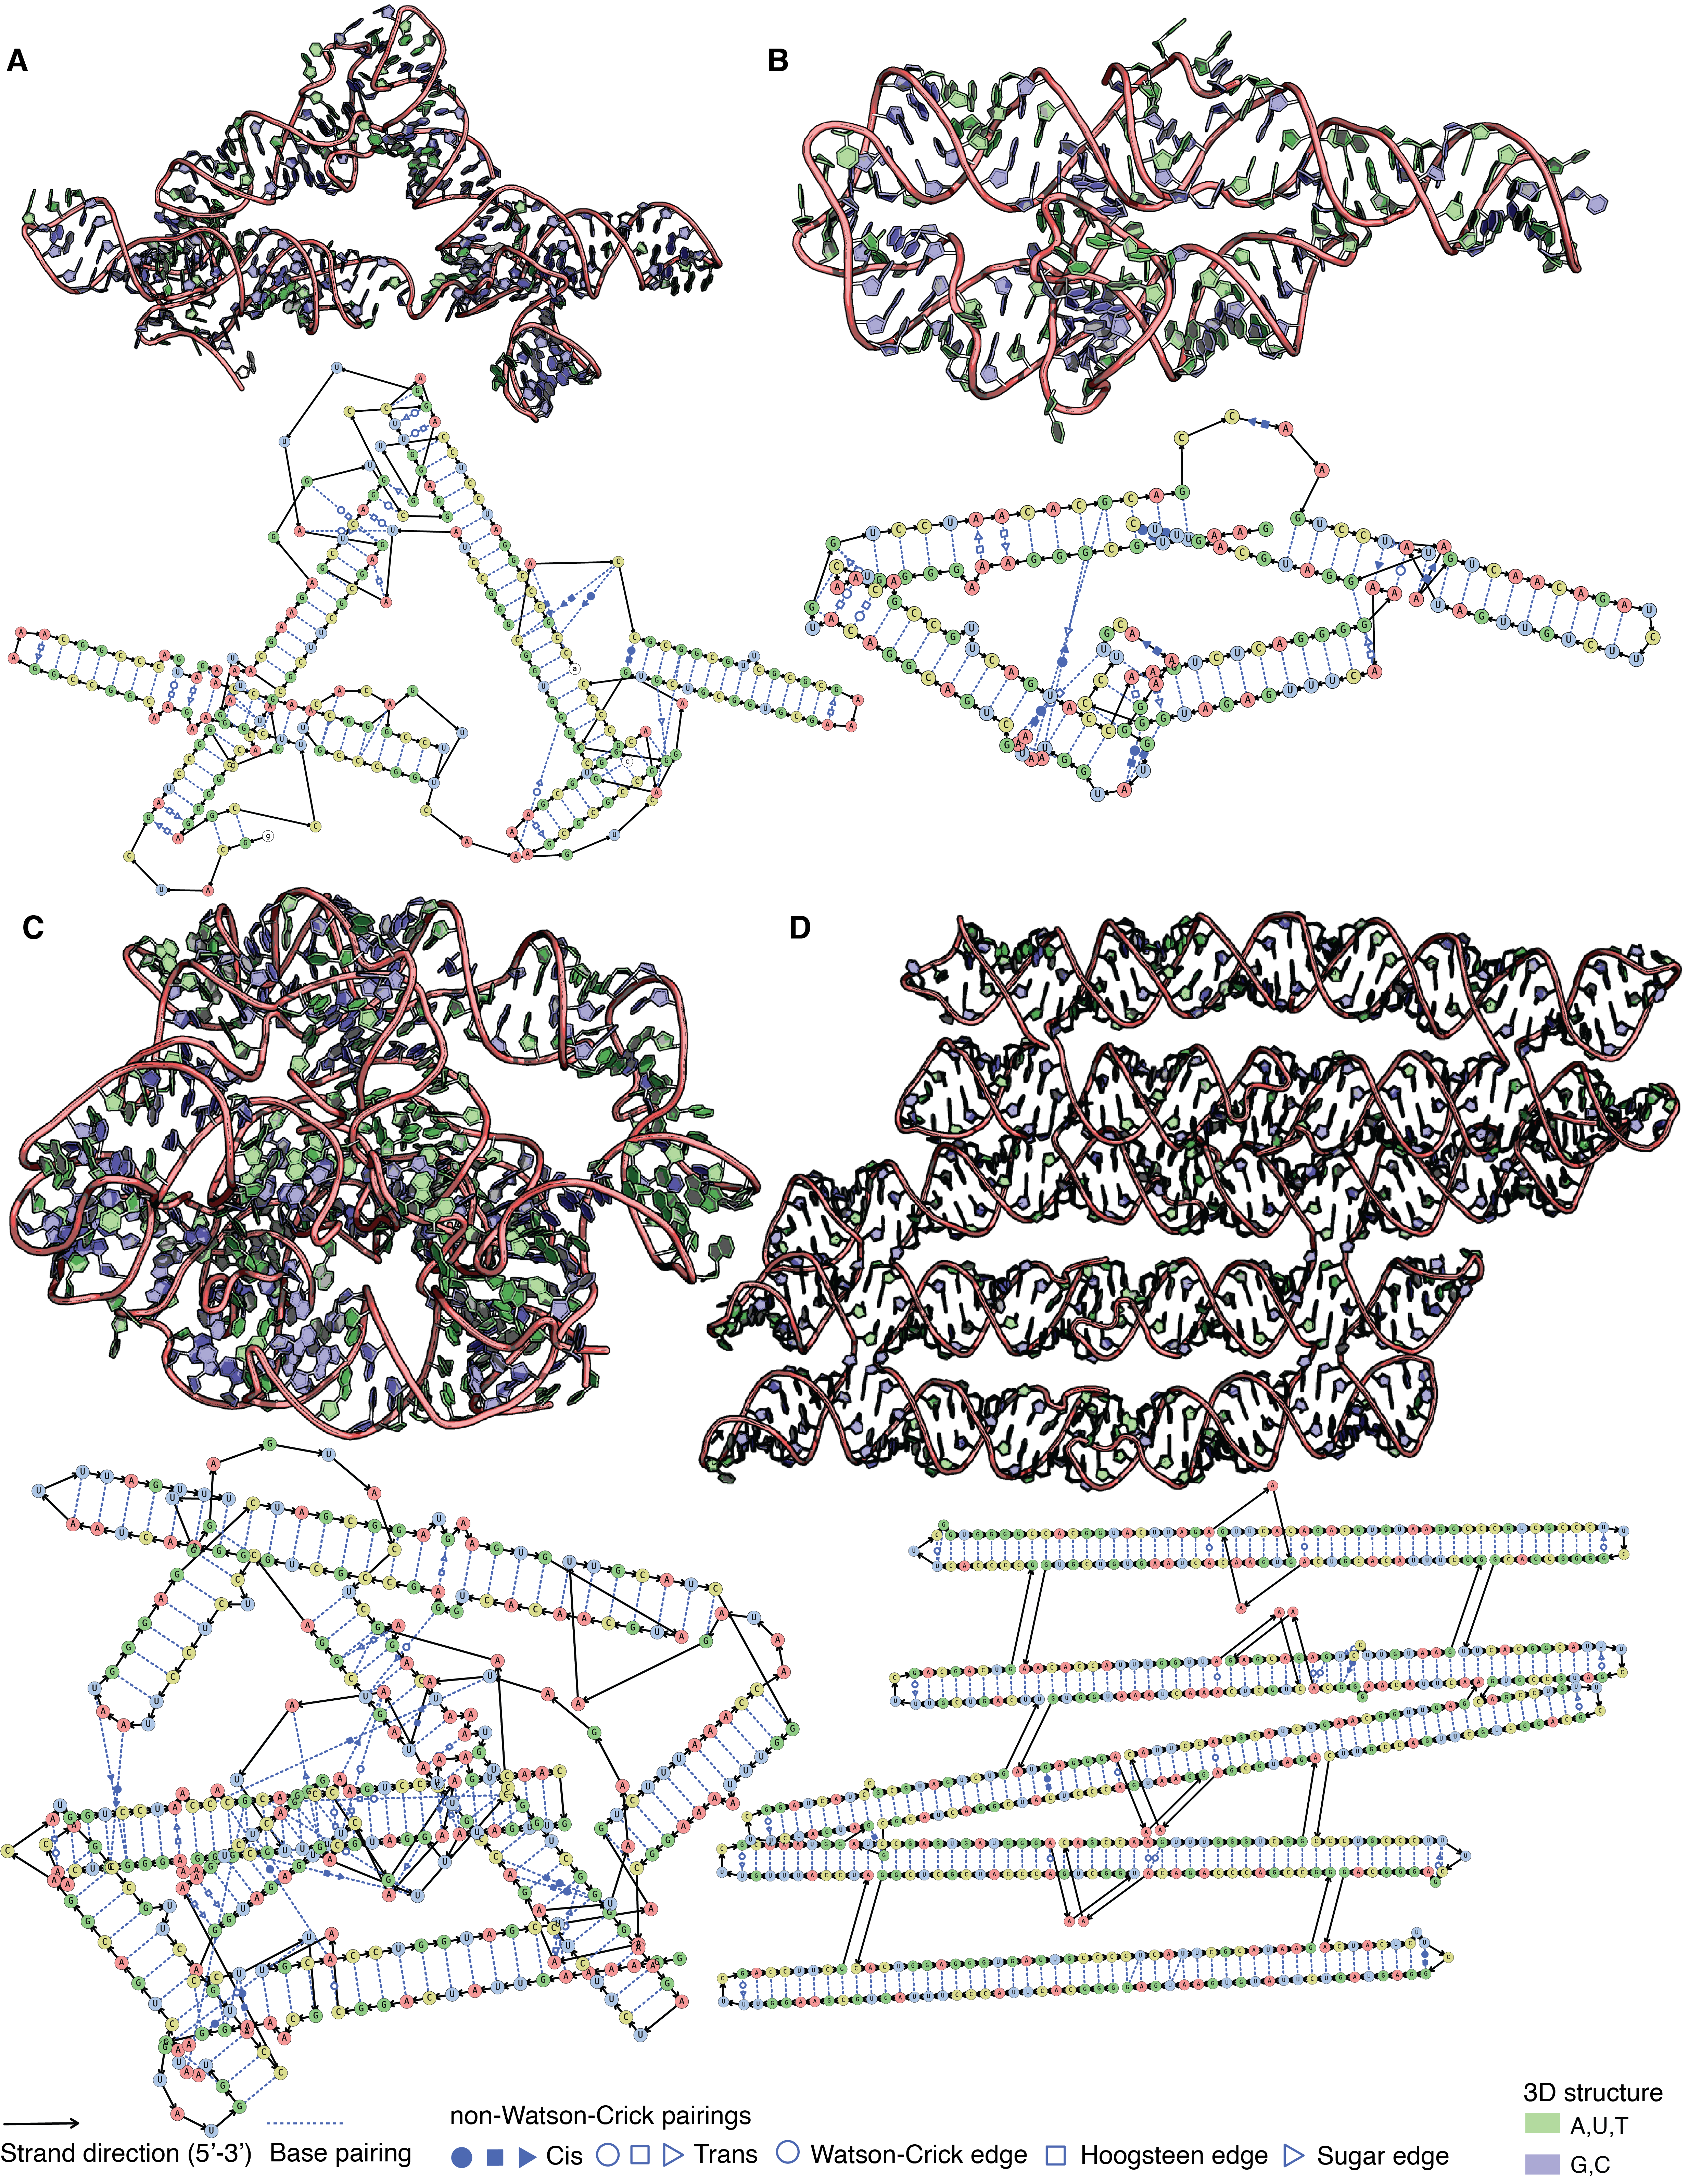
\includegraphics[width=0.7\paperwidth]{./rnascapefigs/figure4.png}}
 % archetecture.png: 1149x508 px, 72dpi, 40.53x17.92 cm, bb=0 0 1149 508
        \caption[Computational cost of training RVAgene]{\textbf{Training RVAgene is reasonably scalable on CPU and even more so using hardware acceleration through GPU.} ({\bf A}) Time cost of training RVAgene for 100 epochs for datasets with varying number of genes and time points on CPU and GPU. ({\bf B}) Maximum memory utilized during training of the model on CPU an GPU for the cases in (A), inset plot: comparison of max memory used compared to DPGP for varying number of genes.}
  \label{fig:rnascape4}
\end{figure}
\end{center}

\section{Discussion}

The RNAscape webserver produces customizable, publication-quality visualizations of nucleic acid tertiary structure. It prioritizes the topology of a structure while striving to create a clean and optimized output, and it is designed to minimize user effort. RNAscape significantly deviates from any existing method in terms of its output quality, usability, and layout algorithm (Supplementary Table S1, Supplementary Figures S1 and S3). Users can refine visualizations on the webserver, and RNAscape also supports non-standard nucleotides and various base-pairing annotations. Further updates to base-pairing conventions may be easily incorporated. The RNAscape webserver allows a maximum file size of 50 MB. While potentially informative, the output for extremely large structures may not be well suited for presentation. We provide the RNAscape implementation via GitHub (see Data Availability) for those inclined to try the pipeline locally on even larger structures. We conclude with the hope that our effort facilitates advancement of the ever-growing field of RNA biology.

%%%%%%%%%%%%%%%%%%%%%%%%%%%%%%%%%%%%%%%%%%%%%%%%%%%%%%%%%%%%%%%%%%%%%%%%%%%%%%%%%%%%%%%%%%%%%%%%%%%%%%%%%%
%%%%%%%%%%%%%%%%%%%%%%%%%%%%%%%%%%%%%%%%%%%%%%%%%%%%%%%%%%%%%%%%%%%%%%%%%%%%%%%%%%%%%%%%%%%%%%%%%%%%%%%%%%%%%%%%%%%%%%%%%%%%%%%%%
\chapter{DNAproDB: an updated database for the automated and interactive analysis of protein–DNA complexes}
\begin{abstract}

DNAproDB (\url{https://dnaprodb.usc.edu/}) is a widely used database, visualization tool, and processing pipeline for analyzing the structural features of protein–DNA interactions. Here we present a substantially updated version through additional data and functionalities. It contains an expanded volume of pre-analyzed protein–DNA structures, which will now be automatically updated weekly. The analysis pipeline now identifies water-mediated hydrogen bonds, and modified visualizations of protein–DNA incorporate this data. Tertiary structure-aware nucleotide layouts are now available. New file formats and external database annotations are supported. The website has been aesthetically modernized, and interactions with graphs and data is more intuitive. We also present a statistical analysis on the updated collection of structures revealing salient patterns in protein–DNA interactions.

\end{abstract}

\section{Introduction}

Protein–DNA interactions play crucial roles in essential cellular functions like gene regulation, genome packaging, and DNA replication \citep{Spitz2012, Lai2017}. Diverse recognition mechanisms underlie these interactions \citep{rohs2009role, Rohs2010, Kitayner2010, Chiu2023}. Atomic resolution structures of protein–DNA complexes available in the Protein Data Bank (PDB) \citep{wwpdb2019protein} have been invaluable for understanding these readout mechanisms and provide insight that relate them to function. As a computational resource which extensively analyzes such structures and presents their data in publication-quality representations, the DNAproDB web server \citep{Sagendorf2017} and database \citep{Sagendorf2020} have been a useful resource for biologists, recognized by tool libraries such as the Nucleic Acid Knowledge Base (NAKB) \citep{Lawson2024}. 
This update improves the DNAproDB analysis pipeline, output data presentation, and web interface \hyperref[fig:dnaprodb1]{Fig. 4.1}. The updated analysis pipeline now computes annotations of water-mediated hydrogen bonds, which are known to play an important role \citep{Reddy2001} in protein–DNA recognition and, in some cases, a very prominent one \citep{Otwinowski1988}. Also, the pipeline now automatically processes and incorporates new PDB structures weekly. The primary interface visualization, ‘Residue contact map,’ now allows users to select a mapping algorithm for nucleic acid layout. In addition to secondary structure-based mapping \citep{Lorenz2011}, tertiary-structure aware mapping \citep{Mitra2024rnascape} is now available. Binding specificity data for transcription factors catalogued in the JASPAR2024 \citep{Rauluseviciute2024} database has been integrated. Users can now upload structures in the macromolecular Crystallographic Information File (mmCIF) format and download interface visualizations in an editable figure format. More information regarding these updates, as well as quality-of-life and user-interface improvements, is described in the following sections.
We analyzed the expanded DNAproDB structure collection for salient features of protein–DNA interactions (\hyperref[fig:dnaprodb2]{Fig. 4.2}). These results (based on a larger sample size in this update) reaffirm previous statistics presented about DNA minor groove recognition \citep{rohs2009role} and patterns of amino acid-base stacking for single stranded DNA presented \citep{Sagendorf2020}. Additionally, we present and discuss examples of the newly added water-mediated hydrogen bond annotations in selected structures (\hyperref[fig:dnaprodb3]{Fig. 4.3}).
DNAproDB has been used by experimental biologists to upload, analyze, and present interface visualizations in their work \citep{Webb2024}. We developed this update to assist their efforts, likely leading to additional contributions from the scientific community. We want to emphasize the increased utility of DNAproDB in light of structure prediction tools like AlphaFold3 \citep{Abramson2024}, RoseTTAFoldNA \citep{baek2024na}, and RoseTTAFold-AA \citep{Krishna2024}, and binding specificity prediction tools including DeepPBS \citep{Mitra2024} and rCLAMPS \citep{Wetzel2022}. These computational tools hint towards a promising future of protein–DNA structure prediction and design \citep{Glasscock2023}. We expect that DNAproDB will be an invaluable tool and assist such efforts.

\begin{center}
    \begin{figure}
    \makebox[\textwidth]{\includegraphics[width=0.8\paperwidth]{./dnaprodbfigs/figure1.png}}
 % archetecture.png: 1149x508 px, 72dpi, 40.53x17.92 cm, bb=0 0 1149 508
        \caption[Key aspects of this update to DNAproDB.]{\textbf{Key aspects of this update to DNAproDB.} ({\bf A}) Automatic update and separated external annotation incorporation scheme.  ({\bf B})  Different nucleic acid layout options in with added tertiary structure aware RNAscape layout, shown for PDB ID: 3LDY. ({\bf C}) Water-mediated hydrogen bond annotation. ({\bf D}) Various improvements in other aspects of DNAproDB. }
  \label{fig:dnaprodb1}
\end{figure}
\end{center}


\section{Update details}

\subsection{Processing pipeline and data update}
At the time of its previous release \citep{Sagendorf2020}, DNAproDB contained a static collection of structures. This resulted in newly released structures being unavailable. In this update, we have addressed this limitation by implementing an automatic update pipeline (\hyperref[fig:dnaprodb1]{Fig. 4.1A}). Every weekend, the pipeline queries the PDB for newly released structures, downloads and processes them, and adds them to the DNAproDB collection. 
In addition, the structure processing pipeline has been separated from any external annotation dependency. This allows external annotations to be updated without reprocessing each structure or affecting the user experience. Annotations from the JASPAR2024 \citep{Rauluseviciute2024} database (incorporating the most recent binding specificity matrix ID and logo) have been included whenever applicable. 
The asymmetric unit molecular weight cutoff, which determines whether a structure is included in the collection, has been expanded from 250 to 1500 kDa, increasing the structures available for analysis. The latest collection size as of June 7th, 2024, is 6,731 structures. This set has been analyzed and was included in the results presented in \hyperref[fig:dnaprodb2]{Fig. 4.2}. 
Originally, a large part of the processing pipeline was written using Python 2 \citep{Guido1995}. However, support for Python 2 is no longer available by the open-source community as of January 1, 2020, and Python 3 \citep{Guido2009} has become the new standard. We redesigned the backend processing pipeline to ensure compatibility with Python 3. 
As an expansion of available features, water-mediated hydrogen bonds between protein and DNA have been calculated and annotated within this update. The program HBPLUS \citep{McDonald1994}, with the ‘-h’ option set to 3 Å, and the ‘-d’ option set to 3.5 Å, and with the remaining parameters set as default, is used to detect hydrogen bonds. Custom scripts were written to determine water-mediated interactions via shared water molecules between hydrogen-bonded pairs (see Data Availability).  

\subsection{Visualization}
We updated the ‘Residue contact map’ and ‘3D structure’ (\hyperref[fig:dnaprodb1]{Fig. 4.1B}) visualizations presented in DNAproDB in several ways. The nucleic acid backbone color used in these components has been changed to a more visually pleasing metallic blue-gray color, compared to the previously used yellow-orange color. 
In addition to the previous secondary-structure-based and circular layouts, an RNAscape \citep{Mitra2024rnascape} based layout for placing nucleic acids has been computed and added to the ‘Residue contact map’. This new layout is more representative of tertiary structure compared to the other two representations (\hyperref[fig:dnaprodb1]{Fig. 4.1B}). An option to switch between these different layouts is available.
During this update, some Python 2 version utilities for secondary structure-based layout computation were discontinued. We replaced these utilities with analogous Python 3 versions provided by the ‘Forgi’ \citep{Thiel2019} package. 
Water-mediated hydrogen bonds have now been incorporated as an interaction edge in the ‘Residue contact map’. These are indicated by a black circle (\hyperref[fig:dnaprodb1]{Fig. 4.1C}) in the interaction map. Hovering over the water-mediated contacts will present further information (e.g., residue number of the water molecule involved). An option to hide these interactions is also available. The ‘3D structure’ component now displays the solvent alongside the structure (in a previous version, the solvent was removed). A button to hide solvent is included. 

\subsection{Web interface and user experience}

Since its inception, we have continuously provided support for DNAproDB users and taken note of their feedback. In this update, we redesigned the web interface based on this information (\hyperref[fig:dnaprodb1]{Fig. 4.1D}). Textual clutter has been reduced on the home page and report pages for each structure. Instructions and explanations for different components, which were previously written directly on the page, are now available as pop-up components upon mouse hover. Report pages for each PDB entry now prominently display the title of the entry. The information tables have been rearranged in a modern and tabular fashion, resulting in further decluttering of information. 
DNAproDB offers many customization features for the Residue contact map. However, these options were often overlooked by users due to their non-prominent placement on the website. We have redesigned the user interface to make basic options like rotation, zooming, download, and switching between the layout algorithms easily accessible directly above the visualization. Buttons to access further customization options (‘Chart options’ and ‘Interface selection’) are prominently placed. The options within the ‘Chart options’ tab have been expanded. Within the ‘Interface selection’ tab, basic options (model, entity, chain, moiety selection) are shown first. Additional options are presented as advanced options. Mouse-based interaction controls for the ‘3D viewer’ and ‘Residue contact map’ have been made analogous, as much as possible.
The download option now supports the editable Scalable Vector Graphics (SVG) format. DNAproDB currently displays Watson-Crick, Hoogsteen, and other base-pairing geometries via correspondingly stylized base-pairing edges (e.g., Hoogsteen base-pairing in p53-tetramer-DNA complex \citep{Kitayner2010} reflected in \hyperref[fig:dnaprodb3]{Fig. 4.3E}). For additional analysis of non-Watson-Crick base-pairing geometries, a link to the RNAscape \citep{Mitra2024rnascape} webserver has been included in each report page. Clicking this link will redirect the user to the RNAscape website and automatically run it on the desired structure.

\subsection{Quantitative analysis of readout features}
Entries in the DNAproDB collection (as of June 7th, 2024) encompass protein–DNA structures including single-stranded (ssDNA), double-stranded DNA (dsDNA), and other conformations (e.g., G-quadruplex). We quantified the growth of such entries over time based on their PDB release dates, which reflects an exponential trend (\hyperref[fig:dnaprodb2]{Fig. 4.2A}). Fewer entries contain ssDNA and other conformations compared to dsDNA. However, recent years (2016 onwards) demonstrate a steady growth also in ssDNA entries (\hyperref[fig:dnaprodb2]{Fig. 4.2A}). 
Studies on protein-DNA structures have revealed consistent patterns in protein residue–DNA interaction frequencies \citep{rohs2009role, Lin2019}. We sought to quantify similar statistics in the updated collection of DNAproDB. To this end, we computed relative abundances of different amino acids interacting with the major groove (\hyperref[fig:dnaprodb2]{Fig. 4.2B}), minor groove (\hyperref[fig:dnaprodb2]{Fig. 4.2C}), and phosphodiester backbone (\hyperref[fig:dnaprodb2]{Fig. 4.2D}). Relative abundance for a residue (R) is the fraction of appearance of this protein residue in an interaction with a DNA moiety relative to other residues. 
\begin{align}
\text{Relative abundance (R)} = \frac{|\text{interactions involving R}|}{\sum\limits_\text{R}|\text{interactions involving R}|}
\end{align}
\begin{center}
    \begin{figure}
    \makebox[\textwidth]{\includegraphics[width=0.8\paperwidth]{./dnaprodbfigs/figure2.png}}
 % archetecture.png: 1149x508 px, 72dpi, 40.53x17.92 cm, bb=0 0 1149 508
        \caption[Quantitative analysis of protein–DNA complexes in the DNAproDB collection. ]{\textbf{Quantitative analysis of protein–DNA complexes in the DNAproDB collection. } ({\bf A}) PDB release years of structures catalogued in the updated DNAproDB collection (as of June 7th, 2024). ({\bf B-D})   Relative abundance of different amino acids interacting with DNA major groove (B), minor groove (C), and phosphodiester backbone (D). ({\bf E}) Conditional probabilities of different protein residues and base forming a stacking geometry. Y-axis represents summed values over the bases for each amino acid.({\bf F-H}) Counts of interactions with different bases, categorized by major and minor groove for secondary structure classes: Helix (includes $\alpha$/$3_{10}$/$\pi$-helix) (F), Sheet ($\beta$-sheet) (G) and loop residues (H) }
  \label{fig:dnaprodb2}
\end{figure}
\end{center}
This is computed separately for the major groove, minor groove, and DNA backbone. Each of these values in \hyperref[fig:dnaprodb2]{Fig. 4.2B-E} is further subdivided into fractions per DNA base, shown in four colors. For the major groove, we see an abundance of residues able to perform recognition via hydrogen bonds with arginine (Arg) and lysine (Lys) residues showing the greatest presence (\hyperref[fig:dnaprodb2]{Fig. 4.2B}). For the minor groove, this preference for arginine and lysine is even stronger relative to other residues (\hyperref[fig:dnaprodb2]{Fig. 4.2C}). This agrees with the observation that the minor groove is more electronegative \citep{rohs2009role}, favoring positively charged amino acid sidechains while repelling negatively charged sidechains (e.g., aspartic acid (Asp), glutamic acid (Glu) etc.). 
For amino acid residues (R) with a planar side chain component (i.e., able to form a stacking interaction with a base (B $\in$ [A,C,G,T]) in single-stranded DNA), interaction geometries (g) can be of three types: g $\in$ [stack, pseudo pair, other]. Stacking conditionals P(g=stack $|$ R, B) were computed for major and minor groove interactions as a fraction of the counts of stack geometry against counts for all geometries. i.e.,
\begin{align}
P(\text{g=stack} | \text{R, B})= \frac{|\text{g=stack, R,B}|}{\sum\limits_\text{g}|\text{g, R, B}| }
\end{align}
This information is presented in \hyperref[fig:dnaprodb2]{Fig. 4.2E} in the form of a stacked bar chart. The total height of each stacked bar (i.e., for each amino acid) is $\sum\limits_\text{B}P(\text{g=stack} | \text{R, B})$ . The pattern visible in this data conforms with the previously computed version in \citep{Sagendorf2020} while encompassing a larger sample size.
DNAproDB also provides annotations and a visualization (‘Helical contact map’) reflecting how various secondary structure elements of a protein interact with the major and minor groove of DNA. We quantified these interactions to reveal statistical patterns (\hyperref[fig:dnaprodb2]{Fig. 4.2F-H}). We compute instances of helical secondary structures (including $\alpha$-helices, $3_{10}$-helices, and $\pi$-helices) interacting with the four primary DNA bases in either the major or minor groove (\hyperref[fig:dnaprodb2]{Fig. 4.2F}). There is a clear preference for the major groove for protein helices, reflecting the use of a recognition helix by many protein families \citep{Garvie2001}. On the other hand, for $\beta$-sheets, major and minor groove interactions are comparable in number, with a slight preference for the major groove (\hyperref[fig:dnaprodb2]{Fig. 4.2G}). The ‘loop’ category reflects residues appearing in loop regions of proteins interacting with DNA. Minor groove interactions are slightly more favored in this case (\hyperref[fig:dnaprodb2]{Fig. 4.2H}). In all cases, guanine (G) is the most favored DNA base that is contacted. 

\subsection{Water-mediated hydrogen bonds}
As described previously, the updated DNAproDB processing pipeline detects and visually annotates (\hyperref[fig:dnaprodb1]{Fig. 4.1B}) water-mediated hydrogen bond interactions between protein and DNA. This feature improves the accuracy and relevance of the DNAproDB visualization for some structures. For example, the co-crystal structure of the Trp repressor/operator complex (PDB ID: 1TRO, \hyperref[fig:dnaprodb3]{Fig. 4.3A}, Residue contact map: \hyperref[fig:dnaprodb3]{Fig. 4.3B}) reflects a protein–DNA recognition scheme without any direct hydrogen bonds in the major and minor groove. Instead, DNA recognition occurs via water-mediated hydrogen bonds (\hyperref[fig:dnaprodb3]{Fig. 4.3B}) \citep{Otwinowski1988}. A detailed view of two protein backbone nitrogen atoms (belonging to Ile79 and Ala80) recognizing G11 in this manner is presented in \hyperref[fig:dnaprodb3]{Fig. 4.3C}. This type of recognition scheme was previously not reflected in DNAproDB. Similarly, protein residues interacting with DNA only through water-mediated hydrogen bonds were also not displayed in the Residue contact map. One such example is the p53 tetramer structure (PDB ID: 3KZ8 \citep{Kitayner2010}, \hyperref[fig:dnaprodb3]{Fig. 4.3D}, Residue contact map: \hyperref[fig:dnaprodb3]{Fig. 4.3E}). This structure illustrates serine residues (Ser121) near the tetramerization interfaces involved in water-mediated hydrogen bonds with the major groove edge of two G bases (shown for one selected base in \hyperref[fig:dnaprodb3]{Fig. 4.3F}). As this is the sole mode of interaction for these two residues, they were omitted from the visualization in the previous DNAproDB version \citep{Sagendorf2020}. In this update, these interactions are correctly shown. A variety of complex interaction geometries are possible when water-mediated hydrogen bonds are involved. One such example can be found in interactions of the RXR/RAR DNA-binding domain heterodimer in complex with the retinoic acid response element (PDB ID: 1DSZ \citep{Rastinejad2000}, \hyperref[fig:dnaprodb3]{Fig. 4.3G}, Residue contact map: \hyperref[fig:dnaprodb3]{Fig. 4.3H}). The lysine residue (Lys1260) is involved in recognizing consecutive bases (G and T) through water-mediated hydrogen bonds involving two different water molecules. This update to DNAproDB allows exploring such recognition schemes. 

\begin{center}
    \begin{figure}
    \makebox[\textwidth]{\includegraphics[width=0.8\paperwidth]{./dnaprodbfigs/figure3.png}}
 % archetecture.png: 1149x508 px, 72dpi, 40.53x17.92 cm, bb=0 0 1149 508
        \caption[Water-mediated hydrogen bond annotation in DNAproDB]{\textbf{Selected examples of water-mediated hydrogen bond annotations as reflected in the updated DNAproDB.  } ({\bf A-C}) Trp repressor/operator complex (PDB ID: 1TRO)  ({\bf D-F})    p53 tetramer with Hoogsteen base pairs (PDB ID: 3KZ8). ({\bf G-I}) Conditional probabilities of different protein residues and base forming a stacking geometry. Y-axis represents summed values over the bases for each amino acid.({\bf F-H}) RXR-RAR DNA-binding complex (PDB ID: 1DSZ). In each of the three cases, the 3D structure of the respective complex is shown in (A, D, G). The DNAproDB Residue contact map is shown (with only selected protein residues annotated) in (B, E, H). Atomic views of selected water-mediated hydrogen bond interactions are shown in (C, F, I), respectively. }
  \label{fig:dnaprodb3}
\end{figure}
\end{center}


\section{Discussion}
DNAproDB, since its inception in 2017 \citep{Sagendorf2017}, has been a valuable resource for the structural biology community. Its unique and extensive analysis pipeline, covering diverse aspects of protein–DNA binding, outputs data that can be readily used in downstream analysis by the user \citep{Sagendorf2020}. The interactive and publication-quality visualizations presented by DNAproDB have been used extensively by the structural biology community. In this update, we improved DNAproDB in multiple aspects. New structures released since the last update in 2019 \citep{Sagendorf2020} have been incorporated, resulting in a much larger collection. The pipeline has been future-proofed via the new automatic update feature. The backend implementation has been upgraded to Python 3, ensuring a long-lasting lifespan for DNAproDB. 
A key scientific improvement in the analysis pipeline is the incorporation of water-mediated hydrogen bond calculation. Interest in water-mediated interactions has been growing. This is evidenced by the CASP16 challenge for predicting solvent shells around the Tetrahymena ribozyme structure \citep{kryshtafovych2023critical}. Currently, these interactions are not well modelled by structure prediction and analysis tools \citep{Abramson2024, baek2024na, Krishna2024, Mitra2024, Jumper2021, Sagendorf2024}. We expect that this added feature in DNAproDB advances the field in the understanding of readout mechanisms. 
Visualizations have been improved by enabling tertiary structure-aware nucleic acid layouts, incorporation of water-mediated hydrogen bond indicators, greater customizability, and other aesthetic changes. The website style has been redesigned, and data presentation has been improved. Structure files in mmCIF format can now be uploaded, which was previously unsupported. Altogether, these updates result in an updated DNAproDB, which we expect to continue serving the structural biology community for the foreseeable future.

\subsection{Data availability}
DNAproDB is freely available for all users at \url{https://dnaprosb.usc.edu/}. The previous version remains available at \url{https://dnaprosb.usc.edu/v1/}. 
The pipeline and frontend implementations are available via GitHub:
\url{https://github.com/timkartar/DNAproDB}; 
\url{https://github.com/ariscohen/DNAproDB_frontend}

%\section{Introduction} 

The structural diversity of RNA molecules influences their broad biological functions \citep{Tomezsko2020, seemann2017identification, Mortimer2014}. This diversity \citep{Batey1999} is primarily driven by its ability to form complicated tertiary interactions, a plethora of non-standard base-pairing conformations and quaternary interactions with other RNA, DNA or protein molecules. Visualizing RNA in two dimensions poses the challenge of capturing these complex interactions while remaining comprehensible and valuable to researchers.
\par
One popular means of representing complicated RNA structures is through secondary structure diagrams. These two-dimensional (2D) diagrams are exclusively driven by base-pairing relationships and laid out in an abstract space. Extensive literature and software \citep{Johnson2023, Sweeney2021,Weinberg2011,Wiegreffe2019,Shabash2019,Peter2003,Byun2009,Darty2009,Kerpedjiev2015,Lu2018,Waterman1978} describe secondary structure diagrams. However, these representations do not effectively capture tertiary molecular interactions, such as base pairing, stacking, and pseudoknot interactions. Therefore, although this approach scales relatively well for large RNA sequences \citep{Johnson2023}, not considering tertiary interactions can lead to a diagram far from the biological structure and function. More specifically, nucleotides which are positioned relatively close together in three-dimensional (3D) space may appear far away in the visualization.
\par
Some tools promise to capture tertiary interactions \citep{Yang2003,Mallet2022}. Of these tools, RNAView \citep{Yang2003}, is widely known and has been a current standard linked in the Nucleic Acid Knowledge Base (NAKB) \citep{Lawson2024}. However, RNAView \citep{Yang2003} lacks a webserver, requires a complicated setup and usage pipeline, and cannot handle some complex topologies resulting in output that is not always interpretable or intuitive. Moreover, it is unable to provide publication-quality images. The only other available tool that retains tertiary interactions, RNAglib \citep{Mallet2022}, is not deterministic and results in different outputs for repeat runs under the default configuration documented by the authors, which likely explains why it has not been adopted by the field compared to RNAView. A description of different tools which create various 2D diagrams of RNA molecules is provided in \hyperref[table:rnascape]{Table 3.1}.
\par
RNAscape addresses and overcomes the outlined issues and limitations of existing approaches at several levels. The RNAscape algorithm includes a mapping process that conforms to the helical geometry of RNA structures. By doing so, it attempts to preserve the intuitive correspondence between the 2D mapping and 3D structure. At the same time, RNAscape optimizes each layout to place non-helical segments of the structure without sacrificing tertiary interactions. This enables visualizations that are compact while remaining as visually intuitive as possible (Figure 1, Supplementary Figures S1 and S3).
RNAscape output for various structures from the PDB. The 3D structure at the top of each panel is from the PDB structure, with its corresponding RNAscape visualization shown below it. (A) tRNA from Sulfolobus tokodaii (PDB ID: 7VNV), (B) a single-stranded DNA molecule (PDB ID: 4NOE), (C) Dengue virus RNA promoter (PDB ID: 7UMD), (D) Pistol ribozyme (PDB ID: 6R47), (E) Riboswitch from Escherichia coli (PDB ID: 1Y26), (F) Cobalamin riboswitch regulatory element (PDB ID: 4FRN), (G) NAD-II riboswitch (PDB ID: 8HBA), (H) G-quadruplex (PDB ID: 2M18), (I) RNA kink-turn motif (PDB ID: 7EFG) and (J) the semi-symmetric peptidyl transferase center (PTC) of the large ribosomal subunit of Deinococcus radiodurans (PDB ID: 1NKW), also known as proto-ribosome (30). The molecular structure in (J) is shown along the two-fold pseudo-symmetry axis, with an additional orientation shown in Supplementary Figure S1.
\par
The RNAscape webserver (Figure 2) offers various customization options for its visualizations. Users can zoom, pan, and rotate images directly on the webserver. In addition, one can easily customize a plot with different base-pairing annotations \citep{Yang2003, Saenger1984,lu2015dssr}, residue colors, nucleotide or text-label sizes, and numbering schemas. RNAscape encourages users to iteratively refine an image. In addition, RNAscape allows the user to modify the calculated map. Upon completion, RNAscape visualizations can be exported to vector format (SVG) or image format (PNG), enabling further refinements by the user. Both Protein Data Bank (PDB) and macromolecular Crystallographic Information File (mmCIF) format files are supported to maximize compatibility. Additionally, RNAscape can directly fetch structures (biological assembly 1) from the PDB \citep{berman2000protein,} based on a given PDB ID. RNAscape supports multiple base-pairing annotation conventions: Leontis-Westhof (LW) \citep{Yang2003}, Saenger \citep{Saenger1984}, DSSR (Dissecting the Spatial Structure of RNA) \citep{lu2015dssr} and a no-annotation option. Future updates to base-pairing conventions by the nucleic acid community can easily be incorporated. Modified/non-standard nucleotides are denoted by a white circle and annotated with a small letter code (based on its parent standard base or simply ‘x’ if this information is unavailable).
\begin{center}
    \begin{figure}
    \makebox[\textwidth]{\includegraphics[width=0.8\paperwidth]{./rnascapefigs/figure1.png}}
 % archetecture.png: 1149x508 px, 72dpi, 40.53x17.92 cm, bb=0 0 1149 508
        \caption[RNAscape output for various structures from the PDB.]{\textbf{RNAscape output for various structures from the PDB.} The 3D structure at the top of each panel is from the PDB structure, with its corresponding RNAscape visualization shown below it. ({\bf A}) tRNA from Sulfolobus tokodaii (PDB ID: 7VNV), ({\bf B}) a single-stranded DNA molecule (PDB ID: 4NOE), ({\bf C}) Dengue virus RNA promoter (PDB ID: 7UMD), ({\bf D}) Pistol ribozyme (PDB ID: 6R47), ({\bf E}) Riboswitch from Escherichia coli (PDB ID: 1Y26), ({\bf F}) Cobalamin riboswitch regulatory element (PDB ID: 4FRN), ({\bf G}) NAD-II riboswitch (PDB ID: 8HBA), ({\bf H}) G-quadruplex (PDB ID: 2M18), ({\bf I}) RNA kink-turn motif (PDB ID: 7EFG) and ({\bf J}) the semi-symmetric peptidyl transferase center (PTC) of the large ribosomal subunit of Deinococcus radiodurans (PDB ID: 1NKW), also known as proto-ribosome (30). The molecular structure in (J) is shown along the two-fold pseudo-symmetry axis.}
  \label{fig:rnascape1}
\end{figure}
\end{center}

%\section{Materials and methods} 

\subsection{Programming languages and general tools}

The RNAscape webserver is a single-page web application. The backend (Figure 2A, B) is implemented in Python 3.9.18, and Django \citep{Django2019} is used to communicate with the backend. The frontend is (Figure 2C) designed in React v18.2.0 framework and implemented in Hypertext Markup Language (HTML)/Cascading Style Sheets (CSS)/JavaScript.

\subsection{The RNAscape algorithm}

Upon upload, the structure file is sent via Hypertext Transfer Protocol Secure (HTTPS) to the RNAscape webserver where backend processing occurs. If a user selects a PDB ID \citep{berman2000protein}, its corresponding first biological assembly is downloaded by the backend (Figure 2A, B) for processing.

Pre-processing (Figure 3A). The DSSR program (v1.7.8) \citep{lu2015dssr} is run on the structure file to detect helices and base pairs, and assign base-pairing annotations.

Helical regions (Figure 3B). The positioning of helices, as well as non-helical regions, involves multiple considerations. The 3D coordinates of each nucleotide are represented by the centroid of atoms belonging to it (i.e. for the nucleotide,
). The set of all nucleotide centroids is a combination of two subsets (i.e. (helical regions) and (non-helical regions)). Helical regions receive the highest priority and are placed in a way that reflects their spatial orientation while remaining visually intuitive. To do so, first, we run principal component analysis (PCA) exclusively on the helical segments () and project the points onto the plane determined by the first two components. In this process, the  sized matrix is converted to a matrix (which we can denote as ), which preserves the maximum spatial variance possible in two dimensions \citep{Pearson1901}. Next, we convert into a more visually intuitive ‘ladder’ representation, which first involves estimating a ladder axis in the projection plane for each helix. An initial estimate is made by connecting the centroid of the first and last base pairs of a helical region using a line segment. consists of multiple helical regions (i.e. ). If the midpoint of a base-pair is
, the ladder axis for is the vector
rooted at the point

.

However, for bent helices, this estimate may be imprecise. To account for this case, we measure the distance
 between the centroid of the helical projection and the midpoint of the estimated ladder axis (i.e.
. If this distance is greater than 10 Å, we re-estimate the ladder axis as a combination of two line segments: one connecting the first and central base-pair centroids and another between the central and last base-pair centroids. In theory, this process can be recursively performed. In practice, however, we observe that doing so once suffices. Next, if two helical projections are within a certain distance threshold (i.e.
Å) and have similar orientations (i.e.
), we merge them and recompute the ladder axis as described above. Next, we uniformly distribute the base pairs in the ‘ladder’ formation along each ladder axis. Finally, for cases where the projection of a helix is skewed, resulting in an overly cramped ladder representation, we lengthen the ladder to reduce visual clutter. The final mapping for nucleotide points in helical regions can be denoted as Non-helical regions (Figure 3C). Loops are either preferentially bulged out in a radial curve or interpolated linearly based on a spatial density threshold (see implementation in Data Availability), depending on the chosen setting. We choose bulging by default to reduce graph overlap and crowding. For bulging out, the structure mapping algorithm computes potential layouts and performs greedy optimization to select an optimal layout. This optimization considers the total nearest-neighbor count (within 10 Å) of all members of a loop, and the orientation with the lowest number of neighbors is selected. Let us assume that the loop is connected to two nucleotides which are part of a helical region, mapped to positions
. Two possible circular layouts are computed for the loop based on
and
: bulging out in perpendicular directions
(layout ) and
(layout ), where
denotes the unit vector which is perpendicular relative to the mapping plane. In each case, the center of the layout remains at the point (
. The radius of the circular arc is either 
, if
 \AA or
 \AA, where

is the number of points in the loop. Points are uniformly distributed on the circular arc. One of the two loop orientations is selected based on minimizing the neighbor count in helical segments as follows:

Hanging single stranded regions are linearly interpolated based on its connecting mapped helix. Additional adjustments are made for certain edge cases, such as, when a linearly interpolated non-helix nucleotide exactly overlaps with another nucleotide (see implementation in Data Availability). Structures containing no helices (generally rare) are mapped solely using a PCA.

Visualization (Figure 3C). The RNAscape backend utilizes the Matplotlib \citep{Hunter2007,} and NetworkX \citep{Hagberg2008} packages to plot visualizations. As input, the plotting algorithm requires the mapped points, base-pairing annotations, and user-selected visual settings for a structure. As output, it generates an image that is temporarily stored (up to 48 h) on the webserver and tied to a specific user session. Structure files are not stored. The image is served to the frontend via a Django \citep{Django2019} server, where it can be interacted with by the user. A user can also regenerate a plot with different visual settings. In this case, we reuse the mapping output and rerun the visualization script, resulting in a faster response time than the complete computation.
\begin{center}
    \begin{figure}
    \makebox[\textwidth]{\includegraphics[width=0.8\paperwidth]{./rnascapefigs/figure2.png}}
 % archetecture.png: 1149x508 px, 72dpi, 40.53x17.92 cm, bb=0 0 1149 508
        \caption[Computational cost of training RVAgene]{\textbf{Training RVAgene is reasonably scalable on CPU and even more so using hardware acceleration through GPU.} ({\bf A}) Time cost of training RVAgene for 100 epochs for datasets with varying number of genes and time points on CPU and GPU. ({\bf B}) Maximum memory utilized during training of the model on CPU an GPU for the cases in (A), inset plot: comparison of max memory used compared to DPGP for varying number of genes.}
  \label{fig:rnascape2}
\end{figure}
\end{center}

%\section{Results}
\subsection{Application of RNAscape to structures from the PDB}

We present RNAscape output for various structures (Figures 1 and 4) from the PDB (21). In Figure 1A, tRNA from Sulfolobus tokodaii (PDB ID: 7VNV) is shown. RNAscape output preserves the L-shaped topology (as opposed to known ‘clover leaf’ shaped secondary structure (26) visualizations) and annotates non-standard bases and base-pairing geometries (critical in many RNA interactions (27)). RNAscape can also process unusual DNA structures, as shown by a single-stranded DNA with circular topology (PDB ID: 4NOE, Figure 1B). In Figure 1C, Dengue virus RNA promoter (PDB ID: 7UMD) is depicted, which is a single-stranded RNA molecule containing only standard RNA bases.

We present a few different examples of ribozymes and riboswitches (Figure 1D-G). RNA loop modeling (28) for riboswitches is an important area of research, and RNAscape visualizations (e.g. PDB IDs: 1Y26, 4FRN, 8HBA, Figure 1E-G) may aid in these efforts. The pistol ribozyme (PDB ID: 6R47, Figure 1D) and the Nicotinamide Adenine Dinucleotide-II (NAD-II) riboswitch (PDB ID: 8HBA, Figure 1G) illustrate how RNAscape places non-helical segments and can clearly depict their non-standard base pairs with helical segments. RNAscape natively supports multiple strands (e.g. PDB ID: 1Y26, Figure 1E). RNAscape is also able to visualize G-quadruplexes (PDB ID: 2M18, Figure 1E). An RNA structural motif which can serve as a binding site for proteins is the kink-turn motif (PDB ID: 7EFG) (29), and it is visualized in Figure 1I.

There has been a continued interest in structural studies of the ribosome which postulate the role of a proto-ribosome (30) in the origin of life. The proto-ribosome is a semi-symmetrical core of the ribosome comprised of RNA molecules representing the site for peptide bond formation, therefore known as peptidyl transferase center (PTC). The RNAscape visualization (Figure 1J, Supplementary Figure S1) for the same reflects the high degree of conformational symmetry, based on structural coordinates of the PTC provided by Bose et al. (30).

RNAscape can run on relatively large structures (structures of up to 50 MB are processed by the webserver). In Figure 4, we demonstrate its application to four different topologies of larger structures. In Figure 4A, a triangular topology of Mycobacterium tuberculosis ileS T-box in complex with tRNA (PDB ID: 6UFH, 244 nucleotides) is shown, followed by a diamond-like topology of mutant P4-P6 domain of Tetrahymena thermophila group I intron (PDB ID: 1HR2, Figure 4B, 157 nucleotides) and an exon free state of the Tetrahymena group I intron (PDB ID: 7R6N, Figure 4C, 354 nucleotides). Secondary structure representations will not resemble the structure at all for many of these cases (e.g. stacked ladders, PDB ID: 7QDU, Figure 4D, 552 nucleotides), while RNAscape is able to reflect the 3D topology of these large RNA molecules.
\begin{center}
    \begin{figure}
    \makebox[\textwidth]{\includegraphics[width=0.8\paperwidth]{./rnascapefigs/figure3.png}}
 % archetecture.png: 1149x508 px, 72dpi, 40.53x17.92 cm, bb=0 0 1149 508
        \caption[Computational cost of training RVAgene]{\textbf{Training RVAgene is reasonably scalable on CPU and even more so using hardware acceleration through GPU.} ({\bf A}) Time cost of training RVAgene for 100 epochs for datasets with varying number of genes and time points on CPU and GPU. ({\bf B}) Maximum memory utilized during training of the model on CPU an GPU for the cases in (A), inset plot: comparison of max memory used compared to DPGP for varying number of genes.}
  \label{fig:rnascape3}
\end{figure}
\end{center}
\subsection{RNAscape user interface}

The RNAscape webserver (Figure 2C) displays three primary items: header, file upload, and documentation panels. In the header, a user can click the ‘Run on Example Data’ button to view an example visualization (PDB ID: 3ZP8). In the file upload panel, a user can upload a structure using the file upload feature. This file may contain non-nucleic acid entities which will be ignored. Alternatively, a user can directly input a PDB ID to load its corresponding first assembly file. Clicking the ‘Run’ button runs the RNAscape pipeline on the uploaded structure file or provided PDB ID (biological assembly 1). After running RNAscape for a structure, a user has the option to add a second structure for side-by-side viewing. We demonstrate this capability for two structures of tRNA molecules (PDB IDs: 8UPT and 8UPY, Supplementary Figure S2), introduced by recent work (31) on the importance of tRNA shape. The documentation panel enables easy navigation and provides a quick start guide, tips, and examples for using RNAscape. It also includes detailed explanations for configurable settings.

\subsection{Output images}

The frontend (Figure 2C) natively supports touch-screen compatible image exploration. A user can zoom, center, or reset any zooming/panning via buttons above the display box. The image can also be rotated using a slider, and a ‘regenerate’ button is offered that replots the image, associated annotations, and user customizations in the desired rotation. To the right of the image, a legend is displayed that corresponds to the base-pairing annotation selected by the user. For the Saenger (19) base-pairing annotation, no legend is shown. The local strand direction ($5'$ to $3'$) is indicated by the black arrows between nucleotides for all plots. Other interactions are shown in blue dotted lines. These colors are fully customizable by the user. The user also has the option of downloading RNAscape mapped points in a numerical format (.npz) processable by the NumPy (32) library. Additionally, a log is provided which contains a description of the non-standard/modified nucleotides in the plot and other associated information.

\subsection{Base-pairing annotations}

RNAscape offers three base-pairing annotation styles: LW (16,33), DSSR (20) and Saenger (19). All base-pairing annotations are calculated via DSSR, although any future updates to these conventions by the nucleic acid community can be easily incorporated. Annotations do not affect geometric mapping, and a user can forego an annotation altogether. The LW annotation contains two key parameters: bond orientation (cis/trans) and base edge type. Bond orientation is represented by a filled or unfilled marker. The edge types: Watson-Crick (W), Hoogsteen (H), or sugar (S), are represented by marker shapes (Figure 1).

The DSSR style differs in that base edges are delineated by major groove (M), minor groove (m), or Watson-Crick (W) edges. Bond orientation annotation is the same as in the LW (16,33) annotation. DSSR also reports local strand orientation as a base-pairing annotation feature. RNAscape always denotes local strand orientation by the backbone arrows (Figure 1). Non-standard pairings flagged as ‘not categorized’ by DSSR are not annotated. For the Saenger (19) annotation, each bond type is represented by a number corresponding to its Roman numeral annotation.

\subsection{Customizable settings}

Several custom settings options are available (Figure 2C). The Loop Bulging setting controls whether loops are bulged outwards or linearly interpolated (see Materials and Methods). Additionally, the post-processing step of merging proximate, similarly oriented ladders can be turned off (Figure 3B). Since these settings affect the geometric mapping, a user must click ‘Run’ to run the pipeline again if they are changed. Arrow size, circle size, and circle label size affect nucleotide appearance. Base-pairing marker sizes can also be adjusted. Through the number settings, a user instructs RNAscape to label residue numbers in the numbering schema defined by the structure file. Color, size, frequency, and spacing of these labels can also be modified. Color settings allow a user to customize the color of each nucleotide type: A, C, G, U/T and X (non-standard nucleotides). Colors used to denote both backbone chain and non-chain interactions and markers can also be modified. Furthermore, RNAscape provides a functionality to modify calculated maps. By clicking on the ‘Modify Mapping’ button, the user can move and adjust nucleotide locations to resolve, for instance, overlap and regenerate the output.
\begin{center}
    \begin{figure}
    \makebox[\textwidth]{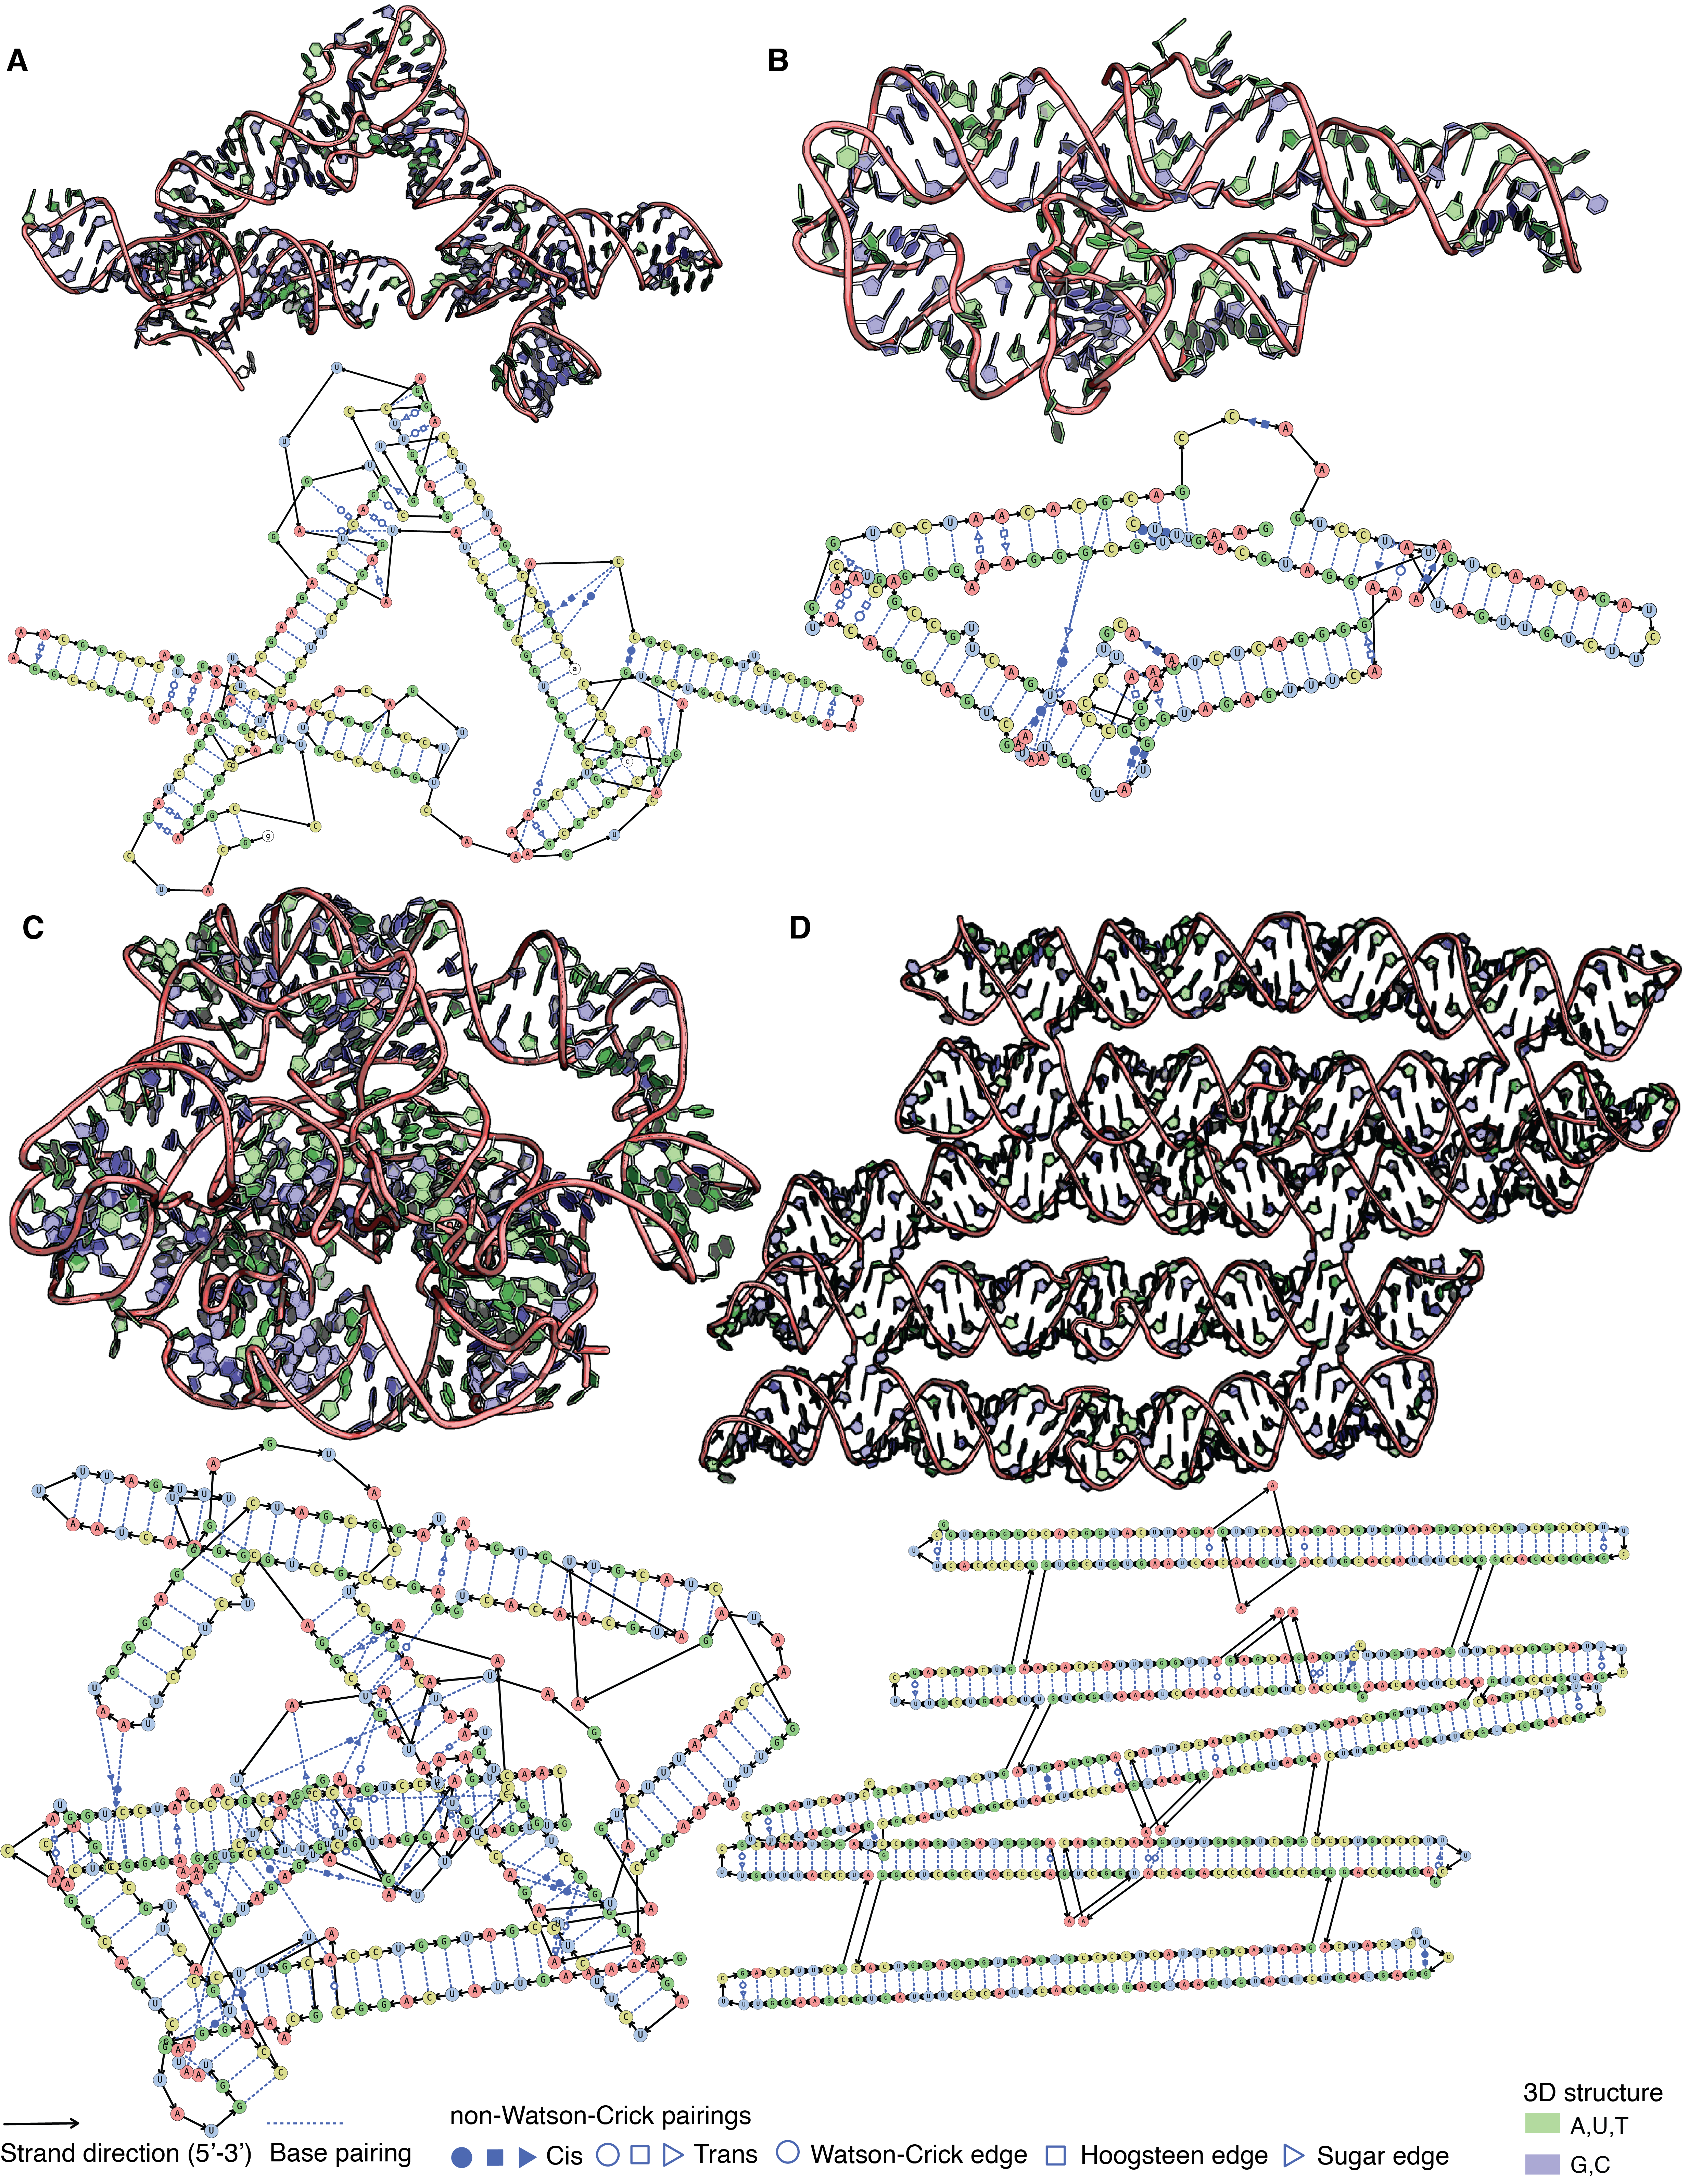
\includegraphics[width=0.7\paperwidth]{./rnascapefigs/figure4.png}}
 % archetecture.png: 1149x508 px, 72dpi, 40.53x17.92 cm, bb=0 0 1149 508
        \caption[Computational cost of training RVAgene]{\textbf{Training RVAgene is reasonably scalable on CPU and even more so using hardware acceleration through GPU.} ({\bf A}) Time cost of training RVAgene for 100 epochs for datasets with varying number of genes and time points on CPU and GPU. ({\bf B}) Maximum memory utilized during training of the model on CPU an GPU for the cases in (A), inset plot: comparison of max memory used compared to DPGP for varying number of genes.}
  \label{fig:rnascape4}
\end{figure}
\end{center}

\section{Discussion}

The RNAscape webserver produces customizable, publication-quality visualizations of nucleic acid tertiary structure. It prioritizes the topology of a structure while striving to create a clean and optimized output, and it is designed to minimize user effort. RNAscape significantly deviates from any existing method in terms of its output quality, usability, and layout algorithm (Supplementary Table S1, Supplementary Figures S1 and S3). Users can refine visualizations on the webserver, and RNAscape also supports non-standard nucleotides and various base-pairing annotations. Further updates to base-pairing conventions may be easily incorporated. The RNAscape webserver allows a maximum file size of 50 MB. While potentially informative, the output for extremely large structures may not be well suited for presentation. We provide the RNAscape implementation via GitHub (see Data Availability) for those inclined to try the pipeline locally on even larger structures. We conclude with the hope that our effort facilitates advancement of the ever-growing field of RNA biology.

%%%%%%%%%%%%%%%%%%%%%%%%%%%%%%%%%%%%%%%%%%%%%%%%%%%%%%%%%%%%%%%%%%%%%%%%%%%%%%%%%%%%%%%%%%%%%%%%%%%%%%%%%%
\chapter{RNAproDB: a webserver and interactive database for analyzing protein–RNA interactions}
\section{Introduction}
Structural complexity of RNA molecules is vast and so are their modes of interaction with proteins \citep{jones2001protein}. Although there has been an ever-expanding repertoire of structural data on the PDB, there is a lack of data resources which systematically analyze these interactions. In addition, recent advances in artificial intelligence have made high throughput prediction of protein-RNA complex structures viable \citep{Abramson2024, watson2023novo}. RNAproDB is a webserver where a user can upload a protein-RNA complex and explore analyzed results covering a multitude of aspects (e.g., direct and water-mediated hydrogen bonds, base-pairing annotations, nucleotide modifications, secondary structural features). Compared to existing resources, which often focus on the RNA structure alone and provide a particular way of visualization \citep{Kerpedjiev2015, Yang2003}, or use a representation which is very coarse-grained \citep{chojnowski2014rna}, RNAproDB provides three different algorithms for visualizing the RNA topology along with the interacting protein residues: a new design based on partial projection of the structure (RNA and interacting protein residues), tertiary structure aware mapping \citep{Mitra2024rnascape}, secondary structure-based mapping \citep{Kerpedjiev2015}. This information is presented via a highly interactive interface explorer combined with sequence and 3D-structure viewers, and a secondary structure selector. Tabular data is also available. Another novel functionality, subgraph exploration, allows a user to explore parts of the structure (e.g., a particular junction region) via the interface explorer. Subgraph selections can be manually entered or automatically selected from the secondary structure selector. As of our knowledge, no existing tool offers such capability. In addition to the webserver, we offer pre-analyzed structures containing RNA, from the PDB, in the form of a searchable collection. With a cutoff of 10,000 monomers per biological assembly and molecular weight cut off of 800 kDa on the asymmetric unit, the initial collection of RNAproDB provides around 3,500 biological assemblies containing RNA molecules. RNAproDB will be automatically updated weekly with new PDB entries. We believe RNAproDB will be a valuable resource for the scientific community interested in RNA biology, protein-nucleic acid interaction and function, structure prediction, and drug design.

\begin{center}
    \begin{figure}
    \makebox[\textwidth]{\includegraphics[width=0.8\paperwidth]{./rnaprodbfigs/fig1.png}}
 % archetecture.png: 1149x508 px, 72dpi, 40.53x17.92 cm, bb=0 0 1149 508
        \caption[Key aspects of this update to DNAproDB.]{\textbf{Key aspects of this update to DNAproDB.} ({\bf A}) Automatic update and separated external annotation incorporation scheme.  ({\bf B})  Different nucleic acid layout options in with added tertiary structure aware RNAscape layout, shown for PDB ID: 3LDY. ({\bf C}) Water-mediated hydrogen bond annotation. ({\bf D}) Various improvements in other aspects of DNAproDB. }
  \label{fig:rnaprodb1}
\end{figure}
\end{center}

\section{Processing pipeline}
The RNAproDB processing pipeline starts with a structure and computes multiple visualizations and interaction information from it. As part of the processing piepline multiple softwares are run, which include X3DNA-DSSR (\citep{Lu2015}computes base-pairing geometries, protein-RNA hydrogen bonds and RNA secondary structure), HBPLUS (McDonald1994to compute hydrogen bonds involving water molecules), RNAscape (\citep{Mitra2024rnascape} tertiary structure aware nucleotide mapping), ViennaRNA (\citep{Lorenz2011} secondary structure-based nucleotide mapping), DSSP (\citep{joosten2010series, kabsch1983dictionary} computes protein secondary structure). In addition, custom code has been developed to compute a new ``Partial Projection" based mapping for the nucleotides. The processing piepleine combines all these data into a graph object which is used to compute highly interactive frontend presentation of the structure. This frontend presentation is an intertwined experience of an Interface Explorer, a 3D Viewer, a secondary structure selector, a Sequence viewer and Tabular data. In the next sections we describe the functionalities implemented through these components.

\section{Interface explorer}

The 'Interface explorer' for RNAproDB is freshly designed to present an interaction graph of the RNA structure along with interacting protein residues. The explorer present three different layout algorithm options, selectable by the user. two of these options are secondary structure based (computed using ViennaRNA \citep{Lorenz2011}) and tertiary structure aware mapping based (computed using RNAscape \citep{Mitra2024rnascape}). The third (default) option is a new mapping scheme produced by prjecting the RNA residues and only interacting protein residues into the 2D plane maximizing their spatial variance \citep{Pearson1901}. We call this method ``Partial projection" (instead of the whole structure, it only projects the RNA and interacting protein components). In our observation, this scheme is visually intuitive for exploring corresponding 3D structure. The user is free to choose between the three layouts. In each case, the protein residues are placed using a force directed layout scheme \citep{bostock2012fl}. We demonstrate the three layout schemes for a valyl-tRNA synthetase-tRNA complex (PDB ID: 1IVS) (\blue{Fig. \ref{fig:rnaprodb1}A}). The partial projection-based layout is shown in \blue{Fig. \ref{fig:rnaprodb1}B}. This layout reflects the helical turns, making the best coreespondance with the 3D structure. The RNAscape \citep{Mitra2024rnascape} layout (\blue{Fig. \ref{fig:rnaprodb1}C}) is cleaner and more suitable for users used to a ladder-like representation.  The secondary structure based layout, shown in \blue{Fig. \ref{fig:rnaprodb1}D}, although familiar, suffers from tertiary interactions within RNA and protein-RNA interactions criss-crossing the view. Options to turn off tertiary interaction edges and protein interactions have been implemented to help with this situation, in case a user wants a clean view of the secondary structure. This is demonstrated in \blue{Fig. \ref{fig:rnaprodb2}A-C}). Another useful feature of the interface explorer is the ability to change distance theshold of visible protein-RNA interactions on the fly. This threshold can be modified using a slider, and upon modification, edge distances that fall beyond the threshold are hidden. At any point of the exploration, the user is able to download the visualization as a static picture, a scalable vector graphic format image or download the corresponding graphical data.


\begin{center}
    \begin{figure}
    \makebox[\textwidth]{\includegraphics[width=0.8\paperwidth]{./rnaprodbfigs/fig2.png}}
 % archetecture.png: 1149x508 px, 72dpi, 40.53x17.92 cm, bb=0 0 1149 508
        \caption[Key aspects of this update to DNAproDB.]{\textbf{Key aspects of this update to DNAproDB.} ({\bf A}) Automatic update and separated external annotation incorporation scheme.  ({\bf B})  Different nucleic acid layout options in with added tertiary structure aware RNAscape layout, shown for PDB ID: 3LDY. ({\bf C}) Water-mediated hydrogen bond annotation. ({\bf D}) Various improvements in other aspects of DNAproDB. }
  \label{fig:rnaprodb2}
\end{figure}
\end{center}
\section{Secondary structure selector and subgraph exploration}

A more coarse grained diagram is also computed as part of the processing piepline for RNAproDB. This diagram reflects the different secondary structure elements as one node each, interaction edges corresponding to residues involved in one secondary structure element with another are collapsed into one edge. This view is presented to serve as a selectable by the user, named "Secondary structure selector". An example is shown for PDB ID: 1UN6 \blue{Fig. \ref{fig:rnaprodb2}D}). The corresponding Secondary structure selector is shown in \blue{Fig. \ref{fig:rnaprodb2}E}. The partial projection-based layout for this structure is presented in \blue{Fig. \ref{fig:rnaprodb2}F}. 

Whenever a user clicks a particular node (e.g. `Stem 3' in \blue{Fig. \ref{fig:rnaprodb2}E}), corresponding nucleic acid residue ids are populated into the subgraph generation dialogue. The user can now click the "Generate subgraph" button to generate and explore the subgraph (upto first order neighbors) via the interface explorer (\blue{Fig. \ref{fig:rnaprodb2}G}). Beyond clicking the secondary structure selector, a subgraph selection can also be manually entered or selected from the Sequence viewer or Interface explorer. 

\section{Search functionalities and Upload}

The pre-analyzed collection of RNAproDB contains 3500+ protein-RNA structures. In addition, RNA structures without proteins, DNA and NA-hybrid containing structures are also included. A known PDB ID can be directly searched using the qucick search box available at the top-right location of the website. More refined searches can be performed from the "Search" page. The search page allows search queries to be entered which can be author names or keywords related to the structures of interest. Additional filters can be set, which include molecule type (polymer entity type: RNA/DNA/NA-hybrid), experimental modality, resolution range, publication year, number of NA polymers, number of protein polymers, molecular weight of the biological assembly. The search results will be presented in tabular view. Optionally a card view of the search results is also available. The resulting PDB IDs can be copied to clipboard or the data can be downloaded in comma-separated value (CSV) or JavaScript object notation (JSON) format. An example search output page for the keyword search ``tetrahymena" is shown in \hyperref[fig:rnaprodbS1]{Fig. S29}.

Structure files in mmCIF format can be uploaded to the RNAproDB webserver through the upload page. Upon upload, the server will process the structure and create a custom page with the results. We hope this feature will be exceedingly valuable for people looking to analyze predicted complex structures (e.g. from AlphaFold3 \citep{Abramson2024}) of protein and nucleic acids. An example output page for AlphaFold3 predicted structure (model 0) for molecules in PDB ID: 8AW3 is shown in \hyperref[fig:rnaprodbS2]{Fig. S30}.

\section{RNA-RNA water mediated interactions}

Non-canonical base-pairing is very common in RNA structures and often they influence structural organisation of the molecule and interaction with other molecules \citep{olson2019effects}. Varied combinations of base pairings often lead to sub-optimal direct hydrogen bonds between pairs or adjacent bases. Water molecules appear to compensate such situations by making ``base-pairing" possible through water-mediated hydrogen bonds. One such example is the CUG repeat structure from PDB ID: 7Y2B (\citep{wang2023structural}, \blue{Fig. \ref{fig:rnaprodb3}A})). The U-U mismatches in this structure are often unable to form direct hydrogen bonds (specifically, the central U-U mismatch, forms no direct H-bond). Therefore, DSSR (\citep{Lu2015}) does not consider it a base-pair. However, two water molecules form water-mediated hydrogen bonds between the two U's. This has an effect on the structure, as the U-U mismatch region now has a similar base-pair width as the C-G paired regions (\blue{Fig. \ref{fig:rnaprodb2}D}), otherwise expected to be narrower in width). 

RNAproDB computes RNA-RNA water mediated hydrogen bonds to reflect such information in the interface explorer (\blue{Fig. \ref{fig:rnaprodb2}B}), which would otherwise be overlooked. We demonstrate the molecular conformation of the central U-U mismatch (\blue{Fig. \ref{fig:rnaprodb2}C}) and a off-centre U-U mismatch (\blue{Fig. \ref{fig:rnaprodb2}D})

\begin{center}
    \begin{figure}
    \makebox[\textwidth]{\includegraphics[width=0.8\paperwidth]{./rnaprodbfigs/fig3.png}}
 % archetecture.png: 1149x508 px, 72dpi, 40.53x17.92 cm, bb=0 0 1149 508
        \caption[Key aspects of this update to DNAproDB.]{\textbf{Key aspects of this update to DNAproDB.} ({\bf A}) Automatic update and separated external annotation incorporation scheme.  ({\bf B})  Different nucleic acid layout options in with added tertiary structure aware RNAscape layout, shown for PDB ID: 3LDY. ({\bf C}) Water-mediated hydrogen bond annotation. ({\bf D}) Various improvements in other aspects of DNAproDB. }
  \label{fig:rnaprodb3}
\end{figure}
\end{center}
%%%%%%%%%%%%%%%%%%%%%%%%%%%%%%%%%%%%%%%%%%%% RVAgene ############################################################
% Research Topic 1
\chapter{Generative modeling of gene expression time series data}
\label{cha:research_topic_1}


\vspace*{0.35in}

\begin{flushleft}
% authors go here:
%{\large Raktim Mitra\textsuperscript{1},
%Adam L. MacLean\textsuperscript{1}}\\

%\bigskip
    Published at \href{https://dx.doi.org/10.1093/bioinformatics/btab260}{https://dx.doi.org/10.1093/bioinformatics/btab260}
%$^1$Quantitative and Computational Biology, University of Southern California
%\\

\end{flushleft}


\begin{abstract}
Methods to model dynamic changes in gene expression at a genome-wide level are not currently sufficient for large (temporally rich or single-cell) datasets. Variational autoencoders offer means to characterize large datasets and have been used effectively to characterize features of single-cell datasets. Here we extend these methods for use with gene expression time series data. We present RVAgene: a recurrent variational autoencoder to model gene expression dynamics. RVAgene learns to accurately and efficiently reconstruct temporal gene profiles. It also learns a low dimensional representation of the data via a recurrent encoder network that can be used for biological feature discovery, and from which we can generate new gene expression data by sampling the latent space. We test RVAgene on simulated and real biological datasets, including embryonic stem cell differentiation and kidney injury response dynamics. In all cases, RVAgene accurately reconstructed complex gene expression temporal profiles. Via cross validation, we show that a low-error latent space representation can be learnt using only a fraction of the data. Through clustering and gene ontology term enrichment analysis on the latent space, we demonstrate the potential of RVAgene for unsupervised discovery. In particular, RVAgene identifies new programs of shared gene regulation of {\em Lox} family genes in response to kidney injury.
\end{abstract}




\section{Introduction}
Dynamic changes in gene expression control the transcriptional state of a cell, and are responsible for modulating cellular states and fates. Gene expression dynamics are in turn controlled by cell-internal and external signaling networks. Despite the noisiness of gene expression in single cells \citep{raj2008nature}, over time or over populations of cells, predictable patterns emerge. Here we address the challenge of classifying and predicting gene expression dynamics across large groups of genes.
\par 
Machine learning (and deep learning in particular) has led to recent advances in our ability to explain or predict biological phenomena \citep{ching2018opportunities}. Deep learning modeling via autoencoders \citep{hinton2006reducing} and variational autoencoders \citep{Kingma2014} has been central to progress in the field. Autoencoders learn two functions: one to encode each input data point to a low dimensional point, and another (the decoder) to reconstruct the original data point from the low dimensional representation. Variational autoencoders (VAEs) build on this architecture and instead encode input data points as distributions; VAEs are less prone to overfitting and can offer meaningful representations of biological features in the latent space \citep{way2017extracting}.


%Another challenge is assessment i.e. how much better these methods are compared to some traditional methods for performing similar tasks because often the reported performances of these methods rely on heavy hyperparameter tuning [cite greene] and generalizing a model for different datasets might be hard with a given setting and hence doing a study of straightforward comparison of these methods is hard. The aspect of interpretability of deep networks also remain hard to address [cite stg interpretrable]. 
\par 
Single-cell mRNA sequencing (scRNA-seq) data present appealing sources of data for deep learning models, given their size and complexity \citep{svensson2018exponential}. Deep learning models have been used to analyze \scrna data and address a variety of challenges. Autoencoders have been developed to perform noise removal/batch correction \citep{deng2019scalable, eraslan2019single, wang2019data}, imputation \citep{talwar2018autoimpute}, and visualization \& clustering \citep{lin2017using}. VAEs have been developed for the visualization and clustering of \scrna data \citep{ding2018interpretable, wang2018vasc}, and can provide a broad framework for generative modeling of \scrna data \citep{lopez2018deep}: scVI can be used for batch correction, clustering, visualization, and differential expression testing.
%These methods offer exciting new avenues for discovery from single-cell profiling experiments, although limitations remain \citep{zheng2019emerging}.
\par 
The methods described above for single-cell data analysis by deep learning focus primarily on cell-centric tasks; here we are interested in gene-centric inference. Particularly, we are interested in characterizing dynamic changes in gene expression. These can be either changes with respect to real time or ``pseudotime,'' the latter referring to the ordering of single cells along an axis describing a dynamic cell process such as development or stem cell differentiation (see methods overview in \citep{saelens2019comparison}). We can interpret any \scrna data as gene expression time series data, given an appropriate underlying temporal process, either in terms of real (experimental) time (low resolution: around $2-20$ data points) or pseudotime (high resolution: $10^3-10^6$ data points). \citet{McDowell2018} introduced a non-parametric hierarchical Bayesian method (DPGP) to model such data. Using a Gaussian process to cluster temporal gene profiles and a Dirichlet process to generate the Gaussian processes, DPGP offers powerful and intuitive means with which to cluster gene expression time series data. However, since learning Gaussian processes is equivalent to a fully agnostic search in function space, training DPGP is computationally intensive and difficult to parallelize.  
\par
Clustering relies on strong assumptions about the underlying structure of the data. Even for methods that move away from hard clustering towards probabilistic methods for cell type assignment \citep{jetka2018information, zhu2019semisoft}, assumptions remain and under certain conditions a continuous representation of the data may be better. 
Here we take such an approach, and seek to find a low dimensional representation of the data, on which further analyses (including but not limited to clustering) can be performed. VAEs are an obvious choice, given their success on other \scrna analysis tasks, but modeling temporal changes with a feed-forward VAE would be equivalent to a fully agnostic search, similar to learning a Gaussian process. Recurrent networks offer well-established architectures for learning sequential and temporal data, and have been successfully combined with VAEs  \citep{Fabius2015}. We use a recurrent network architecture to take advantage of the structure in the data.
\par 
We introduce a recurrent variational autoencoder for modeling gene dynamics from \scrna data (RVAgene). RVAgene learns two functions during training, parameterized by encoder and decoder networks. The encoder network projects the training data into latent space (we use a 2 or 3 dimensions in order to visualize, though there are no inherent limits). The decoder network learns a reconstruction of training genes from their latent representation. RVAgene facilitates clustering of other characterization of gene profiles in the latent space. By sampling points from the latent space and decoding them, RVAgene provides means to generate new gene expression time series data, drawn from the biological process that was encoded. Overall, RVAgene serves as a multipurpose generative model for exploring gene expression time-series data. 
\par 
The remainder of the paper is structured as follows: we next present methodological details and development of RVAgene. We produce a synthetic gene expression time-series dataset with innate cluster structure, and demonstrate the accuracy of RVAgene on these data.
{We then explore two biological datasets with RVAgene: a \scrna dataset on stem cell differentiation over pseudotime, on which we demonstrate the advantages of RVAgene over alternative approaches; and a bulk RNA-seq dataset describing dynamic responses to kidney injury, on which we demonstrate the potential for biological discovery. We also present evidence for the efficiency and scalability of RVAgene, and we conclude by discussing its key features and limitations, in light of recent advances in machine learning that will pave the way for future work in these directions.
}

\section{Methods}
We develop a recurrent variational autoencoder to model gene expression dynamics (RVAgene). Here we briefly describe the methods underpinning variational autoencoders, and present the implementation of RVAgene. 

\subsection{Variational inference and variational autoencoders}
In the most general setting of a Bayesian model, we seek to learn the latent variables $\vz$ that best characterize some data $\vx$. Given a generative process that draws latent variables from a prior distribution, $p(\vz)$, and a likelihood of the data observed that is given by $p(\vx|\vz)$, then the posterior probability is given by Bayes rule:
%Our target is to learn about $\vz$ given the observed $\vx$, which is governed simply by the Bayes' rule:
\begin{align*}
 p( \vz | \vx)&= \frac{p(\vx|\vz)p(\vz)}{\int_z p(\vx|\vz)p(\vz) dz}. \numberthis \label{bayes-rule}
\end{align*}
The denominator is often intractable, making it difficult to estimate $p( \vz | \vx)$. Markov Chain Monte Carlo methods provide means to estimate posterior probability distributions. 
An alternative method to estimate hard-to-compute probability distributions is Variational Inference (VI) \citep{Hoffman2013}, which starts from the assumption that the posterior can be approximated by a distribution $q(\vz)$ from the family $\cQ$. VI then amounts to an optimization problem to find the $q^*$ that minimizes the Kullback–Leibler (KL) divergence between the approximation and the true posterior: 
\begin{align*}
 q^*(\vz) &= \textrm{argmin}_{q(\vz)\in\cQ} \textrm{KL}(q(\vz)||p(\vz|\vx)). \numberthis \label{vi-formulation}
\end{align*}

Much recent effort has gone into solving VI problems in different settings \citep{Zhang2019,
Ingraham2017, Bouchard-Cote2010}. VI can be framed as solving an optimization problem over function
families: neural networks are popular candidates for representing and learning complex functions. VI
was incorporated into autoencoders \citep{Kingma2014} to create the architecture of a variational
autoencoder (VAE). A VAE consists of an encoder network to approximate $p(\vz|\vx)$ through a
function $q_\vx(\vz)$, and a decoder network $p(\vx|\vz)$ (fig. \ref{fig:fig2}). Conceptually, the encoder solves an inference problem: approximating the posterior distribution $p(\vz|\vx)$ as some $q^*_\vx(\vz)$, while the decoder solves a reconstruction problem: defining a generative process for $p(\vx|\vz)$, given the latent variables.
The VAE posterior is modeled by a multivariate normal $\cN(\mathbf{\mu},\Sigma)$ of the same dimension as $\vz$. Training then comes down to minimizing two objective functions. For the encoder network, which should learn a ``well distributed'' latent space, minimize the KL divergence: KL$(\cN(\mathbf{\mu},\Sigma) || \cN(0,\vI)) $. For the decoder network, which should reconstruct the inputs $\vx$ from the latent space, minimizing either an $L1$ or $L2$ objective function with respect to $\hat{\vx}$ is appropriate. The use of KL-divergence and an $L2$ objective solves the VI formulation of Eq. \ref{vi-formulation} \citep{Kingma2014}, however, an $L1$ objective may be preferred in practice, e.g. in cases where we want to suppress the effects of outliers on the structure of $\vz$ \citep{botchkarev2018performance}.

% Each input point $\vx_i$ is encoded as a distribution over the latent space $\vz$ given a prior, \tcr{and also project $\vx_i$ to a point $\vz_i$ using the reparametrization trick (\cite{Kingma2014}).} Typically, VAEs typically use a standard normal prior $\cN(0,\vI)$ as the prior distribution over the latent space. The decoder network then takes points from the latent space $\vz$ as input, and generates $\vx$. 


%\begin{center}
%% \includegraphics[scale=0.3]{architecture.png} 
%\begin{figure}
%\centering
%  \includegraphics[width=\linewidth]{figures/fig1.png}
% % archetecture.png: 1149x508 px, 72dpi, 40.53x17.92 cm, bb=0 0 1149 508
% \caption{Schematic diagram of RVAgene.}
% \label{fig:scheme}
%\end{figure}
%\end{center}


%% Probably too much detail here, but may want to cite the refs. 
%So far, we haven't specified anything about architecture of the encoder and decoder networks of a VAE, except that they learn certain functions modelling the posterior and likelihood probabilities  of our generative story of the data we are interested in. In general we could make them a fully connected neural network. But, since we are interested in handling sequential (time-series) data, we expect a specific structure of those functions. Intuitively, the $t$-th time point of input sequenece $\vx$ should be causally dependent only on its previous timepoints (upto $t-1$).  Therefore, instead of designing a completely agnostic network (e.g. fully connected layers), we can use a recurrent architecture for the encoder and decoder, which are well established in modelling sequence data (e.g. text data (\cite{Nallapati2016}), time-series data (\cite{Malhotra2015})). This in essence reduces the search space of the model from completely agnostic to a family of recurrent functions.
%\cite{Fabius2015} used this idea and showed how Recurrent Variational Autoencoders can be useful as a unsupervised latent representation learning and generative model for music data.


\subsection{RVAgene: A recurrent variational autoencoder to model gene expression dynamics}
Following the VAE architecture, RVAgene consists of an encoder and a decoder network with a reparameterization step in between. To incorporate the knowledge that we are modeling temporal data, recurrent neural networks offer an ideal architecture to use for both the encoder and the decoder networks. Recurrent and VAE networks have been successfully combined elsewhere, e.g. for textual \citep{Nallapati2016} and time series data \citep{Malhotra2015}.
\par
The architecture of RVAgene is based on \citet{Fabius2015}. An input sequence (i.e. gene) $x \in \vx$, $x = (x_1,x_2,...,x_t,...,x_T)$ is encoded using a recurrent function described by a long short-term memory (LSTM) unit. LSTM units are the state-of-the-art in recurrent architectures, since they are robust against the vanishing gradient problem for longer sequences, unlike other recurrent units (see details in \citet{Hochreiter1997}). We encode $x$ in the following manner:
\begin{align*}
 h_{t+1}^{enc} &= \textrm{LSTM}(W_{enc}^Th_t^{enc} + W_{inp}^T{x_t}+b_{enc}), \numberthis \label{lstm}
\end{align*}
where ($W_{enc}$, $W_{inp}$ and $b_{enc}$) are network weight parameters, and the hidden states $h_t$ represent information shared over timepoints in the LSTM. The dimension of the $h_t$ (and  $W_{enc}$) is given by a hyperparameter (``hidden-size''). The encoded $h_{t+1}$ are used to parametrize the posterior mean and variance from $x$, with mean $\mu_z$ and diagonal covariance $\sigma_z$ as:
%represent this mean and diagonal covariance matrix of the normal distribution an input $x$ is getting encoded to. 

\begin{align*}
 \mu_z &= W_{\mu}^Th_{T+1}^{enc} + b_{\mu} \numberthis \label{mu}\\
  log(\sigma_z) &= W_{\sigma}^Th_{T+1}^{enc} + b_{\sigma}.  \label{sigma}
 \end{align*}
We then use the reparameterization step described in \citet{Kingma2014} to sample $z$ from the distribution:
\begin{align*}
 z = \mu_z + \epsilon\sigma_z, \numberthis 
\end{align*}
where, for known $\epsilon$, backpropagation through the sampling step is possible while training the network.
\par
For the decoder network, the first state $h_1$ is calculated from $z$, and the recurrent formulation follows by reconstructing $x$ as $\hat{x} = (\hat{x}_1,\hat{x}_2,...,\hat{x}_t,...,\hat{x}_T )$, thus:
\begin{align*}
 h_1^{dec} &= \textrm{sigm}(W_{z}^Tz + b_{z})   \\
h_{t+1}^{dec} &= \textrm{LSTM}(W_{dec}^Th_t^{dec} + W_{out}^T{\hat{x}_t}+b_{dec}) \numberthis \label{decoder_lstm} \\
\hat{x}_t &= \textrm{sigm}(W_{out}^Th_t^{dec} + b_{out}), \\
\end{align*}
where $\textrm{sigm}(u) = \frac{1}{1 + e^{-u}}$ is the sigmoid activation function, and ($W_i, b_i$)
are the network weight parameters. A schematic diagram of the network is shown in
\hyperref[fig:fig2]{fig. 6.1A}, which can now be trained using backpropagation, to minimize the objective function: 
\begin{align*}
    \cL(\theta, x) = D_{KL}(\cN(\mathbf{\mu}_z,\Sigma_z)||\cN(\mathbf{0},\vI)) + |x - \hat{x}|, \numberthis \label{lossfunction}
\end{align*}
where $\mathbf{\mu}_z$ and $\Sigma_z = \textrm{diag}(\sigma_z)$ are calculated from $x$ by the encoder.
\par 
To evaluate the accuracy of RVAgene, we need an appropriate error measure. For each gene in the test set, we calculate the $L1$ reconstruction error between generated data $\hat{x}$ and true data $x$, averaged over all time points. We normalize the data to lie in $[0,1]$ to avoid skewing the error by differences in gene expression magnitudes. Thus we define:
\begin{align}
    \textrm{Reconstruction error}(x,\hat{x}) = \frac{1}{T}\sum_{t}| s(\hat{x})_t - s(x)_t |,  & \text{ where } s(x) = \frac{x}{\sum_{t=1}^Tx_t}.
\end{align} 

\subsection{Generating synthetic gene expression time series data}
To test RVAgene, we generate a synthetic time series dataset. Six clusters each containing 20 genes are simulated, where for each cluster $c$, the mean gene expression time series $Y_c = (y_{c1}, y_{c2}, ..., y_{ct})$ was generated using addition or convolution and rescaling of two random sinusoidal functions of the form $k_1\textrm{sin}(k_2t)$, where $k_1,k_2$ are randomly chosen positive integers. Trajectories of cluster members were then generated by sampling from the multivariate normal $\cN(Y_c,\Sigma_c)$. We model $\Sigma_c$ as the positive definite matrix $\alpha Y_cY_c^T$, where $\alpha$ is a scaling factor, we use: $\alpha = 1/|Y_c Y_c^T|$. As defined, $\Sigma_c$ will describe nonzero correlations for all pairs of time points, $(t_i,t_j)$. This is unrealistic, so we set to 0 the entries of $\Sigma_c$ for which column and row indices have a difference of more than some threshold $T$ (we used $T=50$), reflecting the fact that correlations between time points are lost over larger time windows (temporal correlations are local). Note that under this condition, $\Sigma_c$  is no longer necessarily positive definite. The multivariate Gaussian sampler \verb+numpy.random.multivariate_normal()+ implemented in \verb+numpy+ \citep{harris2020array} was used to sample from this augmented $\Sigma_c$.
{After generating a simulated dataset by this process, we also added Gaussian noise, drawn from $\cN(0,0.7)$, to the simulated dataset to produce an additional dataset exhibiting higher levels of noise.}



\section{Results}

\subsection{RVAgene can accurately and efficiently reconstruct temporal profiles from synthetic data}
We generated a dataset of 120 genes using convolutions of sinusoidal functions (see Methods) to test
the ability of RVAgene (\hyperref[fig:fig2]{fig. 6.1A}) to learn and reconstruct noisy nonlinear
temporal profiles. An RVAgene model was trained on all 120 genes from 6 clusters with a hidden size
of 70 and a 3 dimensional latent space. The model was trained for 400 epochs, after which the
average batch objective $\cL$ function indicates convergence (\hyperref[fig:fig2]{fig. 6.1B}),
producing a three-dimensional latent space representation (\hyperref[fig:fig2]{fig. 6.1C}). K-means
clustering on the latent space (k=6) identified well-separated clusters (\hyperref[fig:fig2]{fig. 6.1D}).
%Thus, RVAgene has learnt a latent space in which different temporal profiles can be readily identified and classified using simple clustering methods. 


{\centering
\begin{figure}
  \includegraphics[width=\linewidth]{figures/fig2.png}
 % archetecture.png: 1149x508 px, 72dpi, 40.53x17.92 cm, bb=0 0 1149 508
    \caption[Unsupervised representation learning with RVAgene using synthetic data.]{\textbf{Unsupervised representation learning with RVAgene using synthetic data.} ({\bf A}) Schematic diagram of the RVAgene model. ({\bf B}) Average loss function $\cL$ as over duration of training.
    ({\bf C}) Latent space representation learnt by RVAgene model after training.
    ({\bf D}) Clusters detected by $k$-means clustering on the latent space, with $k=6$
    ({\bf E}) First and third rows show input training data used (20 simulated genes in each of six clusters); cluster means shown in black. Second and fourth rows show the model-generated data, obtained by sampling and decoding points from the latent space; decoded cluster empirical means shown in black.} 
 \label{fig:fig2}
\end{figure}
}
%%\tcr{I'm not sure about this in light of Svensson et al. we should discuss it.} 
RVAgene modeling followed by k-means clustering on the latent space identified 6 clusters with perfect fidelity between predicted and true clusters. One might reasonably ask, why use a neural network for this task? Simpler dimensionality reduction methods (e.g. PCA, t-SNE, or a non-variational autoencoder) would also find the correct solution. RVAgene has the advantage over these methods that the underlying structure of the latent space leads to interpretability. A point in reduced PCA or t-SNE space that does not overlap with a data point is not interpretable. Traditional autoencoders lack regularity in the latent space, i.e. even for a representation with arbitrary accuracy (a reconstruction error of zero), decoding a point that does not correspond to a training data point can result in nonsensical generated data, even if the decoded point is arbitrarily close to a training data point. Variational Auoencoders remedy this by learning a regularized or smoother distribution on the latent space. In this sense, the KL-divergence term in the VAE loss function can be thought of as a regulariser. This property enables RVAgene to generate new gene expression dynamics by decoding points from different regions of the latent space, having properties similar to clusters nearby to those points.


To demonstrate the generative properties of the RVAgene latent space, we sample points from
multivariate Normal distributions, centered on the empirical mean of each cluster with variance of
0.4, i.e. $\cN(\mu_c, 0.4I)$, where $\mu_c$ is the empirical mean of the cluster and $\vI$ is the
identity matrix in $\mathbb{R}^3$. Corresponding to each cluster, we sample 20 points in the latent
space, and use the decoder network to generate new time series data (\hyperref[fig:fig2]{fig. 6.1E}). Most of the points sampled generate trajectories that belong to the correct cluster. Moreover, we identify cases  corresponding to transitions between clusters. For example, some points sampled near Cluster 2 generate trajectories that are similar to members of Cluster 4, and vice versa. This makes sense due to the similarity between the temporal profiles of Clusters 2 and 4. A similar correspondence is observed between Clusters 1 and 5.
{We note that in a few cases the generated data have profiles that differ from their cluster of
origin and appear most similar to those of another cluster. This occurs when points are sampled
close to neighboring clusters, e.g. the red line for Cluster 5 in \hyperref[fig:fig2]{fig. 6.1E} has been sampled from a point close to cluster 3.}
We also observe some generated trajectories that display intermediate profiles between two or more clusters: the decoder function learnt by RVAgene is smooth, and gives rise to meaningful representations of points across regions of the latent space. 
\par
RVAgene offers additional functionality as a tool for removing noise from the data. Via sampling and
decoding points from the latent space, RVAgene reconstructs trajectories that are smooth and
de-noised relative to the input data (\hyperref[fig:fig2]{fig. 6.1E}, \hyperref[fig:figS1]{Fig. S16}). Similar neural network approaches have been proposed to denoise from single-cell data, e.g. using a deep count autoencoder \citep{eraslan2019single}. RVAgene provides data denoising as a by-product of its primary functionality: learning patterns of dynamic gene expression.
\par
{To investigate the impact of input noise levels on RVAgene performance, we added Gaussian noise
drawn from $\cN(0,0.7)$ to the simulated data to produce a dataset with higher overall noise levels.
RVAgene learns a latent space shown in (\hyperref[fig:figS1]{Fig. S16A}) from which six clusters are
identified by k-means clustering (\hyperref[fig:figS1]{Fig. S16B}). It is notable that the clusters
identified in the latent space are not as clear in this case as for lower noise levels
(\hyperref[fig:fig2]{fig. 6.1}), however RVAgene can still reconstruct the distinct profiles with high confidence. To illustrate this, we plot the original training data alongside model-generated data, sampled at random points in the latent space from  $\cN(\mu,0.4\bI)$ around each cluster mean $\mu$ for each of the 6 clusters (\hyperref[fig:figS1]{Fig. S16C}). From these simulations, RVAgene appears able to separate even relatively high levels of noise from the signal, in order to learn a smooth encoding and corresponding generative process for distinct temporal patterns.}

%Similar to other VAE-based tools for the analysis of single-cell data, RVAgene is efficient and scalable for use with large datasets. We compared the performance of RVAgene with a Bayesian nonparametric approach for the analysis of gene expression time series data (Dirichlet Process Gaussian Process \citep{McDowell2018}. Using either CPU or GPU computing, the time and memory gains are substantial, enabling the analysis of larger datasets than would otherwise be possible (\hyperref[supp]{Fig. S1}). Analysis of RVAgene using simulated temporal data highlights the ability of such an architecture as means to study and generate gene expression dynamics. It enables learning of an unsupervised representation space, on which post-processing (e.g. unsupervised clustering) can be performed, as well as data denoising, and the generation of new time series data from arbitrary points in the latent space.
\par
It is inevitably challenging to include sufficient dimensionality and variation in synthetic datasets to accurately capture biological processes such as those we observe in experimental datasets. Thus, in the subsequent two sections, we test the capabilities of RVAgene on two whole-genome biological datasets: embryonic stem cell differentiation, and kidney injury response. As we will see, in these cases it may not be possible to characterize the latent space by simple (e.g. k-means) clustering; we need to use other means to gain insight into the features of the latent space.



\subsection{RVAgene modeling of pseudotemporally ordered data during embryonic stem cell differentiation}

We applied RVAgene to model gene expression dynamics during embryonic stem cell (ESC)
differentiation. \citet{Klein2015} identified 732 differentially expressed genes over the time
course of mouse ESC differentiation following leukemia inhibitory factor (LIF) withdrawal. Data is
gathered at four time points: 0, 2, 4, and 7 days after LIF withdrawal. (Table S2 in
\citet{Klein2015}). We ordered the data (2717 single cells) using diffusion pseudotime (DPT), which
provides robust methods for the reconstruction of single-cell temporal processes
\citep{haghverdi2016diffusion}. The root cell was randomly sampled from the initial time point
(\hyperref[fig:fig3]{Fig. 1.2A}). The inferred pseudotime is highly correlated with the experimental
time points, giving confidence that true biological processes are represented over the DPT
pseudotime. The gene expression dynamics over pseudotime show considerable variability among cells.
To smooth the data, we apply a moving window average, over windows of length 40, to give 68 time
points after smoothing (\hyperref[fig:fig3]{Fig. 1.2A}). 
We fit linear regression models to the smoothed pseudotime profiles of each gene
(\hyperref[supp]{Fig. S2}), and see that for the majority of genes the correlation coefficients are
$> 0.5$ (\hyperref[fig:fig3]{Fig. 1.2B}), with a clear distinction between the up- and down-regulated genes over pseudotime.
\par 
An RVAgene model was trained on the data with a two-dimensional latent space, on which genes are
classified based on their correlation coefficients  (\hyperref[fig:fig3]{Fig. 1.2C}). Two distinctive characteristics emerge: a) the two groups (up- and down-regulated genes) are well-separated in the latent space, and b) the two groups merge and overlap at some point, illustrating the continuity of the latent space, as discussed above. 
We compared the results of RVAgene with DPGP, an unsupervised approach for gene expression time series clustering \citep{McDowell2018}. DPGP is a hierarchical Bayesian model that estimates the number of clusters along with the cluster membership.

To assess the correspondence between methods, genes clustered by DPGP (\hyperref[supp]{Fig. S3})
were projected onto the RVAgene latent space (\hyperref[fig:fig3]{Fig. 1.2D}). Of the 12 clusters
detected by DPGP, the four largest can be characterized by their up- and down-regulation profiles
over pseudotime. On the RVAgene latent space, we find that genes sampled from each of the DPGP
clusters appear close together, and moreover, are represented on a spectrum from upregulation to
downregulation (\hyperref[fig:fig3]{Fig. 1.2D}). The goals of RVAgene and DPGP are to some degree complementary: DPGP characterizes gene expression profiles discretely with no need for prior information, while RVAgene characterizes profiles with a continuous representation, that can explain smooth changes in patterns.

%DPGP is a hierarchical Bayesian model that estimates the number of clusters along with the cluster membership, and outputs a posterior mean function and covariance matrix for each gene cluster. In contrast to RVAgene, DPGP does not assume any structure in gene expression data, performing an agnostic search, resulting in higher resource consumption (see \hyperref[supp]{Fig. S1}). DPGP does perform unsupervised clustering, a key advantage, although it does not provide inter-cluster information or predictions, which are provided by RVAgene.


{\centering
\begin{figure}%\begin{wrapfigure}[19]{r}{75mm}
  \includegraphics[width=\linewidth]{figures/esc_results.png}
 % archetecture.png: 1149x508 px, 72dpi, 40.53x17.92 cm, bb=0 0 1149 508
    \caption[Accurate reconstruction of embryonic stem cell differentiation dynamics with RVAgene.]{\textbf{Accurate reconstruction of embryonic stem cell differentiation dynamics with RVAgene.}
     ({\bf A}) Pseudotemporal ordering of 2717 single cells (data from \citep{Klein2015}), calculated using DPT; example gene shown: Ahsa1. Gene expression values given as log2(counts+1) for all cells (left), and for sliding window average (right).  ({\bf B}) Pearson correlation coefficient between gene expression and time for 732 differentially expressed genes.
    ({\bf C}) The 2D latent space learnt by an RVAgene model trained on 732 gene profiles over pseudotime, showing clear separation between upregulated and downregulated genes. ({\bf D}) Comparison of RVAgene and DPGP. The four largest clusters from DPGP are plotted on the RVAgene latent space: temporal expression patterns (from highly upregulated to highly downregulated) are in close agreement between methods. ({\bf E}) Comparison of experimental data and reconstructions. Model-generated reconstructions of three genes from the test set not used in training: Ddt, Hmgb2, and Rhox4e. Expression values are log2(counts+1).
    ({\bf F}) Distribution of average $L1$ reconstruction errors for the 300 genes used in the test set. Genes plotted in C are marked.
    ({\bf G}) Cumulative distributions of reconstruction errors on randomly sampled sets of test genes, where the full data were split into test groups of: 200 genes (train on 72\%), 300 genes (train on 59\%), 400 genes (train on 45\%), 500 genes (train on 31\%), and 600 genes (train on 18\%).}
    \label{fig:fig3}
\end{figure}
}

{\centering
\begin{figure}
  \includegraphics[width=\linewidth]{figures/vae_comp.png}
 % archetecture.png: 1149x508 px, 72dpi, 40.53x17.92 cm, bb=0 0 1149 508
    \caption[Comparison of information captured in RVAgene latent space compared to a standard fully connected VAE and results of standard hierarchical clusterings.]{\textbf{Comparison of information captured in RVAgene latent space compared to a standard fully connected VAE and results of standard hierarchical clusterings.}
    ({\bf A}) Here we show latent spaces learned by fully connected VAE and RVAgene. The pseudotemporally ordered data was also smoothed. ({\bf B}) We annotate the leanred latent spaces using the top 4 clusters detected by DPGP on this dataset. In all three of these cases we report best results after relevant hyperparameter search and optimal training. ({\bf C}) We perform standard hierarchical clusterings (Nearest Point Algorithm, Farthest Point Algorithm and UPGMA (Unweighted Pair Group Method with Arithmetic mean) ) on pseudotemporally ordered and smoothed ESC data and annotate the learned representation in the same manner as in (B).} 
  \label{fig:fig4}
\end{figure}}

{
To assess the ability of the model to reconstruct genes not used during training, we kept aside 300 genes for testing and trained RVAgene on the remaining 432 genes.
We note that in this case (and in the case of single-cell datasets in general), the generative model of RVAgene produces pseudotime-smoothed gene expression trajectories, rather than being generative of raw pseudotemporal data, which tend to display overall high noise levels.
}
Reconstructed test gene expression profiles are shown for three reconstructed genes
(\hyperref[fig:fig3]{Fig. 1.2E}), chosen to sample across the spectrum of reconstruction errors
(\hyperref[fig:fig3]{Fig. 1.2F}). The reconstruction for {\em Ddt}, which has a reconstruction error
near the mode (\hyperref[fig:fig3]{Fig. 1.2F}), shows very high accuracy. The reconstruction for
{\em Hmgb2}, which has twice the reconstruction error, still broadly captures the temporal profile
but with lesser accuracy. Finally we show the reconstruction for {\em Rhox4e}, a gene that was
sampled from the long tail of the reconstruction error distribution, i.e. does not well match the
data. Comparing these three examples with the full distribution of reconstruction errors
(\hyperref[fig:fig3]{Fig. 1.2F}), we see that the large majority of genes lie to the left of {\em
Hmgb2}, i.e. have better-than-moderate accuracy. The reconstruction error of {\em Hmgb2} is close to
0.005, which we use as a cut off for ``well-reconstructed'' genes, based on analysis of individual
gene reconstructions. The cumulative reconstruction error distribution reiterates this point: 230
out of 300 genes (77\%) have a reconstruction error $\leq 0.005$ (\hyperref[fig:fig3]{Fig. 1.2G}); we can conclude that the majority of test genes were faithfully reconstructed by the model.
\par
RVAgene accurately reconstructed most gene profiles using only $\sim60 {\%}$ of the data for
training (\hyperref[fig:fig3]{Fig. 1.2G}), likely due to co-regulation of gene expression programs.
This led to a question: what is the smallest training gene set that can be used to accurately
reconstruct gene dynamics? We subset the data randomly into train/test sets and trained separate
RVAgene models on each. We found that reconstruction errors slowly increase as the size of the
training set decreases, but not until the training set was as low as $18\%$ of the data did the
reconstruction errors significantly increase (\hyperref[fig:fig3]{Fig. 1.2G}, \hyperref[supp]{Fig. S4}). Analysis of the cumulative distribution of reconstruction errors across all groups found that RVAgene reconstructs the majority of gene temporal profiles well (defined as below a reconstruction error of 0.005) if $\geq 45\%$ of the data is used for training. The successful reconstruction of gene expression dynamics de novo while training on  small subsets of the data suggests widespread co-regulation of gene expression programs during embryonic stem cell differentiation, as found in previous work \citep{jang2017dynamics}.
% This information is a useful indicator to whether an algorithm estimating number of clusters is overfitting or underfitting (i.e. detecting too many or too few clusters), we talk about this in more detail later in \hyperref[discussion1]{Discussion} section. 

%{\centering
%\begin{figure}
%  \includegraphics[width=\linewidth]{./figures/supp_varying_test_set_sizes.png}
 % archetecture.png: 1149x508 px, 72dpi, 40.53x17.92 cm, bb=0 0 1149 508
%    \caption{{\bf Accuracy of RVAgene reconstructions for different train/test group sizes.} Distributions of reconstruction errors on randomly sampled sets of test genes, where the full data were split into test groups of: 200 genes (train on 72\%), 300 genes (train on 59\%), 400 genes (train on 45\%), 500 genes (train on 31\%), and 600 genes (train on 18\%). Cumulative fractional distribution of reconstruction errors (cumulative count/test set size) for all groups.}
%  \label{fig:fig5}
%\end{figure}
%}


\subsection{Comparison of RVAgene with alternative approaches for gene clustering}

In order to assess the performance of RVAgene for gene clustering and biological discovery, we compared it to five alternative methods: two neural network approaches and three hierarchical clustering methods. To assess the utility of the recurrent architecture of RVAgene, we trained non-recurrent (i.e. fully connected) variational autoencoders on the embryonic stem cell differentiation dataset \citep{Klein2015}. We compared two options: using the pseudotemporally ordered and smoothed data as input (same as for RVAgene), or using the raw (i.e. unordered and unsmoothed) gene expression data as input. We trained encoder and decoder networks of depth two (one hidden layer) and with a hidden layer size of 400 (we performed a hyperparameter search to optimize this). Theoretically, depth two networks are large enough to learn any non-linear function \citep{cybenko1989approximation, hornik1989multilayer, funahashi1989approximate, barron1994approximation}, although the fully connected VAE has no recurrent inductive bias. Thus we test how important this recurrent inductive bias is in practice. 
\par 
The results of the comparison of neural networks are given in \hyperref[fig:fig4]{fig. 6.3A-B}. In
each case, models were trained for 200 epochs. Annotating the results in latent space using
correlations against pseudotime (\hyperref[fig:fig4]{fig. 6.3A}) shows that all three models
separate the data reasonably well, with slightly better separation for the recurrent architecture
(RVAgene). We also annotated the results using cluster labels from the largest four DPGP clusters
for comparison. These are appropriate ``gold-standard'' cluster labels since robust dynamical
signatures are learnt by DPGP in each case (\hyperref[fig:figS3]{Fig. S18}). RVAgene captures: 1) better
separation between clusters that either of the non-recurrent networks, and 2) a spectrum of
behaviors from up- to down-regulated (\hyperref[fig:fig4]{fig. 6.3B}).
\par 
We also performed hierarchical clustering on the pseudotemporally ordered and smoothed data using
three standard hierarchical clustering methods: the Nearest Point Algorithm, the Farthest Point
Algorithm, and UPGMA (the Unweighted Pair Group Method with Arithmetic mean). We annotated the
results with the same clusters labels from DPGP (\hyperref[fig:fig4]{fig. 6.3C}). UPGMA performs best out of these three clustering algorithms, yet still does not attain clear separation between each of the four groups. Thus, the 2D latent space representation of RVAgene is better than both 1D representations via hierarchical clustering and the alternative neural network latent space representations at distinguishing between dynamic gene profiles in pseudotemporally-ordered data.






{\centering
\begin{figure}
  \includegraphics[width = \linewidth]{figures/quad_jci.png}
 % archetecture.png: 1149x508 px, 72dpi, 40.53x17.92 cm, bb=0 0 1149 508
    \caption[Accurate reconstruction of kidney injury response gene dynamics with RVAgene.]{{\bf Accurate reconstruction of kidney injury response gene dynamics with RVAgene. (A)} Latent space representations of RVAgene models trained separately on three independent replicates (R1-R3); classified by quadratic fit coefficient $a$. ({\bf B}) Model generation of gene dynamics for genes not used in training: {\em Foxm1, Cxcl9} and {\em Ctsk}. ({\bf C}) Histograms of reconstruction errors for RVAgene models trained on R1-R3 (truncated). ({\bf D}) Cumulative distribution of reconstruction errors. }
  \label{fig:fig6a}
\end{figure}
}



\subsection{RVAgene can classify and predict gene expression dynamics in response to kidney injury}

We investigated gene expression dynamics in the murine kidney by applying RVAgene to a dataset that
describes gene expression profiles before, during, and after a kidney injury
\citep{liu2017molecular}. The dataset is temporally rich, with a total of ten bulk samples over
twelve months. Since in this case no single-cell information is available, we cannot order samples
by pseudotime to smooth the data. Moreover, the temporal gene expression profiles described in
\citet{liu2017molecular} display more complex dynamics than for the previous dataset
\citep{Klein2015}, and are not readily separable by linear patterns of up- and down-regulated genes
(cf. \hyperref[fig:fig3]{fig. 6.2C}). Thus, below, we must consider nonlinear models in order to characterize the temporal patterns observed.
\par 
The data consist of one initial timepoint ($t = 0$) before the injury event (an ischemia/reperfusion injury model) and nine subsequent time points ($t = 1$ to $10$) following the injury (48 hours, 72 hours, 7 days, 14 days, 28 days, 6 months and 12 months). We note that the timepoints are not uniformly spaced, which is not taken into account in RVAgene, which only models the broad temporal trend (see Discussion). From an initial list of 1927 differentially expressed genes measured over the time course in three biological replicates, we removed putative/predicted and non-protein coding genes, retaining a list of 1713 genes as input to the model.
\par 
We ran RVAgene separately for each of three biological replicates. Independent replicates \& independently trained models provide additional means with which to test the reproducibility of these methods. For each replicate, RVAgene was trained with a two-dimensional latent space and a hidden size of 10, on the full set of genes over 200 epochs: found to be sufficient for the convergence of $\cL$ (see Methods for further details). We fit linear regression models to the temporal gene profiles (\hyperref[fig:figS5]{Fig. S20}) and found that linear fits rarely described the gene temporal profiles well (most correlation coefficients had values close to zero), not did they identify separate clusters in the latent space. Normalizing the data to lie in $[0,1]$ improved our ability to discriminate clusters in the latent space (\hyperref[fig:figS5]{Fig. S20C}), but came at the expense of a significant loss of information, as the variance captured in the latent space was dramatically reduced. The absence of evidence for linear correlations could indicate expression dynamics that are uncorrelated with time, but could of course also indicate more complicated (nonlinear) gene expression dynamics, which are explored below. 
\par
To study nonlinear gene expression dynamics, we fit a 2nd degree polynomial, i.e. we fit the temporal trajectory of each gene $x$ to:  $x = at^2 + bt + c$, where $a,b,c$ are constants (\hyperref[fig:figS6]{Fig. S21}). We hypothesized that this function could adequately describe the transient dynamics observed by \citet{liu2017molecular} for most genes in response to the kidney injury. 
% Our hypothesis was that this model would be sufficient to capture simple patterns commonly observed during and following kidney injury, where the expression of a gene either increases or decreases transiently, before returning to near-baseline expression values.
Thus, we classified genes into one of two groups, $a < 0$: convex (up-down pattern), 1200 genes; and
$a \geq 0$: concave (down-up pattern), 512 genes. In the latent space, the separation of these two
groups is clearly visible for each replicate (\hyperref[fig:fig6a]{fig. 6.4A}). Moreover, the classification is in agreement with \citet{liu2017molecular}, where the majority of differentially expressed genes are upregulated transiently. 
To explore the ability of RVAgene to reconstruct gene expression profiles not used in model
development, we kept aside 300 randomly sampled genes for testing, and trained RVAgene models on the
remaining genes for each of the three replicates. Independently for each model, we then generated
dynamic profiles for the test genes. Three genes sampled randomly from the test set are plotted in
\hyperref[fig:fig6a]{fig. 6.4B}. Of particular note, for each of genes, the model-generated data captures the temporal patterns while displaying a higher degree of similarity across replicates than the experimental data itself. This illustrates that the model is neither under- nor overfitting, but capturing the underlying biological patterns while sufficiently accounting for the noise. 
%An interesting point to note is that for each of the shown example genes, the three separately trained RVAgene models for the three replicates come up with similar looking reconstructions although the actual data of the three replicates have different variations (while conforming with the general dynamics common to the three replicates).
Reconstruction errors are comparable across the three replicates, albeit with slightly higher
overall errors in replicate 1 (\hyperref[fig:fig6a]{fig. 6.4C-D}). Overall, the reconstruction errors are higher than for the previous section (averaging over many pseudotemporal time points allowed us to significantly reduced the noise). 



{\centering
\begin{figure}
  \includegraphics[width = \linewidth]{figures/fig9.png}
 % archetecture.png: 1149x508 px, 72dpi, 40.53x17.92 cm, bb=0 0 1149 508
    \caption[RVAgene latent space captures biological processes driving concordant gene expression changes.]{{\bf RVAgene latent space captures biological processes driving concordant gene expression changes. (A)} Z-plots for replicates R1-R3 with local neighborhoods of Wnt2 and Wnt4 marked (circles). ({\bf B}) As in A, for Slc family members Slc22a18 and Slc7a13. ({\bf C}) Heatmap of expression changes over time course of injury for the Wnt neighborhood genes in the intersection of R1-R3. Selected genes marked (black), as well as ortholog gene pairs (blue).  ({\bf D}) As in C, for Slc neighborhood genes. ({\bf E}) Histogram of -log10 p values of gene ontology terms for biological processes terms associated with the Wnt neighborhood (gene set in C). ({\bf F}) As in E, with the Slc neighborhood (gene set in D). }
  \label{fig:fig6b}
\end{figure}
}

{
  To investigate in more depth the features that are captured in the RVAgene latent space, we performed two sets of analyses: unbiased clustering, and targeted exploration. For the unbiased analysis, we performed k-means clustering on RVAgene latent space of replicate 1 (R1) with $k=9$ (Supplementary \hyperref[fig:figS7]{Fig. S22A}); we project the clusters labels learnt onto replicates R2 and R3. All cluster identities are well-preserved across replicates, with the exception of cluster 5, which seems to indicate outlier genes in R1. To study biological processes within these clusters, we performed GO term enrichment analysis on each. In Supplementary  \hyperref[fig:figS7]{Fig. S22B} we plot one significant GO term per cluster (omitting cluster 5), and see that specific regions of the latent spaces across replicates can be characterized in terms of biological processes, many of which relate to metabolic and immune system responses. These can be separated into two broad classes, which separate the left-hand side of R1 (metabolic processes downregulated during injury response) from the right-hand side (immune responses upregulated during injury response). 
}
\par 
To study the effects of gene-specific regions of the latent space in greater depth, we chose three
distinct regions based on the co-location of genes of interest. These gene groups studied on the
latent space are: 1) a {\em Wnt} group consisting of family members {\em Wnt2} \& {\em Wnt4}; 2) an
{\em Slc} group consisting of family members {\em Slc7a13} \& {\em Slc22a18}; and 3) a {\em Sdc1}
group, consisting of only {\em Sdc1}. For each group, we characterized neighboring genes by defining
a circular neighborhood around each gene in the group, with radius $r$ (depending on the local
density, the radius was varied, giving: $r^2 = 1$ for {\em Slc}, $r^2 = 0.3$ for {\em Sdc}, $r^2 =
0.05$ for {\em Wnt}. We then took all genes inside this radius for each replicate, and found the
intersection of genes over the three replicates (\hyperref[fig:fig6b]{fig. 6.5A-B}). We analyzed the
intersection gene set for each group by studying their temporal profiles and their gene ontology
(GO) term associations. Each group was characterized by a strikingly clear temporal profile. The
{\em Sdc1} and {\em Wnt} groups both show transient upregulation, over different timescales: the
{\em Sdc1} group is upregulated from 24 hours post-injury until 14-28 days post-injury (fast
response) (Supplementary \hyperref[fig:figS8]{Fig. S23B}), whereas the {\em Wnt} group is upregulated at 7
days post-injury until 28 days post-injury (slow response) (\hyperref[fig:fig6b]{fig. 6.5C}). In
contrast, the {\em Slc} group is downregulated at 24 hours post-injury, and remains suppressed until
7-28 days post-injury (\hyperref[fig:fig6b]{fig. 6.5D}).
\par 
Analysis of GO biological process terms enriched in each gene group further highlighted the power of the latent space for biological discovery. The fast response ({\em Sdc1}) group was characterized by upregulation of programs related to apoptosis, stress response, wound healing and chemotaxis, i.e. the first responders to the site of injury (\hyperref[fig:figS8]{Fig. S23C}). In addition all five {\em Lox} genes comprising the GO term ``peptidyl-lysine oxidization'' were found in this group. This is consistent with the oxidative stress resulting from the renal ischemia-reperfusion injury that was performed. However, distinct factors regulate the {\em Lox} family genes, as can be partly observed by their subtle differences in temporal profile (\hyperref[fig:figS8]{Fig. S23D}). Their co-location in the latent spaces of all three models thus highlights the potential use of RVAgene for discovery of complex temporal regulatory events from gene expression data.
\par
The slow response ({\em Wnt}) group was primarily characterized by immune response processes,
including leukocyte activation, platelet aggregation, and various cytokine-mediated pathways
including {\em IL-1} and {\em IL-33} (\hyperref[fig:fig6b]{fig. 6.5E}). Notably, the Wnt group
identifies multiple gene orthologs (\hyperref[fig:fig6b]{fig. 6.5C}) with very similar profiles: likely evidence of shared temporal regulation. This illustrates once again (as for the {\em Lox} genes above) the potency of RVAgene for the discovery of temporally co-regulated genes.
\par
Finally, the {\em Slc} group of genes shows a transiently down-regulated pattern between 24 hours
and 7-28 days, although some gene in this group deviate from this pattern (\hyperref[fig:fig6b]{Fig.
1.5D}). 
GO term enrichment identifies the positive regulation of metabolic processes
(\hyperref[fig:fig6b]{fig. 6.5F}). The downregulation of metabolic programs during the response to kidney injury is agreement with the findings of \citet{liu2017molecular}. Notably, this metabolism-sensitive group contains many genes that also display sexually dimorphic expression, primarily in specific regions of the proximal tubule \citep{ransick19_singlecell}, thus independently identifying the well-established (though under-studied) interplay between sex differences and injury responses in the kidney \citep{neugarten00_effect}. 
\par 
In summary, unsupervised analysis of groups of genes co-located in the latent spaces of RVAgene finds: 1) high similarity between temporal gene profiles of genes nearby in latent space, and 2) clear biological signatures represented by these groups of nearby genes, in strong agreement with prior knowledge \citep{liu2017molecular}. Moreover, the latent spaces of RVAgene models can be used to predict programs of temporal co-regulation. 
\par


% In the latent space representation for all those genes and for the three replicates. We can see genes with positive and negative correlation between expression and time axis are not as distinctly separated as previous section, which is expected (Supplementary \hyperref[supp]{Fig. S2-B}). 
% This also hints that this dataset might not have clear cluster structures and an uninformed clustering effort on this dataset might produce forced spurious results. Now, one might think that the correlation measure is a measure of shape and somehow magnitude of expression of genes is playing part here (i.e. may be genes with similar dynamics but different scale of magnitudes are being viewed differently). Which means, normalising the expression magnitudes across timepoints to the same range (e.g. 0-1) might be helpful to increase the clarity of separation between the red and blue class. This indeed works as can be seen in supplementary \hyperref[supp]{Fig. S2-C}. However, it drastically reduces the variance in the latent space which can be inferred from the hugely shrunken scales of the axes from supplementary \hyperref[supp]{Fig. S2-B} to supplementary \hyperref[supp]{Fig. S2-C} for both dimensions of latent space i.e. a lot of important information is lost. This might not be a problem for the representation learning part, but, it means the decoder will be hugely underfit. So, we do not recommend normalising the data without any solid reason for the same. Another possibility is increasing the dimension of latent space. A 3D latent space could be better in this case but increasing it beyond 3 defeats the purpose of representation learning because each gene has only 10 timepoints anyway and latent space with more than 3 dimension will require dimensionality reduction for visualization.
 
%%% Local Variables:
%%% mode: latex
%%% TeX-master: t
%%% End:


\begin{center}
    \begin{figure}
    \makebox[\textwidth]{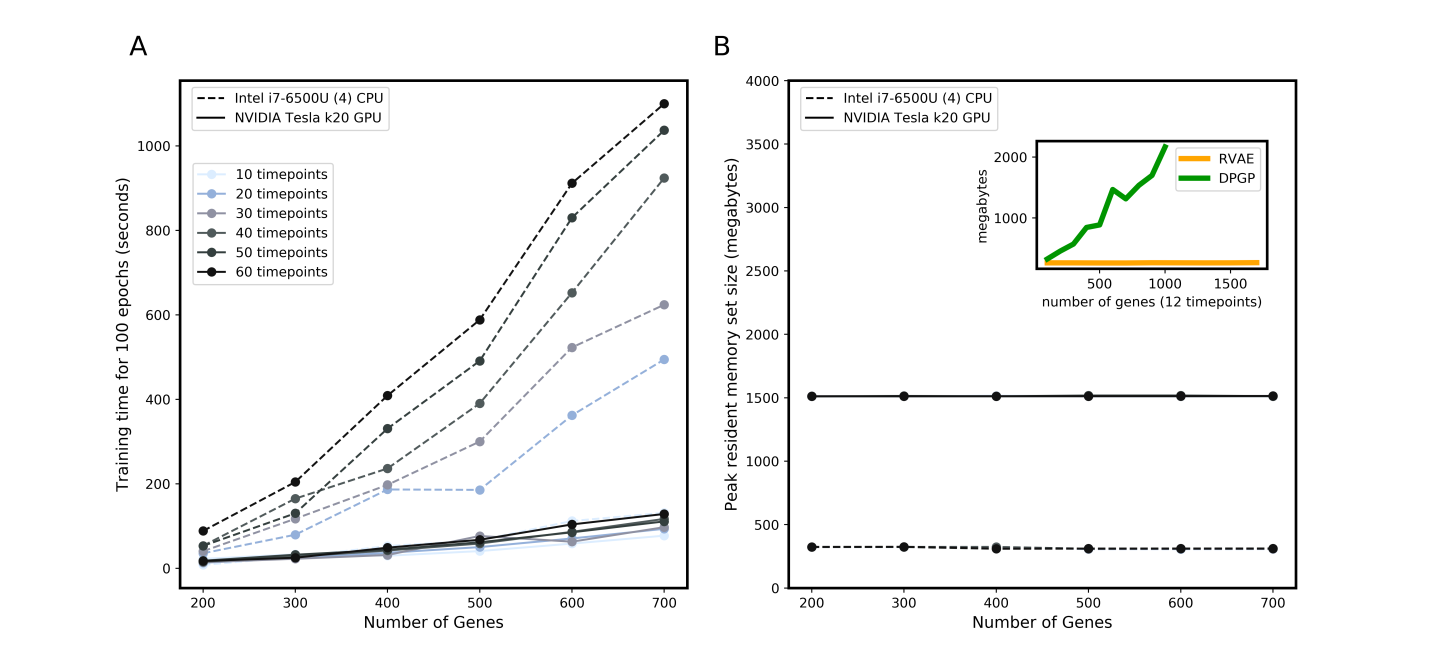
\includegraphics[width=0.8\paperwidth]{figures/fig7.png}}
 % archetecture.png: 1149x508 px, 72dpi, 40.53x17.92 cm, bb=0 0 1149 508
        \caption[Computational cost of training RVAgene]{\textbf{Training RVAgene is reasonably scalable on CPU and even more so using hardware acceleration through GPU.} ({\bf A}) Time cost of training RVAgene for 100 epochs for datasets with varying number of genes and time points on CPU and GPU. ({\bf B}) Maximum memory utilized during training of the model on CPU an GPU for the cases in (A), inset plot: comparison of max memory used compared to DPGP for varying number of genes.}
  \label{fig:fig7}
\end{figure}
\end{center}


\subsection{Assessment of the computational efficiency of RVAgene}

We assessed the computational efficiency of RVAgene for various settings and hardware. For the majority of the models trained, 100-200 epochs was sufficient for the loss function $\cL$ to converge. For tests performed here, we recorded the RVAgene runtime for 100 epochs of training using models that varied in their number of genes and time points. In each case we used a latent space of dimension two, a hidden size of 10, and a training batch size of 10. We ran the model on an intel i7 CPU with four cores and a Tesla K20 GPU. Runtimes were recorded on linux via the inbuilt time script (\texttt{/usr/bin/time --verbose}). As the number of time points and genes grew large (up to 60 time points and 700 genes), total runtimes on CPU were on the order of $10^3$ seconds ($<$ 20 minutes) (\hyperref[fig:fig7]{Fig. 6A}). On GPU, total runtimes were decreased to around $100$ seconds ($< 3$ minutes). Thus, RVAgene is readily scalable to tens of thousands of genes and hundreds of time points for training times of up to a few days on CPU or hours on GPU. For comparison, as described in \citet{McDowell2018}, the approximation-free time complexity of each iteration of learning for DPGP is $\cO(GT^3)$, due to the $G$ matrix inversions, each of size $T \times T$, for a dataset with $G$ genes and $T$ timepoints. The complexity for each epoch of training of RVAgene is $\cO(GT)$.
%The cubic complexity of the hierarchical Gaussian Process learning in DPGP quickly increases training time and does not allow scalability over timepoints without some form of approximation.
\par 
In terms of peak memory usage, since RVAgene is a neural network trained using backpropagation  \citep{rumelhart1986learning}, maximum memory used during training is of the same size as the network itself, which is constant given that the model parameters are fixed  (\hyperref[fig:fig7]{fig. 6B}). This is in contrast to Gaussian Processes (such as DPGP), which initially assign each gene to its own cluster, thus must store $G$ matrices of size $T\times T $, for $G$ genes and $T$ timepoints per gene. This leads to quickly increasing runtime peak resident set sizes for DPGP compared to RVAgene (\hyperref[fig:fig7]{fig. 6B} Inset). The memory used by DPGP grows with the number of time points as $\cO(GT^2)$). Thus, DPGP will not run with large numbers of genes and time points. %, and RVAgene has greater potential for the discovery of nuanced dynamical features in the data.
A note on this comparison: it is not direct, in the sense that DPGP performs clustering and RVAgene does not, in addition to other important differences between the goals of the methods. 
%However, we must add that direct comparisons must be made cautiously, given the differences between the two methods. 
%DPGP performs independent gene clustering; RVAgene does not (clustering can be performed downstream on the latent space).
Nonetheless, the size and scope of current biological datasets -- particularly at single-cell resolution -- in many cases preclude the use of DPGP without large reductions of the input data size. As we have shown, a feasible and efficient alternative in such cases is to run RVAgene, and then to perform clustering or other classification analyses post hoc on the latent space of the model. 


%what does it do?
%- visualization/classification (encoder) and prediction/generation (decoder)
%
%Plan
%- overview of main findings - ability to classify, predict, and generate 
%- current uses - tuning hyperparameters (DPGP) 
%- current uses - interpretability (cf. other VAEs)
%- future uses - interpretability - using LDVAE
%- future uses - (GRNs)
%- future work: time interval 
%- future work: discret time 
%- future work: different priors (cite SOUP)
%- conclusion


\section{Discussion}
{We have presented RVAgene, a recurrent variational autoencoder for generative modeling of gene expression time series data.
Through its encoder network, RVAgene provides means to visualize and classify gene expression dynamic profiles, which can lead to the discovery of biological processes.
Through its decoder network, RVAgene provides means to generate new gene expression dynamic profiles of either the full data or (in the case of single-cell studies) the pseudotime-smoothed data by sampling points from the latent space. In doing so, RVAgene can accurately reconstruct gene dynamics in complex biological data. As a by-product, on single-cell datasets the model directly produces smoothed outputs, useful for denoising gene expression time series data. RVAgene is efficient on temporally-rich whole genome datasets, in comparison to current existing methods. }
\par
RVAgene can be used to discover structure in the data, such as gene profile clusters. Popular
methods for clustering gene profiles such as Bayesian hierarchical clustering
\citep{cooke2011bayesian} or DPGP \citep{McDowell2018} detect the number of clusters in the data by
fitting a hyperparameter $\alpha$, the concentration parameter of the governing Dirichlet process
\citep{ferguson1973bayesian}. Although unsupervised, inevitably, the choice of $\alpha$ affects the
number of clusters output. Visualizing the data first with RVAgene can give an idea whether the data
favor clustering or a continuous representation. Thus analysis in RVAgene can guide the setting of
the hyperparameter $\alpha$ in DPGP and similar methods. In the case of ESC differentiation, DPGP
predicts 12 clusters (\hyperref[fig:figS3]{ Fig. S18}), yet most have very few members and many share
similar patterns. The RVAgene latent space for this dataset finds two major divisions in the data,
and orders the largest DPGP clusters along a spectrum (\hyperref[fig:fig3]{fig. 6.2D}), suggesting that DPGP might be overfitting the data. Indeed, the two methods can be used complementarily: RVAgene for high-level structure discovery and DPGP for clustering.
{In cases where learning a detailed noise model (at single time point resolution) is important to the user, DPGP or other Gaussian Process models are preferable over RVAgene.}
However, DPGP does not scale well with large datasets and thus cannot always be used
(\hyperref[fig:fig7]{fig. 6.6}).
\par 
The latent space of an RVAgene model encodes useful information about biological features, and in that sense provides biologically interpretable representations of the data. However, the representation is not interpretable in the sense that the components of the latent space do not have a physical meaning nor are they necessarily independent. Recent methods have tackled this issue of interpretability, by either modifying the loss function to make components independent \citep{higgins2016beta} or substituting linear functions in parts of the VAE \citep{svensson2020interpretable, ainsworth2018oi}. These methods have clear advantages regarding the analysis and interpretation of features in the latent space. In future work, decoding an RVAgene model with a linear function \citep{svensson2020interpretable} could facilitate additional discovery and improve our ability to gain insight into dynamic biological processes through the analysis of the latent space.
\par 
Dynamic changes in gene expression underlie essential cell processes. As such, modeling gene expression changes can also facilitate downstream analysis tasks, including gene regulatory network (GRN) inference. Inferring gene regulatory networks from single-cell data is challenging \citep{chen18_evaluating}, particularly due to cell-cell heterogeneity and high levels of noise. Several recent approaches to GRN inference make use of temporal profiles \citep{deshpande19_network, kim20_tenet}  
or differential equations \citep{ma20_inference, aubin-frankowski20_gene, matsumoto17_scode}. RVAgene could supplement such methods either by providing denoised input data, or by completely replacing the temporal ordering/differential equation-based components of these methods (which can be notoriously difficult to parameterize) with data produced from a RVAgene generative model of the gene expression dynamics.
\par 
RVAgene is currently agnostic of irregular time intervals between consecutive points in a time series,  i.e. it standardizes the time interval. This is not usually a concern for single-cell data, since with pseudotime information we can choose appropriate time intervals. However, in other cases, such as in response to kidney injury \citep{liu2017molecular}, standardizing time intervals distorts the dynamic profiles. Since RVAgene seeks to describe broad temporal patterns, we do not see this as a critical issue, though it would be desirable to generalize the model. A simple way to model irregularly spaced time points would be to augment the data through interpolation, though this is difficult without making strong assumptions about the (generally unknown) noise model. Gaussian process models \citep{McDowell2018, hensman2013hierarchical} can take irregular data as input, although (as noted above) are not efficient enough to run on large datasets. An alternative approach would be to modify the recurrent network architecture to take time points explicitly as input values, this would enable modeling of irregular or asynchronous data \citep{wu2018modeling}.
%\tcr{ https://link.springer.com/article/10.1186/1471-2105-14-252}
\par
RVAgene models in discrete time steps. There is no simple modification to the recurrent network structure that allows for prediction on continuously valued time. However, a recent development: neural ordinary differential equations (ODEs) \citep{chen2018neural}, enables modeling of time series data with continuous timepoints. \citet{chen2018neural} describe a generative latent ODE architecture similar to that of RVAgene, except that in their case the recurrent decoder network is replaced by a neural ODE decoder network. \citet{chen2018neural} demonstrate accurate results using synthetic data, however when we applied the method to the ESC single-cell differentiation dataset \citep{Klein2015}, the neural ODE network was found to converge very slowly and was overall underfit (\hyperref[fig:figS9]{Fig. S24}). The latent ODE method used by \citet{chen2018neural} does not address the challenge of modeling asynchronous/irregularly spaced data, but this has been more recently addressed \citep{rubanova2019latent}. These new models may well lead to future improvements in network architectures, although it seems that computational progress is needed before they can be successfully applied to complex biological systems.
%We will keenly follow developments in the field. 
\par 
In the current work, the prior on latent space used throughout was a unit spherical Normal, appropriate for exploratory data analysis where we have no further knowledge about structure in the latent space.
% ($\cN(\mathbf{0},\mathbf{I})$). 
However, given more information, e.g. that the data contains $k$ clusters, a different prior on the latent space might be more appropriate. A multi-modal prior -- such as a Gaussian Mixture Model (GMM) prior -- would permit structured (multi-modal) representations. However, the KL-divergence for an arbitrary GMM is not tractable; approximation  \citep{hershey2007approximating} or numerical computation would be necessary. Moreover, there is a greater problem: mixture models contain discrete parameters and VAE models are ill-suited for the optimization of discrete parameters \citep{dilokthanakul2016deep}, thus directly replacing the Normal prior of a VAE with a GMM is not feasible. A workaround to this problem is presented in \citep{dilokthanakul2016deep}, however implementing this for a recurrent model architecture remains an open problem. 
%A  k-modal prior would increase the probability of a latent space representation containing $\geq k$ clusters, i.e. increasing the structure of the space. 
%cite SOUP
\par 
The points raised above offer much scope for future work. These include the design of new latent space models with informative priors, modeling irregular time series data, and modeling in continuous time. Developments in some of these areas \citep{chen2018neural}, while promising, tend to rely on training data with relatively low levels of noise: far from the reality of most biological data. Thus it seems highly likely to be beneficial for both machine learning and biology to develop new neural network architectures in light of biological data. 











\section*{Acknowledgements}
We thank A.P. McMahon for valuable discussions and comments on the manuscript.
R.M. gratefully acknowledges support from a USC Viterbi Fellowship.

\section*{Data Availability}
The synthetic data used for evaluation of RVAgene are available at:
\url{https://github.com/maclean-lab/RVAgene}. Additional data used in the manuscript are available from the Gene Expression Omnibus: ESC differentiation (GEO accession GSE65525) and kidney injury (GEO accession GSE98622).

\section*{Software Availability}
RVAgene is available in Python released under an MIT license:  \url{https://github.com/maclean-lab/RVAgene}.


%%%%%%%%%%%%%%%%%%%%%%%%%%%%%%%%%%%%%%%%%%%%%%%%%%%%%%%%%%%%%%%%%%%%%%%%%%%%%%%%%%%%%%%%%%%%%%%%%%%%%%%%%%%%%%%%%%%%%%%%%%%%%%%%%%
%%%%%%%%%%%%%%%%%%%%%%%%%%%%%%%%%%%%%%%%%%%%%%%%%%%%%%%%%%%%%%%%%%%%%%%%%%%%%%%%%%%%%%%%%%%%%%%%%%%%%%%%%%%%%%%%%%%%%%%%%%%%%%%%%
\chapter{Conclusion and future work}
%\Chapter[Conclusion]{Conclusion}

I joined the QCB department at USC as a PhD student in August 2019. The rigorous curriculum of the CBB PhD program helped me shape my scientific vision and research skills. Soon, the COVID19 pandemic changed everything about our life and uncertainty covered the world. Thankfully, due to wise and loving care of the department, my adviser Prof. Remo Rohs and other members of the QCB department, I was able to continue my work through the difficult times. Prof. Adam MacLean orked hard to help me finish the RVAgene project and get it published \citep{Mitra2021}. The pandemic affected scientific travel oppportunities severely, during those intial years of my PhD. However, later on I was fortunate to be able to travel to numerous high quality conferences and present my work there. I am thankful to my advisor Prof. Remo Rohs for providing me with these opportunities. In fact, meeting Nobel laureate Prof. Ada Yonath (for solving the structure of ribosome \citep{schluenzen2000structure, harms2001high}) has been one of the most memorable experience of my life. I am also thankful to prof. Yonath for supporting us on the RNAscape project. 


Overall, it has been a fascinating experience to work in the intersection of artificial intelligence and structural biology during these past years. In 2021, we witnessed a more than half a century old problem, protein folding, being almost solved by AlphaFold2 \citep{Jumper2021}, as I was working on my project of modeling protein-DNA binding specificity based on structures. Efforts were immediately underway, to attempt to predict structures of higher order complexes of biomolecules \citep{evans2021protein,baek2024na}, and recently took a big step forward through AlphaFold3 \citep{Abramson2024}. However, these complex structure prediction methods, thus far, are not yet able to model binding specificity. This puts our model, DeepPBS \citep{Mitra2024}, which can look at a predicted or designed complex, and pedict binding specificity in a uniquely synergistic position. In my view, combination of structure prediction and specificity prediction methods is the future of predicting/desgining biologically meaningful complexes. In fact, a fresh direction of thinking about this problem is joint modeling of structure and specificity. However, this is still quite ambitious as data sparsity poses a big challenge, especially for complexes involving nucleic acids. 

Alongside my work on protein-DNA, concurrent events, and my advisor's encouragement inspired me to explore the field of RNA biology, which led to the projects, RNAscape and RNAproDB. As of now, the field of RNA structures is also being shaped by artificial intelligence methods \citep{he2024ribonanza}. However, an AlphaFold level breakthrough is still out of reach \citep{schneider2023will}. Recent works have shown progress in protein structure targeted RNA structure design \citep{nori2024rnaflow} and prediction of protein-RNA binding energy \citep{han2024copra}. Although promising, a lot of it is still quite preliminary and/or lacks biological validation. A DeepPBS like model for RNA binding specifcity prediction is also non-existent (although there has been some progress \citep{Lam2019}). It has also been known for a while that solvent molecules have an effect on protein-nucleic acid recognition \citep{Otwinowski1988}. However, the extent of this phenomenon has not been quantified.

Structure, function and localization of non-coding RNA is also something that remains to be studied and modelled. 70-90\% mammalian genome get transcribed into RNA, but only 1\% of it get translated. Rest are known as ncRNA (non coding RNA). lncRNAs are defined by their size range of 200 bases to 10kilobases. For a long time lncRNAs were regarded as only transcriptional noise. But, recently, it has been shown that they perform important important regulatory functions. Variations in lncRNA expression has been shown to be significantly correlated with certain disease traits \citep{wapinski2011long} and they are tissue-specific \citep{seifuddin2020lncrnakb}. LncRNA expression actually better explains certain cancer
classification data compared to mRNA expression \citep{al2019long}. Recent work on population-scale tissue transcriptomics \citep{de2021population} discovers high tissue specific regulation of lncRNA. They also identify 800 lncRNA-trait relationships which are not explained by protein coding genes. Hence, there is a growing interest in developing computational methods addressing various kinds of biological problems in lncRNAome. \citep{alam2020deep} discusses Deep Learning methods recently being developed for
such tasks. Some of these works include, lncRNA-protein interaction prediction
\citep{pan2016ipminer, zhao2018bipartite, yi2018deep, zhan2019bgfe, peng2019rpiter}, lncRNA  identification \citep{baek2018lncrnanet,yang2018lncadeep, tripathi2016deeplnc},
learning regulatory information \citep{alam2019deepcnpp, alam2019deepel}, predicting subcellular localization of lncRNAs \citep{gudenas2018prediction},    lncRNA-miRNA interaction prediction \citep{huang2019predicting}, lncRNA-disease association prediction \citep{hu2019deep, xuan2019dual, al2019long, xuan2019graph} etc. All these tools might improve in future through incorporation of structural and specificity information, as structure and specifcity prediction methods evolve over time.

With the improvements in structure prediction and design, there is an increasing need of high quality analysis tools for the biologists to be able to study, visualize and explore these structures. In later part of my PhD, we built an updated DNAproDB, RNAscape \citep{Mitra2024rnascape} and RNAproDB to address this need. These tools are 
designed to 

Data driven modeling, especially probabilistic machine learning, has been the main theme of my
research. I am extremely grateful for being able to work with so many great minds here at USC and I
hope I can make more meaningful contributions to the collective gathering of human knowledge in
future. Thus I conclude my dissertation proposal.

%%%%%%%%%%%%%%%%%%%%%%%%%%%%%%%%%%%%%%%%%%%%%%%%%%%%%%%%%%%%%%%%%%%%%%%%%%%%%%%%%%%%%%%%%%%%%%%%%%%%%%%%%%
% Conclusion and ongoing work
%\include{main/Conclusion}

% Using single-space for reference list.
\begin{singlespace}
% Bibliography
%\phantomsection
%\addcontentsline{toc}{chapter}{References}%
%\markboth{References}{References}%
% If you use BibLaTeX
\printbibliography%[title=References]
% If you use BibTeX
%\bibliography{library}
%\bibliographystyle{agsm}
\end{singlespace}

%\subsection*{Supplementary figures}
\label{supp}

\renewcommand{\thefigure}{S\arabic{figure}}
\setcounter{figure}{0}
%% DeepPBS SUPP FIGURES
\begin{center}
\begin{figure}[H]
  \includegraphics[width=\linewidth]{./pdnafigs/figS1.png}
 % archetecture.png: 1149x508 px, 72dpi, 40.53x17.92 cm, bb=0 0 1149 508
    \caption[Dataset details.]{\textbf{Dataset details.} ({\bf a}) Schematic representation of process for combining data sources. ({\bf b}) Distribution of source experiments and species in constructed cross-validation set. ({\bf c}) Example illustration demonstrating differences in binding specificity data for the same protein (human estrogen receptor 1) from different experiments and databases. Mean absolute error (MAE) over columns among three cases.}
  \label{fig:pdnaS1}
\end{figure}
\end{center}

\begin{center}
\begin{figure}[H]
  \includegraphics[width=\linewidth]{./pdnafigs/figS2.png}
 % archetecture.png: 1149x508 px, 72dpi, 40.53x17.92 cm, bb=0 0 1149 508
    \caption[Data Representation.]{\textbf{Data Representation.} ({\bf a}) Coarse-grain symmetrization schema at DNA base-pair level. ({\bf b}) Example illustration showing how the computed sym-helix compares with the original structure. Each sym-helix point is shown as a sphere (1.5 \AA radius) for visibility. ({\bf c})Symmetrized base-pair representation on one C-G base pair (four major groove points, three minor groove points, and two points each for sugar and phosphate moieties). ({\bf d}) Example computed shape features overlayed on sym-helix as base pair-level features. ({\bf e}) Standard vectors computed on sym-helix, used by the network to correlate orientation information with ({\bf f}) interaction vectors on protein atom-graph, based on average direction of covalent bonds for each heavy atom.}
  \label{fig:pdnaS2}
\end{figure}
\end{center}

\begin{center}
\begin{figure}[H]
  \includegraphics[width=\linewidth]{./pdnafigs/figS3.png}
 % archetecture.png: 1149x508 px, 72dpi, 40.53x17.92 cm, bb=0 0 1149 508
    \caption[DeepPBS architecture.]{\textbf{DeepPBS architecture.} The DeepPBS architecture can be compartmentalized into three modules: ProteinEncoder,
which encodes the protein neighborhood through spatial graph convolutions; BiNet, which consists of a network of
bipartite geometric convolutions from the protein graph ($G^p =
(V^p, X^p, E^p, N^p))$ to sym-helix points (DNA) ($G^d = (v^d, X^d, N^d))$; and CNN-Predictor, which flattens the aggregated sym-helix features into a 1D representation, adds shape features ($X^s$),
and applies 1D convolutional layers followed by fully connected prediction layers. The final logits are converted into probability using a SoftMax activation with a learned temperature parameter. $E_{r=x}$ represents edges determined by vertices/points within a specified radius of length $x$. Each sym-helix point is shown as a sphere (1.5 \AA radius) for visibility.}
  \label{fig:pdnaS3}
\end{figure}
\end{center}

\begin{center}
\begin{figure}[H]
  \includegraphics[width=\linewidth]{./pdnafigs/figS4.png}
 % archetecture.png: 1149x508 px, 72dpi, 40.53x17.92 cm, bb=0 0 1149 508
    \caption[Schematic representation of bipartite edge-perturbation process.]{\textbf{Schematic representation of bipartite edge-perturbation process.} Blue circles denote protein heavy atoms.
Green circles represent sym-helix points. In one forward pass, the output is calculated with all edges present. In
another pass, edges corresponding to one protein heavy atom are excluded from the message-passing scheme,
resulting in an alternate output. The difference between the two outputs can be quantified using the mean absolute
difference measure and normalized as needed for interpretation purposes.}
  \label{fig:pdnaS4}
\end{figure}
\end{center}

\begin{center}
\begin{figure}[H]
  \includegraphics[width=\linewidth]{./pdnafigs/figS5.png}
 % archetecture.png: 1149x508 px, 72dpi, 40.53x17.92 cm, bb=0 0 1149 508
    \caption[Cross-validation performance of DeepPBS for predicting binding specificity across protein families on
experimentally determined structures.]{\textbf{Cross-validation performance of DeepPBS for predicting binding specificity across protein families on experimentally determined structures.} Caption on next page.}
  \label{fig:pdnaS5}
\end{figure}
\addtocounter{figure}{-1}
\begin{figure} [H]
  \caption[Cross-validation performance of DeepPBS for predicting binding specificity across protein families on experimentally determined structures.]{\textbf{Cross-validation performance of DeepPBS for predicting binding specificity across protein families on experimentally determined structures.}({\bf a}) Cross-validation performance of individual trained models for the DeepPBS model and its variations (biological assemblies corresponding to $n$= 523 protein chains (for each box plot)) ({\bf b}) Abundance of various protein families (PFAM annotations) in cross-validation dataset (counts$>$8). ({\bf c}) Cross-validation performance of DeepPBS, along with ‘groove readout’ and ‘shape readout’ variations, across protein families (counts $>$ 8). (Biological assemblies corresponding to $n$ protein chains (for each family), where $n$ is as described in ({\bf b}), total unique $n$= 523) ({\bf d}) Example DeepPBS ensemble prediction on NF-$\kappa$B biological assembly (sampled in benchmark set) containing non-optimal DNA sequence. DeepPBS ensemble prediction on NF-$\kappa$B biological assembly for human (NFKB2, UniProt ID Q00653) is shown in the benchmark dataset. The colored heatmaps (top and bottom) encode probabilities of base identity. The back and white heatmap (center) represents the co-crystal structure. Although the co-crystal structure derived DNA sequence is not of the highest affinity (judging by experimental data from HOCOMOCO), our prediction can circumvent this issue and predict binding specificity levels that are much closer to those observed experimentally. For box plots in ({\bf a}) and ({\bf c}), lower limit represents lower quartile, middle line represents median, and upper limit represents upper quartile. Whiskers do not include outliers.}
\end{figure}
\end{center}

\begin{center}
\begin{figure}[H]
  \includegraphics[width=\linewidth]{./pdnafigs/figS6.png}
 % archetecture.png: 1149x508 px, 72dpi, 40.53x17.92 cm, bb=0 0 1149 508
    \caption[Application of DeepPBS to MD simulation of AlphaFold2- and PDB (2R5Z)-based modeled complex of Exd-
Scr system. ]{\textbf{Application of DeepPBS to MD simulation of AlphaFold2- and PDB (2R5Z)-based modeled complex of Exd-Scr system.} ({\bf a}) Initial structure of simulation. Locations of residues of interest are marked. ({\bf b}) Residue-level RI score over time (averaged per 5 ns window) for residues involved in Exd-DNA flank ineraction. ({\bf c}) Snapshot of interactions by Exd Arg2, Arg3, and Arg5 at 50 ns, 200 ns, and 280 ns, respectively. ({\bf d}) Residue-level RI score over time (averaged 5 ns window) for residues involved in Scr-DNA minor groove interaction. ({\bf e}) Snapshot of interactions by Scr Arg5 and His-12 at 70 ns and 250 ns, respectively. ({\bf f}) Residue-level RI score over time (averaged per 5 ns window) for residues involved in Scr-DNA major groove interaction. ({\bf g}) Snapshot of interactions by Exd Arg58, Lys6, and Ile57 at 70 ns and 250 ns.}
  \label{fig:pdnaS6}
\end{figure}
\end{center}

\begin{center}
\begin{figure}[H]
  \includegraphics[width=\linewidth]{./pdnafigs/figS7.png}
 % archetecture.png: 1149x508 px, 72dpi, 40.53x17.92 cm, bb=0 0 1149 508
    \caption[Example DeepPBS ensemble predictions on structures of specific DNA binders.]{\textbf{Example DeepPBS ensemble predictions on structures of specific DNA binders.} Specificity data were
unavailable on JASPAR/HOCOMOCO.  ({\bf a}) Monomeric orphan nuclear receptor NGFI-B, ({\bf b}) replication termination protein in bacteria, ({\bf c}) proto-oncogene product c-Rel, ({\bf d}) Tc3 transposase bound to transposon DNA, ({\bf e}) Fitab protein from \textit{Neisseria gonorrhoeae}, ({\bf f}) Epstein-Barr virus ZEBRA protein, ({\bf g}) Smad5-MH1 protein/ palindromic SBE DNA complex, and ({\bf h}) DUF1778 domain-containing kacTA protein.}
  \label{fig:pdnaS7}
\end{figure}
\end{center}

\begin{center}
\begin{figure}[H]
  \includegraphics[width=\linewidth]{./pdnafigs/figS8.png}
 % archetecture.png: 1149x508 px, 72dpi, 40.53x17.92 cm, bb=0 0 1149 508
    \caption[Example DeepPBS ensemble predictions on structures of non-specific DNA binders.]{\textbf{Example DeepPBS ensemble predictions on structures of non-specific DNA binders.} ({\bf a}) Sso7D-DNA complex,
({\bf b}) DNA polymerase I Klenow fragment,  ({\bf c}) HIV-1 reverse transcriptase with pre-translocation and post-translocation AZTMP-terminated DNA,  ({\bf d}) DNA polymerase IV,  ({\bf e}) Moloney murine leukemia virus reverse transcriptase,  ({\bf f}) DNA repair enzyme formamidopyrimidine-DNA glycosylase (Fpg),  ({\bf g}) DNA polymerases in complex with proliferative cell nuclear antigen (PCNA), and  ({\bf h}) DNA damage sensing enzyme \textit{Methanococcus jannaschii} Mre11 (MjMre11).}
  \label{fig:pdnaS8}
\end{figure}
\end{center}

\begin{center}
\begin{figure}[H]
  \includegraphics[width=\linewidth]{./pdnafigs/figS9.png}
 % archetecture.png: 1149x508 px, 72dpi, 40.53x17.92 cm, bb=0 0 1149 508
    \caption[Application of DeepPBS on modeled structures.]{\textbf{Application of DeepPBS on modeled structures.} ({\bf a}) Performance of DeepPBS (best 6-mer overlap) improves as
the feedback loop progresses (corresponding to Fig. 3f) in conjunction with improvement in RFNA complex design. ($n$ = 236 predicted assemblies) ({\bf b}) Example application of DeepPBS on mouse CREB1 dimer bound to DNA modeled
by MELD-DNA (as provided by their authors). ({\bf c}) Calculated MM-PBSA (Supplementary Section 7) vacuum energy
distribution for stable RFNA predictions ($<$0 kJ/mol) and corresponding counts over rounds 1–7 (for $n$ predicted
assemblies for each boxplot, where $n$ is same as stable structure count (corresponding bar plot)). For box plots in ({\bf a})
and ({\bf c}), lower limit represents lower quartile, middle point/line represents median, and upper limit represents upper
quartile.}
  \label{fig:pdnaS9}
\end{figure}
\end{center}

\begin{center}
\begin{figure}[H]
  \includegraphics[width=\linewidth]{./pdnafigs/figS10.png}
 % archetecture.png: 1149x508 px, 72dpi, 40.53x17.92 cm, bb=0 0 1149 508
    \caption[Behavior of metric for different target PWM and interpolated predictions.]{\textbf{Behavior of metric for different target PWM and interpolated predictions.} ({\bf a}) Demonstrations of how the MAE
metric behaves for various different target PWM columns and possible predictions (Fig. S10a). The predictions are of three forms, based on interpolated values of a variable $x \in [0,1]$ . Although not an exhaustive set, we hope it helps the reader put into context the behavior of this metric. ({\bf b}) DeepPBS
and DeepPBS with DNA SeqInfo performance on benchmark set in context of two naive models (uniform predictor
and co-crystal structure derived sequence predictor). Lines indicates linear regression fit. Light shaded regions
indicate corresponding 95$\%$ confidence interval computed via bootstrapping mean.}
  \label{fig:pdnaS10}
\end{figure}
\end{center}

\begin{center}
\begin{figure}[H]
  \includegraphics[width=\linewidth]{./pdnafigs/figS11.png}
 % archetecture.png: 1149x508 px, 72dpi, 40.53x17.92 cm, bb=0 0 1149 508
    \caption[MAE equivalent of benchmark performance vs alignment score plot.]{\textbf{MAE equivalent of benchmark performance vs alignment score plot}  showing the bias of the DeepPBS with DNA SeqInfo model compared to the DeepPBS model towards the alignment score of co-crystal DNA structure derived sequence and target PWM. Lines indicates linear regression fit. Light shaded regions indicate corresponding 95$\%$ confidence interval computed via bootstrapping mean.}
  \label{fig:pdnaS11}
\end{figure}
\end{center}

\begin{center}
\begin{figure}[H]
  \includegraphics[width=\linewidth]{./pdnafigs/figS12.png}
 % archetecture.png: 1149x508 px, 72dpi, 40.53x17.92 cm, bb=0 0 1149 508
    \caption[Deep DNAshape prediction of the minor groove width (MGW) profile]{\textbf{Deep DNAshape \citep{Li2023} prediction of the minor groove width (MGW) profile} for the sequence AAATTG (top DeepPBS
prediction for the designed model DBP35 and DBP5, positions 3–8) compared to the actual MGW of the DNA in
these designed complexes.}
  \label{fig:pdnaS12}
\end{figure}
\end{center}
%% RNASCAPE SUPP FIGURES
\begin{center}
\begin{figure}[H]
  \includegraphics[width=\linewidth]{./rnascapefigs/figureS1.png}
 % archetecture.png: 1149x508 px, 72dpi, 40.53x17.92 cm, bb=0 0 1149 508
    \caption[Tertiary structure aware mapping of the peptidyl transferase center (PTC) of the large ribosomal subunit of Deinococcus radiodurans (PDB ID: 1NKW), also known as proto-ribosome ]{\textbf{Tertiary structure aware mapping of the peptidyl transferase center (PTC) of the large ribosomal subunit of Deinococcus radiodurans (PDB ID: 1NKW), also known as proto-ribosome.} ({\bf A}) Principal axis view of the PTC \citep{Bose2022}. ({\bf B})  Rotated view (approximately 90° about horizontal axis). ({\bf C})  RNAscape visualization of the proto-ribosome in orientation along the principal axis view. ({\bf D})  RNAView \citep{Yang2003} visualization of the proto-ribosome in orientation along the principal axis view. Unlike RNAView, RNAscape captures the semi-symmetric nature of the structure.}
  \label{fig:rnascapeS1}
\end{figure}
\end{center}

\begin{center}
\begin{figure}[H]
  \includegraphics[width=\linewidth]{./rnascapefigs/figureS2.png}
 % archetecture.png: 1149x508 px, 72dpi, 40.53x17.92 cm, bb=0 0 1149 508
    \caption[RNAscape web interface for side-by-side comparison of two structures.]{\textbf{RNAscape web interface for side-by-side comparison of two structures.} ({\bf A}) 3D structure of PDB ID: 8UPT and ({\bf B}) 3D structure of PDB ID: 8UPY. ({\bf C}) After running RNAscape on one structure (in this example, PDB ID: 8UPT \citep{Krahn2024}, a user can upload a second plot for side-by-side comparison (in this example, PDB ID: 8UPY \citep{Krahn2024}. Both plots have separate transformation controls which can be used to orient and compare them.}
  \label{fig:rnascapeS2}
\end{figure}
\end{center}

\begin{center}
\begin{figure}[H]
  \includegraphics[width=\linewidth]{./rnascapefigs/figureS3.png}
 % archetecture.png: 1149x508 px, 72dpi, 40.53x17.92 cm, bb=0 0 1149 508
    \caption[Visualization of a riboswitch by various methods.]{\textbf{Visualization of a riboswitch by various methods.} ({\bf A}) Riboswitch from Escherichia coli (PDB ID: 1Y26) ({\bf B}) RNAscape visualization. ({\bf C}) RNAView \citep{Yang2003} visualization (rotated to align with the 3D structure.). ({\bf D}) RNAglib \citep{Mallet2022} visualization. ({\bf E}) Seondary structure visualization based on the structure by Forna \citep{Kerpedjiev2015}.}
  \label{fig:rnascapeS3}
\end{figure}
\end{center}
\begin{center}
\begin{figure}[H]
  \includegraphics[width=\linewidth]{./figures/noisy_sim.png}
 % archetecture.png: 1149x508 px, 72dpi, 40.53x17.92 cm, bb=0 0 1149 508
    \caption[Demonstration of RVAgene working principle on simulated data with high noise.]{\textbf{Demonstration of RVAgene working principle on simulated data with high noise.} Gaussian noise drawn from $\cN(0,0.7)$ was added to the simulated data to produce a dataset with heavy noise. RVAgene learns the latent space shown in ({\bf A}). ({\bf B}) shows 6 clusters learned by k-means on the learned latent space. ({\bf C}) shows original training data and model generated data from random points in the latent space sampled from $\cN(\mu,0.4\bI)$ around each cluster mean $\mu$ for each of the 6 clusters detected by k-means.}
  \label{fig:figS1}
\end{figure}
\end{center}
\newpage

\begin{center}
\begin{figure}[H]
  \includegraphics[width=\linewidth]{./figures/sl_ESC_r.png}
 % archetecture.png: 1149x508 px, 72dpi, 40.53x17.92 cm, bb=0 0 1149 508
    \caption[Characterization of gene dynamics by linear fit using Pearson correlation coefficient for 5 sample genes in the ESC differentiation dataset]{Characterization of gene dynamics by linear fit using Pearson correlation coefficient for 5 sample genes in the ESC differentiation dataset  \citep{Klein2015}. Blue lines represents original data and orange lines represents linear fits. The Pearson correlation coefficient $r$ is given for each plot.}
  \label{fig:figS2}
\end{figure}
\end{center}
\newpage

\begin{center}
\centering
\begin{figure}[H]
  \includegraphics[width=\linewidth,height=0.4\textheight]{figures/fig4.png}
 % archetecture.png: 1149x508 px, 72dpi, 40.53x17.92 cm, bb=0 0 1149 508
    \caption[Clusters detected by the unsupervised clustering algorithm DPGP for ESC differentiation.]{\textbf{Clusters detected by the unsupervised clustering algorithm DPGP for ESC differentiation.} Clusters detected by DPGP in the ESC differentiation dataset  \citep{Klein2015} with default hyperparameters showing cluster means (black), mean $\pm$ 2 s.d. in (blue) and cluster members (red). }
   \label{fig:figS3}
\end{figure}
\end{center}
\newpage
\begin{center}
\begin{figure}
  \includegraphics[width=\linewidth]{./figures/supp_varying_test_set_sizes.png}
 % archetecture.png: 1149x508 px, 72dpi, 40.53x17.92 cm, bb=0 0 1149 508
    \caption[Accuracy of RVAgene reconstructions for different train/test group sizes.]{{\bf Accuracy of RVAgene reconstructions for different train/test group sizes.} Distributions of reconstruction errors on randomly sampled sets of test genes, where the full data were split into test groups of: 200 genes (train on 72\%), 300 genes (train on 59\%), 400 genes (train on 45\%), 500 genes (train on 31\%), and 600 genes (train on 18\%). Cumulative fractional distribution of reconstruction errors (cumulative count/test set size) for all groups.}
  \label{fig:figS4}
\end{figure}
\end{center}
\newpage

\begin{center}
\begin{figure}[H]
  \includegraphics[width = \linewidth]{figures/fig8.png}
 % archetecture.png: 1149x508 px, 72dpi, 40.53x17.92 cm, bb=0 0 1149 508
    \caption[Modeling response to kidney injury and analysis of linear fits.]{\textbf{Modeling response to kidney injury and analysis of linear fits.}
    ({\bf A}) Pearson correlation coefficients between gene expression and time for each differentially expressed gene in the kidney injury dataset for each of the 3 replicates \citep{liu2017molecular}. ({\bf B}) RVAgene latent space representation of fitted model for each replicate; color represents positive or negative correlation coefficients. ({\bf C}) RVAgene latent space representation learnt for the same three replicates as in (B), but where every input gene was normalized  so that its expression sums to 1.}
  \label{fig:figS5}
\end{figure}
\end{center}
\newpage

\begin{center}
\begin{figure}[H]
  \includegraphics[width=\linewidth]{./figures/sl_JCI_r.png}
 % archetecture.png: 1149x508 px, 72dpi, 40.53x17.92 cm, bb=0 0 1149 508
    \caption[Comparison of linear and quadratic fits to describe gene dynamics in response to kidney injury.]{\textbf{Comparison of linear and quadratic fits to describe gene dynamics in response to kidney injury.}
    For each of the three replicates (R1-R3), five genes are shown, with experimental data (blue), linear fit (orange), and quadratic fit (green). 
    Pearson correlation coefficients, $r$, and quadratic coefficients, $a$ ($x = at^2 + bt + c$), are given for each plot.}
  \label{fig:figS6}
\end{figure}
\end{center}
\newpage

\begin{center}
\begin{figure}[H]
  \includegraphics[width=\linewidth]{./figures/supp_go.png}
 % archetecture.png: 1149x508 px, 72dpi, 40.53x17.92 cm, bb=0 0 1149 508
    \caption[Clustering on R1 and cluster specific GO enrichment analysis.]{\textbf{Clustering on R1 and cluster specific GO enrichment analysis.} We performed k-means clustering on latent space learned by RVAgene on R1 with $k=9$. We also show learned latent space on R2 and R3 annotated by the clustering done on R1. All clusters (except cluster 5) appears well preserved. We perform GO analysis for each cluster and select one significant GO term from each cluster (except cluster 5) and show how all genes in the dataset corresponding to each GO term appears on the latent space for all three replicates. }
  \label{fig:figS8}
\end{figure}
\end{center}
\newpage

\begin{center}
\begin{figure}[H]
  \includegraphics[width=\linewidth]{./figures/sdc_sl.png}
 % archetecture.png: 1149x508 px, 72dpi, 40.53x17.92 cm, bb=0 0 1149 508
    \caption[RVAgene latent space captures biological processes driving concordant gene expression changes (Sdc1).]{{\bf (A)} Latent space representations for replicates R1-R3 with local neighborhoods of Sdc1 marked (circles). ({\bf B}) Heatmap of expression changes over time course of injury for the Sdc1 neighborhood genes in the intersection of R1-R3; selected genes highlighted.  ({\bf C}) Histogram of -log10 p values of top GO terms for biological processes for gene set in (B).
    {\bf D}) Reconstructed vs true data plotted for each of the Lox genes identified in (B).}
  \label{fig:figS7}
\end{figure}
\end{center}

\begin{center}
\begin{figure}[H]
  \includegraphics[width=\linewidth]{./figures/latent_ode_val_underfit.png}
  % archetecture.png: 1149x508 px, 72dpi, 40.53x17.92 cm, bb=0 0 1149 508
    \caption[Examples of continuous time prediction of ESC differentiation.]{\textbf{Examples of continuous time prediction of ESC differentiation.} Reconstruction (up to $t=6.8$) and future prediction (for $t>6.8$) for 4 example genes by a  latent ODE \citep{chen2018neural} trained on ESC data \citep{Klein2015} for 1000000 iterations, showing a good fit for the initial timepoints, but underfitting for the later timepoints.}
  \label{fig:figS9}
\end{figure}
\end{center}

\begin{center}
    \begin{figure}[H]
    \makebox[\textwidth]{\includegraphics[width=0.7\textwidth]{./crffigs/lys.png}}
 % archetecture.png: 1149x508 px, 72dpi, 40.53x17.92 cm, bb=0 0 1149 508
        \caption[Interaction propensities of components of lysine amino acid towards various DNA moieties and functional groups]{\textbf{ Interaction propensities of components of lysine amino acid towards various DNA moieties and functional groups.} ({\bf a}) Interaction  propensity towards DNA bases  A,C,G,T, in addition to phosphate (P) and sugar (S) moieties, categorized by major groovre , minor groove and all (major,minor groove and DNA backbone) ({\bf b}) Interaction  propensity towards functional groups \citep{Chiu2023} A ((H-bond acceptor), D (H-bond donor), M (methyl),H (hydrogen)), in addition to phosphate (P) and sugar (S) moieties, categorized by major groovre , minor groove and all (major,minor groove and DNA backbone)}
  \label{fig:lys}
\end{figure}
\end{center}

\begin{center}
    \begin{figure}[H]
    \makebox[\textwidth]{\includegraphics[width=0.7\textwidth]{./crffigs/his.png}}
 % archetecture.png: 1149x508 px, 72dpi, 40.53x17.92 cm, bb=0 0 1149 508
        \caption[Interaction propensities of components of histidine amino acid towards various DNA moieties and functional groups]{\textbf{ Interaction propensities of components of histidine amino acid towards various DNA moieties and functional groups.} ({\bf a}) Interaction  propensity towards DNA bases  A,C,G,T, in addition to phosphate (P) and sugar (S) moieties, categorized by major groovre , minor groove and all (major,minor groove and DNA backbone) ({\bf b}) Interaction  propensity towards functional groups \citep{Chiu2023} A ((H-bond acceptor), D (H-bond donor), M (methyl),H (hydrogen)), in addition to phosphate (P) and sugar (S) moieties, categorized by major groovre , minor groove and all (major,minor groove and DNA backbone)}
  \label{fig:his}
\end{figure}
\end{center}

\begin{center}
    \begin{figure}[H]
    \makebox[\textwidth]{\includegraphics[width=0.7\textwidth]{./crffigs/asn.png}}
 % archetecture.png: 1149x508 px, 72dpi, 40.53x17.92 cm, bb=0 0 1149 508
        \caption[Interaction propensities of components of asparagine amino acid towards various DNA moieties and functional groups]{\textbf{ Interaction propensities of components of asparagine amino acid towards various DNA moieties and functional groups.} ({\bf a}) Interaction  propensity towards DNA bases  A,C,G,T, in addition to phosphate (P) and sugar (S) moieties, categorized by major groovre , minor groove and all (major,minor groove and DNA backbone) ({\bf b}) Interaction  propensity towards functional groups \citep{Chiu2023} A ((H-bond acceptor), D (H-bond donor), M (methyl),H (hydrogen)), in addition to phosphate (P) and sugar (S) moieties, categorized by major groovre , minor groove and all (major,minor groove and DNA backbone)}
  \label{fig:asn}
\end{figure}
\end{center}

\begin{center}
    \begin{figure}[H]
    \makebox[\textwidth]{\includegraphics[width=0.7\textwidth]{./crffigs/ser.png}}
 % archetecture.png: 1149x508 px, 72dpi, 40.53x17.92 cm, bb=0 0 1149 508
        \caption[Interaction propensities of components of serine amino acid towards various DNA moieties and functional groups]{\textbf{ Interaction propensities of components of serine amino acid towards various DNA moieties and functional groups.} ({\bf a}) Interaction  propensity towards DNA bases  A,C,G,T, in addition to phosphate (P) and sugar (S) moieties, categorized by major groovre , minor groove and all (major,minor groove and DNA backbone) ({\bf b}) Interaction  propensity towards functional groups \citep{Chiu2023} A ((H-bond acceptor), D (H-bond donor), M (methyl),H (hydrogen)), in addition to phosphate (P) and sugar (S) moieties, categorized by major groovre , minor groove and all (major,minor groove and DNA backbone)}
  \label{fig:ser}
\end{figure}
\end{center}

\begin{center}
    \begin{figure}[H]
    \makebox[\textwidth]{\includegraphics[width= 0.9\paperwidth]{./rnaprodbfigs/figS1.png}}
 % archetecture.png: 1149x508 px, 72dpi, 40.53x17.92 cm, bb=0 0 1149 508
        \caption[RNAproDB search page showing card view results for the keyword search ``tetrahymena"]{\textbf{ RNAproDB search page showing card view results for the keyword search ``tetrahymena".}}
  \label{fig:rnaprodbS1}
\end{figure}
\end{center}

\begin{center}
    \begin{figure}[H]
    \makebox[\textwidth]{\includegraphics[width= 0.9\paperwidth]{./rnaprodbfigs/figS2.png}}
 % archetecture.png: 1149x508 px, 72dpi, 40.53x17.92 cm, bb=0 0 1149 508
        \caption[RNAproDB output page for uploaded AlphaFold3 predicted structure (model 0) for PDB ID: 8AW3]{\textbf{ RNAproDB output page for uploaded AlphaFold3 predicted structure (model 0) for PDB ID: 8AW3.}}
  \label{fig:rnaprodbS2}
\end{figure}
\end{center}
\begin{center}
    \begin{figure}[H]
    \makebox[\textwidth]{\includegraphics[width= 0.9\paperwidth]{./rnaprodbfigs/figs3.png}}
 % archetecture.png: 1149x508 px, 72dpi, 40.53x17.92 cm, bb=0 0 1149 508
         \caption[Multiple mapping algorithms available in RNAproDB for protein-NA-hybrid complex (PDB ID: 4OO8)]{\textbf{Multiple mapping algorithms available in RNAproDB for protein-NA-hybrid complex (PDB ID: 4OO8).} ({\bf A}) Crystal structure of of Streptococcus pyogenes Cas9 in complex with guide RNA (red) and target DNA (blue) (PDB ID: 4OO8).  ({\bf B})  Mapping produced based on partial projection. ({\bf C}) Mapping produced based on RNAscape algorithm. ({\bf D}) Mapping produced by applying ViennaRNA secondary structure layout algorithm. Centroid distance cut off of $9 \AA$ was used for protein-NA interaction edges.}
  \label{fig:rnaprodbS3}
\end{figure}
\end{center}
\begin{center}
    \begin{figure}[H]
    \makebox[\textwidth]{\includegraphics[width= 0.9\paperwidth]{./pdnafigs/figS32.png}}
 % archetecture.png: 1149x508 px, 72dpi, 40.53x17.92 cm, bb=0 0 1149 508
         \caption[Step-by-step building of a symmetrized DNA base-pair.]{\textbf{\red{Step-by-step building of a symmetrized DNA base-pair.}}}
  \label{fig:pdnaS32}
\end{figure}
\end{center}

% Appendices
\phantomsection
\addcontentsline{toc}{chapter}{Appendices}%
\markboth{Appendices}{Appendices}%
\chapter*{Appendices}
\section*{Appendix A}
\addcontentsline{toc}{section}{Appendix A}%
\renewcommand\thesection{\Alph{section}}
\renewcommand*{\thesubsection}{\Alph{section}.\arabic{subsection}}
\begingroup
\numberwithin{equation}{section}
% Appendix source files
%\input{main/appendix_proof}

%SetFonts


%\date{}							% Activate to display a given date or no date

\section*{Detailed calculation of the CCRF layer update}
Starting from the mean field variational inference result in eq. \ref{mean_field_VI_result} we have, %\red{(Kr\"{a}henb\"{u}hl, 2012)} we have,
\label{crf_detailed}
\begin{equation}
Q_i (H_i) \simeq \frac{1}{Z} \exp \left ( - \alpha || H_i - B_i ||^2  - \beta \sum_{j \in \mathcal{N}(i)} g_{ij} \int_{-\infty}^{\infty} Q(H_j) ||H_i - H_j ||^2 d H_j\right )
\end{equation}

where $H_i, B_i, H_j \in \mathbb{R}^N$. Evaluating this component-wise and using the definition of the $\ell_2$ norm, we can write the energy $E(H_i)$ as

\begin{equation}
E(H_i) = \alpha \sum_n^N (H_{in} - B_{in})^2 + \beta \sum_{j \in \mathcal{N}(i)} g_{ij} \sum_n^N \int_{-\infty}^{\infty} \cdots \int_{-\infty}^{\infty} Q(H_j) (H_{in} - H_{jn})^2 d H_{j1}\cdots dH_{jN}
\end{equation}.

Focusing on the inner most summation of second term, since each component of $H_i$ and $H_j$ is
independent (by eq. 10 of \citet{gao2019conditional}), we can write $Q(H_j) = \Pi_{k=1}^N Q_{jk}(H_{jk})$ and assume that each $Q_{jk}$ is individually normalized. The summation then becomes

\begin{multline}
 \sum_n^N \int_{-\infty}^{\infty}  Q(H_j) (H_{in} - H_{jn})^2 d H_{j1}\cdots dH_{jN} \\
= \sum_n^N \int_{-\infty}^{\infty} (H_{in} - H_{jn})^2  \Pi_{k=1}^N Q_{jk}(H_{jk}) d H_{jk} \\
= \sum_n^N \int_{-\infty}^{\infty} (H_{in} - H_{jn})^2  Q_{jn}(H_{jn}) d H_{jn}\int_{-\infty}^{\infty}  \Pi_{k\neq n}^N Q_{jk}(H_{jk}) d H_{jk} \\
\end{multline} 

where the last step follows because all the $Q_{jk}$'s integrate to 1. Therefore, we have that the energy is given by

\begin{equation}
E(H_i) = \sum_n^N \left [ \alpha (H_{in} - B_{in})^2 + \beta \sum_{j \in \mathcal{N}(i)} g_{ij}  \int_{-\infty}^{\infty} (H_{in} - H_{jn})^2  Q_{jn}(H_{jn}) d H_{jn} \right ]
\end{equation}

Taking the derivative of $E(H_i)$ with respect to the $k$ component of $H_i$ we have

\begin{multline}
\frac{\partial E(H_i)} {\partial H_{ik}} = 2\alpha (H_{ik} - B_{ik}) + \beta \sum_{j \in \mathcal{N}(i)} g_{ij} \int_{-\infty}^{\infty} 2 (H_{ik} - H_{jk})  Q_{jn}(H_{jk}) d H_{jk} \\
= 2\alpha (H_{ik} - B_{ik}) + 2\beta \sum_{j \in \mathcal{N}(i)} g_{ij}  (H_{ik} - \int_{-\infty}^{\infty} H_{jk} Q_{jk}(H_{jk})d H_{jk})
\end{multline}

setting this equal to zero and solving for $H_i$ we have

\begin{equation}
H_{ik}^* = \frac{\alpha B_{ik} + \beta  \sum\limits_{j \in \mathcal{N}(i)} g_{ij} \mathbb{E}_{ H_{jk} \sim Q_{jk} } [H_{jk}]} {\alpha +  \beta  \sum \limits_{j \in \mathcal{N}(i)} g_{ij} }
\end{equation}
%%%%%%% Raktim's section %%%%%%%%%%%%%%%%
\section*{Proposed Algorithm}
Given initial states $B_i$ of the nodes, $H_i^0 = B_i$ maximizes $Q_i^0 = \frac{1}{Z_i^0}exp(-c||H_i^0 - B_i||^2)$. Now, we can use the above update equation and approximately     compute (at $t$ th iteration) $H_i^{t+1}$ (maximising $Q_i^{t+1})$ using $H_i^t$ and so forth until convergence (i.e. upto some iteration K, after which $Q_i^t$ and $Q_i^{t+1}$ are not very different and hence, so are $H_i^{T}$ and $H_i^{T+1}$).
\\
Update for iteration k:
\begin{equation}
 H_{i}^{t+1} = \frac{\alpha B_{i} + \beta  \sum\limits_{j \in \mathcal{N}(i)} (g_{ij} H_j^t)} {\alpha +  \beta  \sum \limits_{j \in \mathcal{N}(i)} g_{ij} }
\end{equation}

We can get the aggregated values $(\sum \limits_{j \in \mathcal{N}(i)} (g_{ij} H_j^t),\sum \limits_{j \in \mathcal{N}(i)} g_{ij})$ for $i$th node in a message passing step using $E, B_i$ and $H_i^t$ $\forall i$.
%\begin{pmialgorithm}[0.9\textwidth]{H}{ Mean Field CCRF Layer}\vskip-2ex
%	\label{algo:tk-means}
%	\begin{algorithmic}[1]
%		\REQUIRE  $B_i$  $\forall i$, $E$ (adjacency information)
%		\STATE Initialize $H_i^0 = B_i$ $\forall i$\COMMENT{$H_i^0$ maximizes $Q_i^0 = \frac{1}{Z_i^0}exp(-c||H_i^0 - B_i||^2)$}
%		\FOR[$T$ signifies convergence]{$t=0,1,2,...,T-1$} 
%        \STATE compute $(\sum \limits_{j \in \mathcal{N}(i)} (g_{ij} H_j^t),\sum \limits_{j \in \mathcal{N}(i)} g_{ij})$ \COMMENT{message passing}
%        \STATE $H_i^{t'} = \alpha B_{i} + \beta  \sum\limits_{j \in \mathcal{N}(i)} (g_{ij} H_j^t)$ 
%        \STATE $H_i^{t+1} = H_i^{t'} / (\alpha +  \beta  \sum \limits_{j \in \mathcal{N}(i)} g_{ij} )$ 
%		\ENDFOR 
%		\STATE $H_i^* = H_i^T$
%		\RETURN $H_i^*$
%	\end{algorithmic}
%\end{pmialgorithm}
%Continued in next page ...
%\newpage
\section*{$Q_i^{(t)}$ and $H_i^{(t)}$ calculation for $t=1,2$}
\begin{align*}
\bE_{H_{jk}^{(0)}}[(H_{ik}^{(1)} - H_{jk}^{(0)})^2] &= \int_{x} exp[-\alpha(x - B_{jk})^2 ](H_{ik}^{(1)}-x)^2dx\\
 &=\int_{t} exp[-\alpha(t - (B_{jk} - H_{ik}^{(1)}))^2)t^2dt\\
 &=Var(T) + \bE[T]^2  \hspace{10pt}\text{($T = X - H_{ik}^{(1)}$)}\\
 &= \bE[T]^2 + const.\\
 &= (H_{ik}^{(1)} - B_{jk})^2\\
 \implies Q_i^{(1)} &= \frac{1}{Z_{i}^{(1)}}exp(-E(H_i^{(1)}))\\
 \implies E(H_i^{(1)}) &= \sum_{k=1}^{N}[\alpha(H_{ik}^{(1)} - B_{ik})^2 + \beta\sum_{j\in\cN(i)}g_{ij}(H_{ik}^{(1)} - B_{jk})^2]\\
 \text{Taking partial derivative and setting to 0:}\\
 H_{ik}^{(1)} &= \frac{\alpha B_{ik} +  \beta\sum_{j\in\cN(i)}g_{ij}B_{jk}}{\alpha + \beta\sum_{j\in\cN(i)}g_{ij}}\\
 ----- & ------\\
 \bE_{H_{jk}^{(1)}}[(H_{ik}^{(2)} - H_{jk}^{(1)})^2] &= \int_{x} exp[-\alpha(x - B_{jk})^2 - \beta\sum_{p\in\cN(j)}g_{jp}(x - B_{pk})^2](H_{ik}^{(2)}-x)^2dx\\
        &=\int_{t} exp[-\alpha(t - (B_{jk} - H_{ik}^{(2)}))^2 - \beta\sum_{p\in\cN(j)}g_{ip}(t  - (B_{pk} -H_{ik}^{(2)}))^2]t^2dt\\
 &=Var(T) + \bE[T]^2  \hspace{10pt}\text{($T = X - H_{ik}^{(2)}$)}\\
 &= \bE[T]^2 + const.\\
\bE[T] &= argmin_{t} (\alpha(t - (B_{jk} - H_{ik}^{(2)}))^2 + \beta\sum_{p\in\cN(j)}g_{jp}(t  - (B_{pk} -H_{ik}^{(2)}))^2)\\
\implies \bE[T] &= \frac{\alpha(B_{jk} - H_{ik}^{(2)}) + \beta\sum_{p\in\cN(j)}g_{jp}(B_{pk} -H_{ik}^{(2)})}{\alpha + \beta\sum_{p\in\cN(j)}g_{jp}} \\
\implies \bE[(H_{ik}^{(2)} - H_{jk}^{(1)})^2] &= \Big{[}\frac{\alpha(B_{jk} - H_{ik}^{(2)}) + \beta\sum_{p\in\cN(j)}g_{jp}(B_{pk} -H_{ik}^{(2)})}{\alpha + \beta\sum_{p\in\cN(j)}g_{jp}}\Big{]}^2\\
&=\Big{[}\frac{\alpha(H_{ik}^{(2)} - B_{jk}) + \beta\sum_{p\in\cN(j)}g_{jp}(H_{ik}^{(2)} - B_{pk})}{\alpha + \beta\sum_{p\in\cN(j)}g_{jp}}\Big{]}^2\\
&= \Big{[}\frac{H_{ik}^{(2)}(\alpha + \beta\sum_{p\in\cN(j)}g_{jp})}{\alpha + \beta\sum_{p\in\cN(j)}g_{jp}} - \frac{\alpha B_{jk} +  \beta\sum_{p\in\cN(j)}g_{jp}B_{pk}}{\alpha + \beta\sum_{p\in\cN(j)}g_{jp}}\Big{]}^2\\
&= \Big{[}H_{ik}^{(2)} - \frac{\alpha B_{jk} +  \beta\sum_{p\in\cN(j)}g_{jp}B_{pk}}{\alpha + \beta\sum_{p   \in\cN(j)}g_{jp}}\Big{]}^2\\
&=\Big{[}H_{ik}^{(2)} - H_{jk}^{(1)}\Big{]}^2\\
\end{align*} 
\begin{align*}
 Q_i^{(2)} &= \frac{1}{Z_{i}^{(2)}}exp(-E(H_i^{(2)})) \\
 \implies E(H_i^{(2)}) &= \sum_{k=1}^{N}[\alpha(H_{ik}^{(2)} - B_{ik})^2 + \beta\sum_{j\in\cN(i)}g_{ij}(H_{ik}^{(2)} - H_{jk}^{(1)})^2]\\
 \text{Taking partial derivative and setting to 0:}\\
 H_{ik}^{(2)} &= \frac{\alpha B_{ik} +  \beta\sum_{j\in\cN(i)}g_{ij}H_{jk}^{(1)}}{\alpha + \beta\sum_{j\in\cN(i)}g_{ij}}\\
\end{align*}
Similarly we can show the updates of eq.(7) holds true for t=3,4,...
\begin{center}
 ---------------------------------------
\end{center}


\endgroup
\section*{Appendix B}
\addcontentsline{toc}{section}{Appendix B}%
\begingroup
\numberwithin{equation}{section}
% Appendix source files
%\input{main/appendix_proof}
\subsection*{Supplementary figures}
\label{supp}

\renewcommand{\thefigure}{S\arabic{figure}}
\setcounter{figure}{0}
%% DeepPBS SUPP FIGURES
\begin{center}
\begin{figure}[H]
  \includegraphics[width=\linewidth]{./pdnafigs/figS1.png}
 % archetecture.png: 1149x508 px, 72dpi, 40.53x17.92 cm, bb=0 0 1149 508
    \caption[Dataset details.]{\textbf{Dataset details.} ({\bf a}) Schematic representation of process for combining data sources. ({\bf b}) Distribution of source experiments and species in constructed cross-validation set. ({\bf c}) Example illustration demonstrating differences in binding specificity data for the same protein (human estrogen receptor 1) from different experiments and databases. Mean absolute error (MAE) over columns among three cases.}
  \label{fig:pdnaS1}
\end{figure}
\end{center}

\begin{center}
\begin{figure}[H]
  \includegraphics[width=\linewidth]{./pdnafigs/figS2.png}
 % archetecture.png: 1149x508 px, 72dpi, 40.53x17.92 cm, bb=0 0 1149 508
    \caption[Data Representation.]{\textbf{Data Representation.} ({\bf a}) Coarse-grain symmetrization schema at DNA base-pair level. ({\bf b}) Example illustration showing how the computed sym-helix compares with the original structure. Each sym-helix point is shown as a sphere (1.5 \AA radius) for visibility. ({\bf c})Symmetrized base-pair representation on one C-G base pair (four major groove points, three minor groove points, and two points each for sugar and phosphate moieties). ({\bf d}) Example computed shape features overlayed on sym-helix as base pair-level features. ({\bf e}) Standard vectors computed on sym-helix, used by the network to correlate orientation information with ({\bf f}) interaction vectors on protein atom-graph, based on average direction of covalent bonds for each heavy atom.}
  \label{fig:pdnaS2}
\end{figure}
\end{center}

\begin{center}
\begin{figure}[H]
  \includegraphics[width=\linewidth]{./pdnafigs/figS3.png}
 % archetecture.png: 1149x508 px, 72dpi, 40.53x17.92 cm, bb=0 0 1149 508
    \caption[DeepPBS architecture.]{\textbf{DeepPBS architecture.} The DeepPBS architecture can be compartmentalized into three modules: ProteinEncoder,
which encodes the protein neighborhood through spatial graph convolutions; BiNet, which consists of a network of
bipartite geometric convolutions from the protein graph ($G^p =
(V^p, X^p, E^p, N^p))$ to sym-helix points (DNA) ($G^d = (v^d, X^d, N^d))$; and CNN-Predictor, which flattens the aggregated sym-helix features into a 1D representation, adds shape features ($X^s$),
and applies 1D convolutional layers followed by fully connected prediction layers. The final logits are converted into probability using a SoftMax activation with a learned temperature parameter. $E_{r=x}$ represents edges determined by vertices/points within a specified radius of length $x$. Each sym-helix point is shown as a sphere (1.5 \AA radius) for visibility.}
  \label{fig:pdnaS3}
\end{figure}
\end{center}

\begin{center}
\begin{figure}[H]
  \includegraphics[width=\linewidth]{./pdnafigs/figS4.png}
 % archetecture.png: 1149x508 px, 72dpi, 40.53x17.92 cm, bb=0 0 1149 508
    \caption[Schematic representation of bipartite edge-perturbation process.]{\textbf{Schematic representation of bipartite edge-perturbation process.} Blue circles denote protein heavy atoms.
Green circles represent sym-helix points. In one forward pass, the output is calculated with all edges present. In
another pass, edges corresponding to one protein heavy atom are excluded from the message-passing scheme,
resulting in an alternate output. The difference between the two outputs can be quantified using the mean absolute
difference measure and normalized as needed for interpretation purposes.}
  \label{fig:pdnaS4}
\end{figure}
\end{center}

\begin{center}
\begin{figure}[H]
  \includegraphics[width=\linewidth]{./pdnafigs/figS5.png}
 % archetecture.png: 1149x508 px, 72dpi, 40.53x17.92 cm, bb=0 0 1149 508
    \caption[Cross-validation performance of DeepPBS for predicting binding specificity across protein families on
experimentally determined structures.]{\textbf{Cross-validation performance of DeepPBS for predicting binding specificity across protein families on experimentally determined structures.} Caption on next page.}
  \label{fig:pdnaS5}
\end{figure}
\addtocounter{figure}{-1}
\begin{figure} [H]
  \caption[Cross-validation performance of DeepPBS for predicting binding specificity across protein families on experimentally determined structures.]{\textbf{Cross-validation performance of DeepPBS for predicting binding specificity across protein families on experimentally determined structures.}({\bf a}) Cross-validation performance of individual trained models for the DeepPBS model and its variations (biological assemblies corresponding to $n$= 523 protein chains (for each box plot)) ({\bf b}) Abundance of various protein families (PFAM annotations) in cross-validation dataset (counts$>$8). ({\bf c}) Cross-validation performance of DeepPBS, along with ‘groove readout’ and ‘shape readout’ variations, across protein families (counts $>$ 8). (Biological assemblies corresponding to $n$ protein chains (for each family), where $n$ is as described in ({\bf b}), total unique $n$= 523) ({\bf d}) Example DeepPBS ensemble prediction on NF-$\kappa$B biological assembly (sampled in benchmark set) containing non-optimal DNA sequence. DeepPBS ensemble prediction on NF-$\kappa$B biological assembly for human (NFKB2, UniProt ID Q00653) is shown in the benchmark dataset. The colored heatmaps (top and bottom) encode probabilities of base identity. The back and white heatmap (center) represents the co-crystal structure. Although the co-crystal structure derived DNA sequence is not of the highest affinity (judging by experimental data from HOCOMOCO), our prediction can circumvent this issue and predict binding specificity levels that are much closer to those observed experimentally. For box plots in ({\bf a}) and ({\bf c}), lower limit represents lower quartile, middle line represents median, and upper limit represents upper quartile. Whiskers do not include outliers.}
\end{figure}
\end{center}

\begin{center}
\begin{figure}[H]
  \includegraphics[width=\linewidth]{./pdnafigs/figS6.png}
 % archetecture.png: 1149x508 px, 72dpi, 40.53x17.92 cm, bb=0 0 1149 508
    \caption[Application of DeepPBS to MD simulation of AlphaFold2- and PDB (2R5Z)-based modeled complex of Exd-
Scr system. ]{\textbf{Application of DeepPBS to MD simulation of AlphaFold2- and PDB (2R5Z)-based modeled complex of Exd-Scr system.} ({\bf a}) Initial structure of simulation. Locations of residues of interest are marked. ({\bf b}) Residue-level RI score over time (averaged per 5 ns window) for residues involved in Exd-DNA flank ineraction. ({\bf c}) Snapshot of interactions by Exd Arg2, Arg3, and Arg5 at 50 ns, 200 ns, and 280 ns, respectively. ({\bf d}) Residue-level RI score over time (averaged 5 ns window) for residues involved in Scr-DNA minor groove interaction. ({\bf e}) Snapshot of interactions by Scr Arg5 and His-12 at 70 ns and 250 ns, respectively. ({\bf f}) Residue-level RI score over time (averaged per 5 ns window) for residues involved in Scr-DNA major groove interaction. ({\bf g}) Snapshot of interactions by Exd Arg58, Lys6, and Ile57 at 70 ns and 250 ns.}
  \label{fig:pdnaS6}
\end{figure}
\end{center}

\begin{center}
\begin{figure}[H]
  \includegraphics[width=\linewidth]{./pdnafigs/figS7.png}
 % archetecture.png: 1149x508 px, 72dpi, 40.53x17.92 cm, bb=0 0 1149 508
    \caption[Example DeepPBS ensemble predictions on structures of specific DNA binders.]{\textbf{Example DeepPBS ensemble predictions on structures of specific DNA binders.} Specificity data were
unavailable on JASPAR/HOCOMOCO.  ({\bf a}) Monomeric orphan nuclear receptor NGFI-B, ({\bf b}) replication termination protein in bacteria, ({\bf c}) proto-oncogene product c-Rel, ({\bf d}) Tc3 transposase bound to transposon DNA, ({\bf e}) Fitab protein from \textit{Neisseria gonorrhoeae}, ({\bf f}) Epstein-Barr virus ZEBRA protein, ({\bf g}) Smad5-MH1 protein/ palindromic SBE DNA complex, and ({\bf h}) DUF1778 domain-containing kacTA protein.}
  \label{fig:pdnaS7}
\end{figure}
\end{center}

\begin{center}
\begin{figure}[H]
  \includegraphics[width=\linewidth]{./pdnafigs/figS8.png}
 % archetecture.png: 1149x508 px, 72dpi, 40.53x17.92 cm, bb=0 0 1149 508
    \caption[Example DeepPBS ensemble predictions on structures of non-specific DNA binders.]{\textbf{Example DeepPBS ensemble predictions on structures of non-specific DNA binders.} ({\bf a}) Sso7D-DNA complex,
({\bf b}) DNA polymerase I Klenow fragment,  ({\bf c}) HIV-1 reverse transcriptase with pre-translocation and post-translocation AZTMP-terminated DNA,  ({\bf d}) DNA polymerase IV,  ({\bf e}) Moloney murine leukemia virus reverse transcriptase,  ({\bf f}) DNA repair enzyme formamidopyrimidine-DNA glycosylase (Fpg),  ({\bf g}) DNA polymerases in complex with proliferative cell nuclear antigen (PCNA), and  ({\bf h}) DNA damage sensing enzyme \textit{Methanococcus jannaschii} Mre11 (MjMre11).}
  \label{fig:pdnaS8}
\end{figure}
\end{center}

\begin{center}
\begin{figure}[H]
  \includegraphics[width=\linewidth]{./pdnafigs/figS9.png}
 % archetecture.png: 1149x508 px, 72dpi, 40.53x17.92 cm, bb=0 0 1149 508
    \caption[Application of DeepPBS on modeled structures.]{\textbf{Application of DeepPBS on modeled structures.} ({\bf a}) Performance of DeepPBS (best 6-mer overlap) improves as
the feedback loop progresses (corresponding to Fig. 3f) in conjunction with improvement in RFNA complex design. ($n$ = 236 predicted assemblies) ({\bf b}) Example application of DeepPBS on mouse CREB1 dimer bound to DNA modeled
by MELD-DNA (as provided by their authors). ({\bf c}) Calculated MM-PBSA (Supplementary Section 7) vacuum energy
distribution for stable RFNA predictions ($<$0 kJ/mol) and corresponding counts over rounds 1–7 (for $n$ predicted
assemblies for each boxplot, where $n$ is same as stable structure count (corresponding bar plot)). For box plots in ({\bf a})
and ({\bf c}), lower limit represents lower quartile, middle point/line represents median, and upper limit represents upper
quartile.}
  \label{fig:pdnaS9}
\end{figure}
\end{center}

\begin{center}
\begin{figure}[H]
  \includegraphics[width=\linewidth]{./pdnafigs/figS10.png}
 % archetecture.png: 1149x508 px, 72dpi, 40.53x17.92 cm, bb=0 0 1149 508
    \caption[Behavior of metric for different target PWM and interpolated predictions.]{\textbf{Behavior of metric for different target PWM and interpolated predictions.} ({\bf a}) Demonstrations of how the MAE
metric behaves for various different target PWM columns and possible predictions (Fig. S10a). The predictions are of three forms, based on interpolated values of a variable $x \in [0,1]$ . Although not an exhaustive set, we hope it helps the reader put into context the behavior of this metric. ({\bf b}) DeepPBS
and DeepPBS with DNA SeqInfo performance on benchmark set in context of two naive models (uniform predictor
and co-crystal structure derived sequence predictor). Lines indicates linear regression fit. Light shaded regions
indicate corresponding 95$\%$ confidence interval computed via bootstrapping mean.}
  \label{fig:pdnaS10}
\end{figure}
\end{center}

\begin{center}
\begin{figure}[H]
  \includegraphics[width=\linewidth]{./pdnafigs/figS11.png}
 % archetecture.png: 1149x508 px, 72dpi, 40.53x17.92 cm, bb=0 0 1149 508
    \caption[MAE equivalent of benchmark performance vs alignment score plot.]{\textbf{MAE equivalent of benchmark performance vs alignment score plot}  showing the bias of the DeepPBS with DNA SeqInfo model compared to the DeepPBS model towards the alignment score of co-crystal DNA structure derived sequence and target PWM. Lines indicates linear regression fit. Light shaded regions indicate corresponding 95$\%$ confidence interval computed via bootstrapping mean.}
  \label{fig:pdnaS11}
\end{figure}
\end{center}

\begin{center}
\begin{figure}[H]
  \includegraphics[width=\linewidth]{./pdnafigs/figS12.png}
 % archetecture.png: 1149x508 px, 72dpi, 40.53x17.92 cm, bb=0 0 1149 508
    \caption[Deep DNAshape prediction of the minor groove width (MGW) profile]{\textbf{Deep DNAshape \citep{Li2023} prediction of the minor groove width (MGW) profile} for the sequence AAATTG (top DeepPBS
prediction for the designed model DBP35 and DBP5, positions 3–8) compared to the actual MGW of the DNA in
these designed complexes.}
  \label{fig:pdnaS12}
\end{figure}
\end{center}
%% RNASCAPE SUPP FIGURES
\begin{center}
\begin{figure}[H]
  \includegraphics[width=\linewidth]{./rnascapefigs/figureS1.png}
 % archetecture.png: 1149x508 px, 72dpi, 40.53x17.92 cm, bb=0 0 1149 508
    \caption[Tertiary structure aware mapping of the peptidyl transferase center (PTC) of the large ribosomal subunit of Deinococcus radiodurans (PDB ID: 1NKW), also known as proto-ribosome ]{\textbf{Tertiary structure aware mapping of the peptidyl transferase center (PTC) of the large ribosomal subunit of Deinococcus radiodurans (PDB ID: 1NKW), also known as proto-ribosome.} ({\bf A}) Principal axis view of the PTC \citep{Bose2022}. ({\bf B})  Rotated view (approximately 90° about horizontal axis). ({\bf C})  RNAscape visualization of the proto-ribosome in orientation along the principal axis view. ({\bf D})  RNAView \citep{Yang2003} visualization of the proto-ribosome in orientation along the principal axis view. Unlike RNAView, RNAscape captures the semi-symmetric nature of the structure.}
  \label{fig:rnascapeS1}
\end{figure}
\end{center}

\begin{center}
\begin{figure}[H]
  \includegraphics[width=\linewidth]{./rnascapefigs/figureS2.png}
 % archetecture.png: 1149x508 px, 72dpi, 40.53x17.92 cm, bb=0 0 1149 508
    \caption[RNAscape web interface for side-by-side comparison of two structures.]{\textbf{RNAscape web interface for side-by-side comparison of two structures.} ({\bf A}) 3D structure of PDB ID: 8UPT and ({\bf B}) 3D structure of PDB ID: 8UPY. ({\bf C}) After running RNAscape on one structure (in this example, PDB ID: 8UPT \citep{Krahn2024}, a user can upload a second plot for side-by-side comparison (in this example, PDB ID: 8UPY \citep{Krahn2024}. Both plots have separate transformation controls which can be used to orient and compare them.}
  \label{fig:rnascapeS2}
\end{figure}
\end{center}

\begin{center}
\begin{figure}[H]
  \includegraphics[width=\linewidth]{./rnascapefigs/figureS3.png}
 % archetecture.png: 1149x508 px, 72dpi, 40.53x17.92 cm, bb=0 0 1149 508
    \caption[Visualization of a riboswitch by various methods.]{\textbf{Visualization of a riboswitch by various methods.} ({\bf A}) Riboswitch from Escherichia coli (PDB ID: 1Y26) ({\bf B}) RNAscape visualization. ({\bf C}) RNAView \citep{Yang2003} visualization (rotated to align with the 3D structure.). ({\bf D}) RNAglib \citep{Mallet2022} visualization. ({\bf E}) Seondary structure visualization based on the structure by Forna \citep{Kerpedjiev2015}.}
  \label{fig:rnascapeS3}
\end{figure}
\end{center}
\begin{center}
\begin{figure}[H]
  \includegraphics[width=\linewidth]{./figures/noisy_sim.png}
 % archetecture.png: 1149x508 px, 72dpi, 40.53x17.92 cm, bb=0 0 1149 508
    \caption[Demonstration of RVAgene working principle on simulated data with high noise.]{\textbf{Demonstration of RVAgene working principle on simulated data with high noise.} Gaussian noise drawn from $\cN(0,0.7)$ was added to the simulated data to produce a dataset with heavy noise. RVAgene learns the latent space shown in ({\bf A}). ({\bf B}) shows 6 clusters learned by k-means on the learned latent space. ({\bf C}) shows original training data and model generated data from random points in the latent space sampled from $\cN(\mu,0.4\bI)$ around each cluster mean $\mu$ for each of the 6 clusters detected by k-means.}
  \label{fig:figS1}
\end{figure}
\end{center}
\newpage

\begin{center}
\begin{figure}[H]
  \includegraphics[width=\linewidth]{./figures/sl_ESC_r.png}
 % archetecture.png: 1149x508 px, 72dpi, 40.53x17.92 cm, bb=0 0 1149 508
    \caption[Characterization of gene dynamics by linear fit using Pearson correlation coefficient for 5 sample genes in the ESC differentiation dataset]{Characterization of gene dynamics by linear fit using Pearson correlation coefficient for 5 sample genes in the ESC differentiation dataset  \citep{Klein2015}. Blue lines represents original data and orange lines represents linear fits. The Pearson correlation coefficient $r$ is given for each plot.}
  \label{fig:figS2}
\end{figure}
\end{center}
\newpage

\begin{center}
\centering
\begin{figure}[H]
  \includegraphics[width=\linewidth,height=0.4\textheight]{figures/fig4.png}
 % archetecture.png: 1149x508 px, 72dpi, 40.53x17.92 cm, bb=0 0 1149 508
    \caption[Clusters detected by the unsupervised clustering algorithm DPGP for ESC differentiation.]{\textbf{Clusters detected by the unsupervised clustering algorithm DPGP for ESC differentiation.} Clusters detected by DPGP in the ESC differentiation dataset  \citep{Klein2015} with default hyperparameters showing cluster means (black), mean $\pm$ 2 s.d. in (blue) and cluster members (red). }
   \label{fig:figS3}
\end{figure}
\end{center}
\newpage
\begin{center}
\begin{figure}
  \includegraphics[width=\linewidth]{./figures/supp_varying_test_set_sizes.png}
 % archetecture.png: 1149x508 px, 72dpi, 40.53x17.92 cm, bb=0 0 1149 508
    \caption[Accuracy of RVAgene reconstructions for different train/test group sizes.]{{\bf Accuracy of RVAgene reconstructions for different train/test group sizes.} Distributions of reconstruction errors on randomly sampled sets of test genes, where the full data were split into test groups of: 200 genes (train on 72\%), 300 genes (train on 59\%), 400 genes (train on 45\%), 500 genes (train on 31\%), and 600 genes (train on 18\%). Cumulative fractional distribution of reconstruction errors (cumulative count/test set size) for all groups.}
  \label{fig:figS4}
\end{figure}
\end{center}
\newpage

\begin{center}
\begin{figure}[H]
  \includegraphics[width = \linewidth]{figures/fig8.png}
 % archetecture.png: 1149x508 px, 72dpi, 40.53x17.92 cm, bb=0 0 1149 508
    \caption[Modeling response to kidney injury and analysis of linear fits.]{\textbf{Modeling response to kidney injury and analysis of linear fits.}
    ({\bf A}) Pearson correlation coefficients between gene expression and time for each differentially expressed gene in the kidney injury dataset for each of the 3 replicates \citep{liu2017molecular}. ({\bf B}) RVAgene latent space representation of fitted model for each replicate; color represents positive or negative correlation coefficients. ({\bf C}) RVAgene latent space representation learnt for the same three replicates as in (B), but where every input gene was normalized  so that its expression sums to 1.}
  \label{fig:figS5}
\end{figure}
\end{center}
\newpage

\begin{center}
\begin{figure}[H]
  \includegraphics[width=\linewidth]{./figures/sl_JCI_r.png}
 % archetecture.png: 1149x508 px, 72dpi, 40.53x17.92 cm, bb=0 0 1149 508
    \caption[Comparison of linear and quadratic fits to describe gene dynamics in response to kidney injury.]{\textbf{Comparison of linear and quadratic fits to describe gene dynamics in response to kidney injury.}
    For each of the three replicates (R1-R3), five genes are shown, with experimental data (blue), linear fit (orange), and quadratic fit (green). 
    Pearson correlation coefficients, $r$, and quadratic coefficients, $a$ ($x = at^2 + bt + c$), are given for each plot.}
  \label{fig:figS6}
\end{figure}
\end{center}
\newpage

\begin{center}
\begin{figure}[H]
  \includegraphics[width=\linewidth]{./figures/supp_go.png}
 % archetecture.png: 1149x508 px, 72dpi, 40.53x17.92 cm, bb=0 0 1149 508
    \caption[Clustering on R1 and cluster specific GO enrichment analysis.]{\textbf{Clustering on R1 and cluster specific GO enrichment analysis.} We performed k-means clustering on latent space learned by RVAgene on R1 with $k=9$. We also show learned latent space on R2 and R3 annotated by the clustering done on R1. All clusters (except cluster 5) appears well preserved. We perform GO analysis for each cluster and select one significant GO term from each cluster (except cluster 5) and show how all genes in the dataset corresponding to each GO term appears on the latent space for all three replicates. }
  \label{fig:figS8}
\end{figure}
\end{center}
\newpage

\begin{center}
\begin{figure}[H]
  \includegraphics[width=\linewidth]{./figures/sdc_sl.png}
 % archetecture.png: 1149x508 px, 72dpi, 40.53x17.92 cm, bb=0 0 1149 508
    \caption[RVAgene latent space captures biological processes driving concordant gene expression changes (Sdc1).]{{\bf (A)} Latent space representations for replicates R1-R3 with local neighborhoods of Sdc1 marked (circles). ({\bf B}) Heatmap of expression changes over time course of injury for the Sdc1 neighborhood genes in the intersection of R1-R3; selected genes highlighted.  ({\bf C}) Histogram of -log10 p values of top GO terms for biological processes for gene set in (B).
    {\bf D}) Reconstructed vs true data plotted for each of the Lox genes identified in (B).}
  \label{fig:figS7}
\end{figure}
\end{center}

\begin{center}
\begin{figure}[H]
  \includegraphics[width=\linewidth]{./figures/latent_ode_val_underfit.png}
  % archetecture.png: 1149x508 px, 72dpi, 40.53x17.92 cm, bb=0 0 1149 508
    \caption[Examples of continuous time prediction of ESC differentiation.]{\textbf{Examples of continuous time prediction of ESC differentiation.} Reconstruction (up to $t=6.8$) and future prediction (for $t>6.8$) for 4 example genes by a  latent ODE \citep{chen2018neural} trained on ESC data \citep{Klein2015} for 1000000 iterations, showing a good fit for the initial timepoints, but underfitting for the later timepoints.}
  \label{fig:figS9}
\end{figure}
\end{center}

\begin{center}
    \begin{figure}[H]
    \makebox[\textwidth]{\includegraphics[width=0.7\textwidth]{./crffigs/lys.png}}
 % archetecture.png: 1149x508 px, 72dpi, 40.53x17.92 cm, bb=0 0 1149 508
        \caption[Interaction propensities of components of lysine amino acid towards various DNA moieties and functional groups]{\textbf{ Interaction propensities of components of lysine amino acid towards various DNA moieties and functional groups.} ({\bf a}) Interaction  propensity towards DNA bases  A,C,G,T, in addition to phosphate (P) and sugar (S) moieties, categorized by major groovre , minor groove and all (major,minor groove and DNA backbone) ({\bf b}) Interaction  propensity towards functional groups \citep{Chiu2023} A ((H-bond acceptor), D (H-bond donor), M (methyl),H (hydrogen)), in addition to phosphate (P) and sugar (S) moieties, categorized by major groovre , minor groove and all (major,minor groove and DNA backbone)}
  \label{fig:lys}
\end{figure}
\end{center}

\begin{center}
    \begin{figure}[H]
    \makebox[\textwidth]{\includegraphics[width=0.7\textwidth]{./crffigs/his.png}}
 % archetecture.png: 1149x508 px, 72dpi, 40.53x17.92 cm, bb=0 0 1149 508
        \caption[Interaction propensities of components of histidine amino acid towards various DNA moieties and functional groups]{\textbf{ Interaction propensities of components of histidine amino acid towards various DNA moieties and functional groups.} ({\bf a}) Interaction  propensity towards DNA bases  A,C,G,T, in addition to phosphate (P) and sugar (S) moieties, categorized by major groovre , minor groove and all (major,minor groove and DNA backbone) ({\bf b}) Interaction  propensity towards functional groups \citep{Chiu2023} A ((H-bond acceptor), D (H-bond donor), M (methyl),H (hydrogen)), in addition to phosphate (P) and sugar (S) moieties, categorized by major groovre , minor groove and all (major,minor groove and DNA backbone)}
  \label{fig:his}
\end{figure}
\end{center}

\begin{center}
    \begin{figure}[H]
    \makebox[\textwidth]{\includegraphics[width=0.7\textwidth]{./crffigs/asn.png}}
 % archetecture.png: 1149x508 px, 72dpi, 40.53x17.92 cm, bb=0 0 1149 508
        \caption[Interaction propensities of components of asparagine amino acid towards various DNA moieties and functional groups]{\textbf{ Interaction propensities of components of asparagine amino acid towards various DNA moieties and functional groups.} ({\bf a}) Interaction  propensity towards DNA bases  A,C,G,T, in addition to phosphate (P) and sugar (S) moieties, categorized by major groovre , minor groove and all (major,minor groove and DNA backbone) ({\bf b}) Interaction  propensity towards functional groups \citep{Chiu2023} A ((H-bond acceptor), D (H-bond donor), M (methyl),H (hydrogen)), in addition to phosphate (P) and sugar (S) moieties, categorized by major groovre , minor groove and all (major,minor groove and DNA backbone)}
  \label{fig:asn}
\end{figure}
\end{center}

\begin{center}
    \begin{figure}[H]
    \makebox[\textwidth]{\includegraphics[width=0.7\textwidth]{./crffigs/ser.png}}
 % archetecture.png: 1149x508 px, 72dpi, 40.53x17.92 cm, bb=0 0 1149 508
        \caption[Interaction propensities of components of serine amino acid towards various DNA moieties and functional groups]{\textbf{ Interaction propensities of components of serine amino acid towards various DNA moieties and functional groups.} ({\bf a}) Interaction  propensity towards DNA bases  A,C,G,T, in addition to phosphate (P) and sugar (S) moieties, categorized by major groovre , minor groove and all (major,minor groove and DNA backbone) ({\bf b}) Interaction  propensity towards functional groups \citep{Chiu2023} A ((H-bond acceptor), D (H-bond donor), M (methyl),H (hydrogen)), in addition to phosphate (P) and sugar (S) moieties, categorized by major groovre , minor groove and all (major,minor groove and DNA backbone)}
  \label{fig:ser}
\end{figure}
\end{center}

\begin{center}
    \begin{figure}[H]
    \makebox[\textwidth]{\includegraphics[width= 0.9\paperwidth]{./rnaprodbfigs/figS1.png}}
 % archetecture.png: 1149x508 px, 72dpi, 40.53x17.92 cm, bb=0 0 1149 508
        \caption[RNAproDB search page showing card view results for the keyword search ``tetrahymena"]{\textbf{ RNAproDB search page showing card view results for the keyword search ``tetrahymena".}}
  \label{fig:rnaprodbS1}
\end{figure}
\end{center}

\begin{center}
    \begin{figure}[H]
    \makebox[\textwidth]{\includegraphics[width= 0.9\paperwidth]{./rnaprodbfigs/figS2.png}}
 % archetecture.png: 1149x508 px, 72dpi, 40.53x17.92 cm, bb=0 0 1149 508
        \caption[RNAproDB output page for uploaded AlphaFold3 predicted structure (model 0) for PDB ID: 8AW3]{\textbf{ RNAproDB output page for uploaded AlphaFold3 predicted structure (model 0) for PDB ID: 8AW3.}}
  \label{fig:rnaprodbS2}
\end{figure}
\end{center}
\begin{center}
    \begin{figure}[H]
    \makebox[\textwidth]{\includegraphics[width= 0.9\paperwidth]{./rnaprodbfigs/figs3.png}}
 % archetecture.png: 1149x508 px, 72dpi, 40.53x17.92 cm, bb=0 0 1149 508
         \caption[Multiple mapping algorithms available in RNAproDB for protein-NA-hybrid complex (PDB ID: 4OO8)]{\textbf{Multiple mapping algorithms available in RNAproDB for protein-NA-hybrid complex (PDB ID: 4OO8).} ({\bf A}) Crystal structure of of Streptococcus pyogenes Cas9 in complex with guide RNA (red) and target DNA (blue) (PDB ID: 4OO8).  ({\bf B})  Mapping produced based on partial projection. ({\bf C}) Mapping produced based on RNAscape algorithm. ({\bf D}) Mapping produced by applying ViennaRNA secondary structure layout algorithm. Centroid distance cut off of $9 \AA$ was used for protein-NA interaction edges.}
  \label{fig:rnaprodbS3}
\end{figure}
\end{center}
\begin{center}
    \begin{figure}[H]
    \makebox[\textwidth]{\includegraphics[width= 0.9\paperwidth]{./pdnafigs/figS32.png}}
 % archetecture.png: 1149x508 px, 72dpi, 40.53x17.92 cm, bb=0 0 1149 508
         \caption[Step-by-step building of a symmetrized DNA base-pair.]{\textbf{\red{Step-by-step building of a symmetrized DNA base-pair.}}}
  \label{fig:pdnaS32}
\end{figure}
\end{center}

\endgroup
% In case your dissertation has multiple volumes.
% \addvolumecontents{thesis_part2}
% \addvolumecontents{thesis_part3}
% \addvolumecontents[lof]{thesis_part2}

\end{document}
